
%% bare_jrnl_compsoc.tex
%% V1.4b
%% 2015/08/26
%% by Michael Shell
%% See:
%% http://www.michaelshell.org/
%% for current contact information.
%%
%% This is a skeleton file demonstrating the use of IEEEtran.cls
%% (requires IEEEtran.cls version 1.8b or later) with an IEEE
%% Computer Society journal paper.
%%
%% Support sites:
%% http://www.michaelshell.org/tex/ieeetran/
%% http://www.ctan.org/pkg/ieeetran
%% and
%% http://www.ieee.org/

%%*************************************************************************
%% Legal Notice:
%% This code is offered as-is without any warranty either expressed or
%% implied; without even the implied warranty of MERCHANTABILITY or
%% FITNESS FOR A PARTICULAR PURPOSE! 
%% User assumes all risk.
%% In no event shall the IEEE or any contributor to this code be liable for
%% any damages or losses, including, but not limited to, incidental,
%% consequential, or any other damages, resulting from the use or misuse
%% of any information contained here.
%%
%% All comments are the opinions of their respective authors and are not
%% necessarily endorsed by the IEEE.
%%
%% This work is distributed under the LaTeX Project Public License (LPPL)
%% ( http://www.latex-project.org/ ) version 1.3, and may be freely used,
%% distributed and modified. A copy of the LPPL, version 1.3, is included
%% in the base LaTeX documentation of all distributions of LaTeX released
%% 2003/12/01 or later.
%% Retain all contribution notices and credits.
%% ** Modified files should be clearly indicated as such, including  **
%% ** renaming them and changing author support contact information. **
%%*************************************************************************


% *** Authors should verify (and, if needed, correct) their LaTeX system  ***
% *** with the testflow diagnostic prior to trusting their LaTeX platform ***
% *** with production work. The IEEE's font choices and paper sizes can   ***
% *** trigger bugs that do not appear when using other class files.       ***                          ***
% The testflow support page is at:
% http://www.michaelshell.org/tex/testflow/


\documentclass[10pt,journal,compsoc]{IEEEtran}
%\usepackage[numbers, comma, sort&compress]{natbib}
\newcommand{\subparagraph}{}

\usepackage[utf8]{inputenc} % allow utf-8 input
\usepackage[T1]{fontenc}    % use 8-bit T1 fonts
\usepackage{hyperref}       % hyperlinks
\usepackage{url}            % simple URL typesetting
\usepackage{booktabs}       % professional-quality tables
\usepackage{amsfonts}       % blackboard math symbols
\usepackage{nicefrac}       % compact symbols for 1/2, etc.
\usepackage{microtype}      % microtypography
\usepackage{subcaption}
\usepackage{graphicx}
\usepackage{amsmath}
\usepackage{titlesec}
\usepackage{etoolbox}
\usepackage{soul}
\usepackage{bbm}
\usepackage{tabularx}
%\makeatletter
%\patchcmd{\ttlh@hang}{\parindent\z@}{\parindent\z@\leavevmode}{}{}
%\patchcmd{\ttlh@hang}{\noindent}{}{}{}
%\makeatother
\usepackage{changes}
\usepackage{hyperref}
\usepackage{wrapfig}
%\usepackage{color}
\usepackage[utf8]{inputenc}
\usepackage[T1]{fontenc}
\usepackage{bbm}
\makeatletter
\patchcmd{\ttlh@hang}{\parindent\z@}{\parindent\z@\leavevmode}{}{}
\patchcmd{\ttlh@hang}{\noindent}{}{}{}






% *** CITATION PACKAGES ***
%
% \ifCLASSOPTIONcompsoc
%   % IEEE Computer Society needs nocompress option
%   % requires cite.sty v4.0 or later (November 2003)
%   \usepackage[nocompress]{cite}
% \else
%   % normal IEEE
%   \usepackage{cite}
% \fi









% *** SPECIALIZED LIST PACKAGES ***
%
%\usepackage{algorithmic}
% algorithmic.sty was written by Peter Williams and Rogerio Brito.
% This package provides an algorithmic environment fo describing algorithms.
% You can use the algorithmic environment in-text or within a figure
% environment to provide for a floating algorithm. Do NOT use the algorithm
% floating environment provided by algorithm.sty (by the same authors) or
% algorithm2e.sty (by Christophe Fiorio) as the IEEE does not use dedicated
% algorithm float types and packages that provide these will not provide
% correct IEEE style captions. The latest version and documentation of
% algorithmic.sty can be obtained at:
% http://www.ctan.org/pkg/algorithms
% Also of interest may be the (relatively newer and more customizable)
% algorithmicx.sty package by Szasz Janos:
% http://www.ctan.org/pkg/algorithmicx




% *** ALIGNMENT PACKAGES ***
%
%\usepackage{array}
% Frank Mittelbach's and David Carlisle's array.sty patches and improves
% the standard LaTeX2e array and tabular environments to provide better
% appearance and additional user controls. As the default LaTeX2e table
% generation code is lacking to the point of almost being broken with
% respect to the quality of the end results, all users are strongly
% advised to use an enhanced (at the very least that provided by array.sty)
% set of table tools. array.sty is already installed on most systems. The
% latest version and documentation can be obtained at:
% http://www.ctan.org/pkg/array




% *** SUBFIGURE PACKAGES ***
%\ifCLASSOPTIONcompsoc
%  \usepackage[caption=false,font=footnotesize,labelfont=sf,textfont=sf]{subfig}
%\else
%  \usepackage[caption=false,font=footnotesize]{subfig}
%\fi
% subFiguresty, written by Steven Douglas Cochran, is the modern replacement
% for subfigure.sty, the latter of which is no longer maintained and is
% incompatible with some LaTeX packages including fixltx2e. However,
% subFiguresty requires and automatically loads Axel Sommerfeldt's caption.sty
% which will override IEEEtran.cls' handling of captions and this will result
% in non-IEEE style figure/table captions. To prevent this problem, be sure
% and invoke subFiguresty's "caption=false" package option (available since
% subFiguresty version 1.3, 2005/06/28) as this is will preserve IEEEtran.cls
% handling of captions.
% Note that the Computer Society format requires a sans serif font rather
% than the serif font used in traditional IEEE formatting and thus the need
% to invoke different subFiguresty package options depending on whether
% compsoc mode has been enabled.
%
% The latest version and documentation of subFiguresty can be obtained at:
% http://www.ctan.org/pkg/subfig




% *** FLOAT PACKAGES ***
%
%\usepackage{fixltx2e}
% fixltx2e, the successor to the earlier fix2col.sty, was written by
% Frank Mittelbach and David Carlisle. This package corrects a few problems
% in the LaTeX2e kernel, the most notable of which is that in current
% LaTeX2e releases, the ordering of single and double column floats is not
% guaranteed to be preserved. Thus, an unpatched LaTeX2e can allow a
% single column figure to be placed prior to an earlier double column
% figure.
% Be aware that LaTeX2e kernels dated 2015 and later have fixltx2e.sty's
% corrections already built into the system in which case a warning will
% be issued if an attempt is made to load fixltx2e.sty as it is no longer
% needed.
% The latest version and documentation can be found at:
% http://www.ctan.org/pkg/fixltx2e


%\usepackage{stfloats}
% stfloats.sty was written by Sigitas Tolusis. This package gives LaTeX2e
% the ability to do double column floats at the bottom of the page as well
% as the top. (e.g., "\begin{figure*}[!b]" is not normally possible in
% LaTeX2e). It also provides a command:
%\fnbelowfloat
% to enable the placement of footnotes below bottom floats (the standard
% LaTeX2e kernel puts them above bottom floats). This is an invasive package
% which rewrites many portions of the LaTeX2e float routines. It may not work
% with other packages that modify the LaTeX2e float routines. The latest
% version and documentation can be obtained at:
% http://www.ctan.org/pkg/stfloats
% Do not use the stfloats baselinefloat ability as the IEEE does not allow
% \baselineskip to stretch. Authors submitting work to the IEEE should note
% that the IEEE rarely uses double column equations and that authors should try
% to avoid such use. Do not be tempted to use the cuted.sty or midfloat.sty
% packages (also by Sigitas Tolusis) as the IEEE does not format its papers in
% such ways.
% Do not attempt to use stfloats with fixltx2e as they are incompatible.
% Instead, use Morten Hogholm'a dblfloatfix which combines the features
% of both fixltx2e and stfloats:
%
% \usepackage{dblfloatfix}
% The latest version can be found at:
% http://www.ctan.org/pkg/dblfloatfix




%\ifCLASSOPTIONcaptionsoff
%  \usepackage[nomarkers]{endfloat}
% \let\MYoriglatexcaption\caption
% \renewcommand{\caption}[2][\relax]{\MYoriglatexcaption[#2]{#2}}
%\fi
% endfloat.sty was written by James Darrell McCauley, Jeff Goldberg and 
% Axel Sommerfeldt. This package may be useful when used in conjunction with 
% IEEEtran.cls'  captionsoff option. Some IEEE journals/societies require that
% submissions have lists of figures/tables at the end of the paper and that
% figures/tables without any captions are placed on a page by themselves at
% the end of the document. If needed, the draftcls IEEEtran class option or
% \CLASSINPUTbaselinestretch interface can be used to increase the line
% spacing as well. Be sure and use the nomarkers option of endfloat to
% prevent endfloat from "marking" where the figures would have been placed
% in the text. The two hack lines of code above are a slight modification of
% that suggested by in the endfloat docs (section 8.4.1) to ensure that
% the full captions always appear in the list of figures/tables - even if
% the user used the short optional argument of \caption[]{}.
% IEEE papers do not typically make use of \caption[]'s optional argument,
% so this should not be an issue. A similar trick can be used to disable
% captions of packages such as subFiguresty that lack options to turn off
% the subcaptions:
% For subFiguresty:
% \let\MYorigsubfloat\subfloat
% \renewcommand{\subfloat}[2][\relax]{\MYorigsubfloat[]{#2}}
% However, the above trick will not work if both optional arguments of
% the \subfloat command are used. Furthermore, there needs to be a
% description of each subfigure *somewhere* and endfloat does not add
% subfigure captions to its list of figures. Thus, the best approach is to
% avoid the use of subfigure captions (many IEEE journals avoid them anyway)
% and instead reference/explain all the subfigures within the main caption.
% The latest version of endfloat.sty and its documentation can obtained at:
% http://www.ctan.org/pkg/endfloat
%
% The IEEEtran \ifCLASSOPTIONcaptionsoff conditional can also be used
% later in the document, say, to conditionally put the References on a 
% page by themselves.




% *** PDF, URL AND HYPERLINK PACKAGES ***
%
%\usepackage{url}
% url.sty was written by Donald Arseneau. It provides better support for
% handling and breaking URLs. url.sty is already installed on most LaTeX
% systems. The latest version and documentation can be obtained at:
% http://www.ctan.org/pkg/url
% Basically, \url{my_url_here}.



\hyphenation{op-tical net-works semi-conduc-tor}


\begin{document}
\definechangesauthor[color=blue]{ZJ}
\definechangesauthor[color=red]{Paper}
\definechangesauthor[color=red]{JM}
\definechangesauthor[color=purple]{MH}
\def\stwon{S2N}
\def\mA{\mathcal{A}}
\def\mB{\mathcal{B}}
\def\mC{\mathcal{C}}
\def\mD{\mathcal{D}}
\def\mE{\mathcal{E}}
\def\mF{\mathcal{F}}
\def\mG{\mathcal{G}}
\def\mH{\mathcal{H}}
\def\mI{\mathcal{I}}
\def\mJ{\mathcal{J}}
\def\mK{\mathcal{K}}
\def\mL{\mathcal{L}}
\def\mM{\mathcal{M}}
\def\mN{\mathcal{N}}
\def\mO{\mathcal{O}}
\def\mP{\mathcal{P}}
\def\mQ{\mathcal{Q}}
\def\mR{\mathcal{R}}
\def\mS{\mathcal{S}}
\def\mT{\mathcal{T}}
\def\mU{\mathcal{U}}
\def\mV{\mathcal{V}}
\def\mW{\mathcal{W}}
\def\mX{\mathcal{X}}
\def\mY{\mathcal{Y}}
\def\mZ{\mathcal{Z}} 

 

\def\1n{\mathbf{1}_n}
\def\0{\mathbf{0}}
\def\1{\mathbf{1}}


\def\A{{\bf A}}
\def\B{{\bf B}}
\def\C{{\bf C}}
\def\D{{\bf D}}
\def\E{{\bf E}}
\def\F{{\bf F}}
\def\G{{\bf G}}
\def\H{{\bf H}}
\def\I{{\bf I}}
\def\J{{\bf J}}
\def\K{{\bf K}}
\def\L{{\bf L}}
\def\M{{\bf M}}
\def\N{{\bf N}}
\def\O{{\bf O}}
\def\P{{\bf P}}
\def\Q{{\bf Q}}
\def\R{{\bf R}}
\def\S{{\bf S}}
\def\T{{\bf T}}
\def\U{{\bf U}}
\def\V{{\bf V}}
\def\W{{\bf W}}
\def\X{{\bf X}}
\def\Y{{\bf Y}}
\def\Z{{\bf Z}}

\def\a{{\bf a}}
\def\b{{\bf b}}
\def\c{{\bf c}}
\def\d{{\bf d}}
\def\e{{\bf e}}
\def\f{{\bf f}}
\def\g{{\bf g}}
\def\h{{\bf h}}
\def\i{{\bf i}}
\def\j{{\bf j}}
\def\k{{\bf k}}
\def\l{{\bf l}}
\def\m{{\bf m}}
\def\n{{\bf n}}
\def\o{{\bf o}}
\def\p{{\bf p}}
\def\q{{\bf q}}
\def\r{{\bf r}}
\def\s{{\bf s}}
\def\t{{\bf t}}
\def\u{{\bf u}}
% \def\v{{\bf v}}
\def\w{{\bf w}}
\def\x{{\bf x}}
\def\y{{\bf y}}
\def\z{{\bf z}}

\def\balpha{\mbox{\boldmath{$\alpha$}}}
\def\bbeta{\mbox{\boldmath{$\beta$}}}
\def\bdelta{\mbox{\boldmath{$\delta$}}}
\def\bgamma{\mbox{\boldmath{$\gamma$}}}
\def\blambda{\mbox{\boldmath{$\lambda$}}}
\def\bsigma{\mbox{\boldmath{$\sigma$}}}
\def\btheta{\mbox{\boldmath{$\theta$}}}
\def\bomega{\mbox{\boldmath{$\omega$}}}
\def\bxi{\mbox{\boldmath{$\xi$}}}
\def\bnu{\mbox{\boldmath{$\nu$}}}                                  
\def\bphi{\mbox{\boldmath{$\phi$}}}
\def\bmu{\mbox{\boldmath{$\mu$}}}

\def\bDelta{\mbox{\boldmath{$\Delta$}}}
\def\bOmega{\mbox{\boldmath{$\Omega$}}}
\def\bPhi{\mbox{\boldmath{$\Phi$}}}
\def\bLambda{\mbox{\boldmath{$\Lambda$}}}
\def\bSigma{\mbox{\boldmath{$\Sigma$}}}
\def\bGamma{\mbox{\boldmath{$\Gamma$}}}
                                  

\newcommand{\myminimum}[1]{\mathop{\textrm{minimum}}_{#1}}
\newcommand{\mymaximum}[1]{\mathop{\textrm{maximum}}_{#1}}    
\newcommand{\mymin}[1]{\mathop{\textrm{minimize}}_{#1}}
\newcommand{\mymax}[1]{\mathop{\textrm{maximize}}_{#1}}
\newcommand{\mymins}[1]{\mathop{\textrm{min.}}_{#1}}
\newcommand{\mymaxs}[1]{\mathop{\textrm{max.}}_{#1}}  
\newcommand{\myargmin}[1]{\mathop{\textrm{argmin}}_{#1}} 
\newcommand{\myargmax}[1]{\mathop{\textrm{argmax}}_{#1}} 
\newcommand{\myst}{\textrm{s.t. }}

\newcommand{\denselist}{\itemsep -1pt}
\newcommand{\sparselist}{\itemsep 1pt}
%\newcommand{\denselist}{\itemsep -3pt}         


\definecolor{pink}{rgb}{0.9,0.5,0.5}
\definecolor{purple}{rgb}{0.5, 0.4, 0.8}   
\definecolor{gray}{rgb}{0.3, 0.3, 0.3}
\definecolor{mygreen}{rgb}{0.2, 0.6, 0.2}  


\newcommand{\cyan}[1]{\textcolor{cyan}{#1}}
\newcommand{\red}[1]{\textcolor{red}{#1}}  
\newcommand{\blue}[1]{\textcolor{blue}{#1}}
\newcommand{\magenta}[1]{\textcolor{magenta}{#1}}
\newcommand{\pink}[1]{\textcolor{pink}{#1}}
\newcommand{\green}[1]{\textcolor{green}{#1}} 
\newcommand{\gray}[1]{\textcolor{gray}{#1}}    
\newcommand{\mygreen}[1]{\textcolor{mygreen}{#1}}    
\newcommand{\purple}[1]{\textcolor{purple}{#1}}       

\definecolor{greena}{rgb}{0.4, 0.5, 0.1}
\newcommand{\greena}[1]{\textcolor{greena}{#1}}

\definecolor{bluea}{rgb}{0, 0.4, 0.6}
\newcommand{\bluea}[1]{\textcolor{bluea}{#1}}
\definecolor{reda}{rgb}{0.6, 0.2, 0.1}
\newcommand{\reda}[1]{\textcolor{reda}{#1}}

\def\changemargin#1#2{\list{}{\rightmargin#2\leftmargin#1}\item[]}
\let\endchangemargin=\endlist
                                               
\newcommand{\cm}[1]{}

\newcommand{\mtodo}[1]{{\color{red}$\blacksquare$\textbf{[TODO: #1]}}}
\newcommand{\myheading}[1]{\vspace{0.8ex}\noindent \textbf{#1}}
\newcommand{\htimesw}[2]{\mbox{$#1$$\times$$#2$}}


% The following are useful for creating homework or exams

\newif\ifshowsolution
%\showsolutionfalse
\showsolutiontrue

\ifshowsolution  
\newcommand{\Comment}[1]{\paragraph{\bf $\bigstar $ COMMENT:} {\sf #1} \bigskip}
\newcommand{\Solution}[2]{\paragraph{\bf $\bigstar $ SOLUTION:} {\sf #2} }
\newcommand{\Mistake}[2]{\paragraph{\bf $\blacksquare$ COMMON MISTAKE #1:} {\sf #2} \bigskip}
\else
\newcommand{\Solution}[2]{\vspace{#1}}
\fi

\newcommand{\truefalse}{
\begin{enumerate}
	\item True
	\item False
\end{enumerate}
}

\newcommand{\yesno}{
\begin{enumerate}
	\item Yes
	\item No
\end{enumerate}
}
\def\etal{\emph{et al}. }
\def\S2N{S\textsuperscript{2}N}
\title{Sequence-to-Segments Networks \\ for Detecting Segments in Videos}
%
%
% author names and IEEE memberships
% note positions of commas and nonbreaking spaces ( ~ ) LaTeX will not break
% a structure at a ~ so this keeps an author's name from being broken across
% two lines.
% use \thanks{} to gain access to the first footnote area
% a separate \thanks must be used for each paragraph as LaTeX2e's \thanks
% was not built to handle multiple paragraphs
%
%
%\IEEEcompsocitemizethanks is a special \thanks that produces the bulleted
% lists the Computer Society journals use for "first footnote" author
% affiliations. Use \IEEEcompsocthanksitem which works much like \item
% for each affiliation group. When not in compsoc mode,
% \IEEEcompsocitemizethanks becomes like \thanks and
% \IEEEcompsocthanksitem becomes a line break with idention. This
% facilitates dual compilation, although admittedly the differences in the
% desired content of \author between the different types of papers makes a
% one-size-fits-all approach a daunting prospect. For instance, compsoc 
% journal papers have the author affiliations above the "Manuscript
% received ..."  text while in non-compsoc journals this is reversed. Sigh.
%~\IEEEmembership{Fellow,~OSA,}
%~\IEEEmembership{Life~Fellow,~IEEE
\author{Zijun Wei*, %~\IEEEmembership{Member,~IEEE,}
        Boyu Wang*,
        Minh Hoai,~\IEEEmembership{Member,~IEEE,}
        Jianming Zhang,
        Xiaohui Shen,\\
        Zhe Lin,
        Radom\' ir M\v ech,
        Dimitris Samaras,% <-this % stops a space
\IEEEcompsocitemizethanks{
\IEEEcompsocthanksitem * Both authors have contributed equally to this work.
\IEEEcompsocthanksitem Zijun Wei, Boyu Wang, Minh Hoai, Dimitris Samaras were with the Department of Computer Science, Stony Brook University, Stony Brook, NY, 11794.\protect\\
% note need leading \protect in front of \\ to get a newline within \thanks as
% \\ is fragile and will error, could use \hfil\break instead.
E-mail: \{zijwei, boywang, minhhoai, samaras\}@cs.stonybook.edu
\IEEEcompsocthanksitem Jianming Zhang, Zhe Lin and Radom\' ir M\v ech are with Adobe Research. San Jose, CA, 95110
\IEEEcompsocthanksitem Xiaohui Shen is with ByteDance AI Lab, Melon Park, CA, 94025
}% <-this % stops an unwanted space
\thanks{Manuscript received April 19, 2005; revised August 26, 2015.}}

% note the % following the last \IEEEmembership and also \thanks - 
% these prevent an unwanted space from occurring between the last author name
% and the end of the author line. i.e., if you had this:
% 
% \author{....lastname \thanks{...} \thanks{...} }
%                     ^------------^------------^----Do not want these spaces!
%
% a space would be appended to the last name and could cause every name on that
% line to be shifted left slightly. This is one of those "LaTeX things". For
% instance, "\textbf{A} \textbf{B}" will typeset as "A B" not "AB". To get
% "AB" then you have to do: "\textbf{A}\textbf{B}"
% \thanks is no different in this regard, so shield the last } of each \thanks
% that ends a line with a % and do not let a space in before the next \thanks.
% Spaces after \IEEEmembership other than the last one are OK (and needed) as
% you are supposed to have spaces between the names. For what it is worth,
% this is a minor point as most people would not even notice if the said evil
% space somehow managed to creep in.



% The paper headers
\markboth{Journal of \LaTeX\ Class Files,~Vol.~14, No.~8, August~2015}%
{Shell \MakeLowercase{\textit{et al.}}: Bare Demo of IEEEtran.cls for Computer Society Journals}
% The only time the second header will appear is for the odd numbered pages
% after the title page when using the twoside option.
% 
% *** Note that you probably will NOT want to include the author's ***
% *** name in the headers of peer review papers.                   ***
% You can use \ifCLASSOPTIONpeerreview for conditional compilation here if
% you desire.



% The publisher's ID mark at the bottom of the page is less important with
% Computer Society journal papers as those publications place the marks
% outside of the main text columns and, therefore, unlike regular IEEE
% journals, the available text space is not reduced by their presence.
% If you want to put a publisher's ID mark on the page you can do it like
% this:
%\IEEEpubid{0000--0000/00\$00.00~\copyright~2015 IEEE}
% or like this to get the Computer Society new two part style.
%\IEEEpubid{\makebox[\columnwidth]{\hfill 0000--0000/00/\$00.00~\copyright~2015 IEEE}%
%\hspace{\columnsep}\makebox[\columnwidth]{Published by the IEEE Computer Society\hfill}}
% Remember, if you use this you must call \IEEEpubidadjcol in the second
% column for its text to clear the IEEEpubid mark (Computer Society jorunal
% papers don't need this extra clearance.)



% use for special paper notices
%\IEEEspecialpapernotice{(Invited Paper)}



% for Computer Society papers, we must declare the abstract and index terms
% PRIOR to the title within the \IEEEtitleabstractindextext IEEEtran
% command as these need to go into the title area created by \maketitle.
% As a general rule, do not put math, special symbols or citations
% in the abstract or keywords.
\IEEEtitleabstractindextext{%
\begin{abstract}
Detecting segments of interest from videos is a common problem for many applications. And yet it is a challenging problem as it often requires not only knowledge of individual target segments, but also contextual understanding of the entire video and the relationships between the target segments.  To address this problem, we propose the Sequence-to-Segments Network (S2N), a novel and general end-to-end sequential encoder-decoder architecture. \S2N first encodes the input video into a sequence of hidden states that captures the progressive information of the video. It then employs a novel decoding architecture, called Segment Detection Unit (SDU) that sequentially detects segments. At each decoding step, SDU integrates the decoder state and encoder hidden states to detect a target segment.  During training, we address the problem of finding the best assignment of predicted segments to ground truth using Hungarian Matching with Lexicographic Comparison. Additionally we propose to use the Earth Mover's Distance to optimize the localization errors of segments.  We show the state-of-the-art performance of \S2N across a myriad of tasks, including video highlighting, video summarization, and human action proposal generation.

%  and \added[id=ZJ]{thoroughly analyze the behavior of \S2N trained with this matching and its variants}.

% Experiments on video highlight detection, video summarization and temporal action proposal  show that \S2N achieves state-of-the-art performance on both tasks. 


%\added[id=ZJ]{Zijun will add stuff in this color}
\end{abstract}

% Note that keywords are not normally used for peerreview papers.
\begin{IEEEkeywords}
Segment detection, video analysis, video summarization, video highlighting, video  temporal action proposal
%Computer Society, IEEE, IEEEtran, journal, \LaTeX, paper, template.
\end{IEEEkeywords}}


% make the title area
\maketitle


% To allow for easy dual compilation without having to reenter the
% abstract/keywords data, the \IEEEtitleabstractindextext text will
% not be used in maketitle, but will appear (i.e., to be "transported")
% here as \IEEEdisplaynontitleabstractindextext when the compsoc 
% or transmag modes are not selected <OR> if conference mode is selected 
% - because all conference papers position the abstract like regular
% papers do.
\IEEEdisplaynontitleabstractindextext
% \IEEEdisplaynontitleabstractindextext has no effect when using
% compsoc or transmag under a non-conference mode.



% For peer review papers, you can put extra information on the cover
% page as needed:
% \ifCLASSOPTIONpeerreview
% \begin{center} \bfseries EDICS Category: 3-BBND \end{center}
% \fi
%
% For peerreview papers, this IEEEtran command inserts a page break and
% creates the second title. It will be ignored for other modes.
\IEEEpeerreviewmaketitle



\IEEEraisesectionheading{\section{Introduction}\label{sec:introduction}}
% Computer Society journal (but not conference!) papers do something unusual
% with the very first section heading (almost always called "Introduction").
% They place it ABOVE the main text! IEEEtran.cls does not automatically do
% this for you, but you can achieve this effect with the provided
% \IEEEraisesectionheading{} command. Note the need to keep any \label that
% is to refer to the section immediately after \section in the above as
% \IEEEraisesectionheading puts \section within a raised box.





% The very first letter is a 2 line initial drop letter followed
% by the rest of the first word in caps (small caps for compsoc).
% 
% form to use if the first word consists of a single letter:
% \IEEEPARstart{A}{demo} file is ....
% 
% form to use if you need the single drop letter followed by
% normal text (unknown if ever used by the IEEE):
% \IEEEPARstart{A}{}demo file is ....
% 
% Some journals put the first two words in caps:
% \IEEEPARstart{T}{his demo} file is ....
% 
% Here we have the typical use of a "T" for an initial drop letter
% and "HIS" in caps to complete the first word.
%\IEEEPARstart{T}{his} demo file is intended to serve as a ``starter file''
%for IEEE Computer Society journal papers produced under \LaTeX\ using
%IEEEtran.cls version 1.8b and later.
% You must have at least 2 lines in the paragraph with the drop letter
% (should never be an issue)
%I wish you the best of success.

%\hfill mds
 
%\hfill August 26, 2015

\IEEEPARstart{W}{e} address the problem of detecting temporal segments of ``interest'' in videos. Here, we define ``interest'' as an abstract concept that denotes the parts of the data that have the highest (application dependent) semantic values. We assume there are training videos with annotated segments of interest (e.g., labeled by humans), and our goal is to train a neural network that can detect the segments of interest in unseen videos. This general problem arises in many situations including temporal event detection~\cite{Hoai-et-al-CVPR11,Hoai-DelaTorre-IJCV14}, video summarization~\cite{zhang2016video,zhou2017deep,zhang2018retrospective}, video highlighting~\cite{yang2015unsupervised,sun2014ranking}, discriminative localization~\cite{Nguyen-et-al-ICCV09, Hoai-et-al-PR14}, and many other research areas such as sentence chunking~\cite{peng2015named} and gene localization~\cite{kelley2018sequential}. Each application has its own definition for the segments of interest, and we assume the availablity of annotated training examples.  For human action detection, the segments of interest are the ones that correspond to the temporal extents of human actions. For video summarization, the segments of interest are the video snippets that best summarize the video. 


%  (\emph{e.g.}, for a video of length $M$, there will be $\frac{M(M+1)}{2}$ candidate windows).
A typical approach to address this problem is to train a classifier to separate the annotated segments of interest from some negative examples. Once trained, the classifier can be used to evaluate individual candidate segments of the input time series in a sliding window approach to identify segments of interest. This approach however has two drawbacks. First, the computational complexity depends on the number of candidate segments, and this scales quadratically with the length of the time series. More importantly, the independent processing of each segment is suboptimal for many situations because ``interest'' might be a contextual concept: to detect a set of target segments, not only do we need to evaluate the local content of individual segments, but also their collective relationships and their roles in the global context. Taking video summarization as an example, to summarize a video, it is important to know and preserve the gist of the video, and this requires a holistic analysis of the video. Furthermore, the set of selected video snippets in video summarization should not overlap temporally or semantically, and this can only be avoided by collectively evaluating the segments. The second and third drawbacks of the sliding window based classification approaches are commonly addressed by dedicated post-processing steps, but the addition of post processing steps complicate the pipeline and cannot be optimized end-to-end. 

%(\added[id=ZJ]{\emph{i.e.}, the number of candidates for a time series of length $M$ is $(M)+ (M-1) + (M-2) ... + 1$, indicating $M$ candidates of length 1, $M-1$ candidates of length 2, etc.}[Talk to Minh about the computational cost of our problem]).

%
%can done Some approaches attempted to address those drawbacks by including contextual information into the candidate subsequence in some pre-processing steps and utilizing post-processing steps to remove conflicts or repetitions. However, these were not end-to-end approaches, so the optimization of each contingent steps might be difficult or suboptimal. 

%
%a good summarization algorithm should not only have a good knowledge of the segments themselves, but also should consider the holistic information of the entire video (a.k.a, ``video-gist'') and have a good understanding of relationships between candidate segments so that segments of similar types will not be to picked repetitively. 
%
%One common attempt to solving the segment detection problem is to formulate it as a classification problem: one first trains an classifier and then uses the classifier to evaluate on each candidate subsequences separately. However, approaches of this type have the following drawbacks: first, the contextual information is not well formulated; second, each of the candidate subsequence is evaluated separately, which ignores the relationship among them. 

%Some approaches attempted to address those drawbacks by including contextual information into the candidate subsequence in some pre-processing steps and utilizing post-processing steps to remove conflicts or repetitions. However, these were not end-to-end approaches, so the optimization of each contingent steps might be difficult or suboptimal. 

%In addition, an input sequence of length $n$ will induce $O(n^2)$ candidate subsequences, which is computationally prohibitive especially for long input sequences with multiple subsequences. 

% Despite that the pro/post-processing steps require extensive computation, they are usually heuristics based on low level information and separate from the the segmentation task, thus not an optimal solution. 

% \added[id=ZJ]{This paragraph justifies the techniques we used for context and relationship modeling, and also the justification for modeling our method of detection subsequences by finding their boundaries.} 

%  consisting of an encoder network and a decoder network.
In this paper we propose the Sequence-to-Segments Network (S2N), a novel recurrent neural network for analyzing a video to detect temporal segments of interest. Our network is based on the sequential encoder-decoder architecture~\cite{sutskever2014sequence}. The encoder network encodes the time series and produces a sequence of hidden states that progressively capture from local to holistic information about the times series. The decoder network takes the final state of the encoder network as its starting state and outputs one segment of interest at a time. The state in the decoder will be updated to incorporate what has been already outputted. This alleviates the need for a post-processing step that may not have access to the time series information. For the decoder network, we introduce a novel architecture, named Segment Detection Unit (SDU), which outputs a segment based on the decoding state and the hidden states of the encoder. The SDU localizes the segment of interest by pointing to the boundaries of the segment, similar to the pointer network~\cite{vinyals2015pointer}. The SDU also outputs a confidence value for the selected segment. The computational complexity of SDU is linear with respect to the length of the input sequence, which is more efficient than the quadratic complexity of the sliding window approach. Moreover, the whole encoder-decoder pipeline can be optimized end-to-end.

%  \added[id=JM]{should we remove the reference here? We can explain this in the related work or the following section. Do we have justification about this in the experiment like pointer vs regression?}.

% Instead of localizing segments with regression, 
%
%
%
% to address this problems effectively and elegantly: given a time series, \S2N first takes input tokens one-by-one into the encoder, producing a sequence of encoder hidden states. Then during decoding, at each step a Segment Detection Unit (SDU) will predict a segment based on the decoding state and the encoder hidden states. SDU predicts a segment using three modules: two Ptr-Net modules~\cite{vinyals2015pointer} that point to the beginning and ending positions of the segment in the input sequence and a simple multi-layer neural network module (MLPs) to predict a confidence score indicating the likelihood of the segment being of interest.

% This problem can be solved by alternating between solving the assignment problem for a given θ k and back-propagating errors given an optimal assignment x
% k
% To compute the loss function, the very first problem to address is how to align the multiple detected segments with the ground truth (target) segments. 
We learn an \S2N by alternating between assigning multiple detected segments with ground truth (target) segments and optimizing a loss function that is based on the localization offsets given the assignment. Inspired by~\cite{stewart2016end,graves2006connectionist}, we match the target segments of interest and the sequence of detected segments to have the minimum matching cost which is computed using the Hungarian Matching with a Lexicographic Cost (HMLC). In our experiments, we compared HMLC to its alternatives and observed that \S2N trained with HMLC achieved better performance. 

% is critical for \S2N to generate high quality segments and better induces our expected output during training than.

In addition, we use the Earth Mover's Distance loss that accounts for the localization error to train the boundary pointing modules of the SDU.

To sum up, the major contributions of this paper are: 

\begin{enumerate}
	\item We propose \S2N, a novel network architecture for detecting multiple segments of interest in a video.
	\item We propose a novel non-trivial loss function to meaningfully compare  multiple detected segments to multiple target segments.
%	\item We propose to use the \added[id=ZJ]{Squared} Earth Mover's Distance based loss function for optimizing the segment localizations of \S2Ns. \added[id=MH]{Is it same with above?} 
%	\item We experiment \S2Ns on three real-world applications and validate our design (Pointing States + HMLC + EMD).
	\item We show that \S2Ns outperform the state-of-the-art methods in three real-world applications with minimum post-processing operations: video highlighting, video summarization, and human action proposal generation.
\end{enumerate}
% (2)  (3) (4) (5) %\added[id=ZJ]{(Added for journal)
%\begin{enumerate}
%    \item We thoroughly investigate the performance of \S2Ns through the recent proposal analysis tool~\cite{alwassel_2018_detad} and proposed XXX to further improve the performance (beam search or so...).
%    \item We show that \S2Ns can be easily extended to action detection applications and achieves state-of-the-art performances on both THUMOS and ActivityNet.
%    \item Perhaps also consider extending the video summarization work to use more prestigious datasets.
%\end{enumerate}  
%}
An earlier conference version of this paper was presented in NeurIPS~2018~\cite{m_Wei-etal-NIPS18}. This paper majorly extends the earlier version in several ways:

%\added[id=MH]{List some major additions here}. %

\begin{enumerate}
    \item We apply \S2N to a new application, the video highlighting, and show that \
S2N achieves state-of-the-art performance;
    \item We compare the Earth Movers Distance loss (EMD) for segment boundary localization to other popular loss functions on the video highlighting task to show the effectiveness of EMD;
    \item We conduct thorough analysis on HMLC, the matching strategy we propose to use in our work for assigning detected segments to the targets, and perform ablation studies on the temporal action proposal task;
    \item We analyze the performance of \S2N and propose a simple and yet effective beam-search approach to make \S2N generating more diversified detections. We show that with this modification the \S2N further advances its performance on the temporal action proposal task.
    %outperforms the state-of-the-art models by a significant margin.
\end{enumerate}


\section{Related Work}

\subsection{Encoder-Decoder RNNs}
Recurrent Neural Networks (RNNs) have been the standard method for learning functions over sequences from examples for a long time~\cite{rumelhart1985learning}. To further remove the constraint that the number of outputs is dependent on the number of inputs, Sutskever \etal \cite{sutskever2014sequence}  proposed the sequence-to-sequence paradigm that first uses one RNN to map an input sequence to a state vector and then applies another RNN to output a sequence with arbitrary length based on the encoded state. Bahdanau \etal augmented the decoder by propagating extra contextual information from the input using a content-based attentional mechanism~\cite{bahdanau2014neural,graves2014neural}. Vinyals~\etal \cite{vinyals2015pointer} modified the attention model to allow the model to directly point to elements in the input sequence, providing a more efficient and accurate model for element localization. These developments have made it possible to apply RNNs to new domains such as language translation~\cite{sutskever2014sequence,bahdanau2014neural} and parsing~\cite{vinyals2015grammar}, and image and video captioning~\cite{vinyals2015show,donahue2015long}. However, the current RNNs are designed to output each time one ``token'' in the input sequence,  they cannot directly handle the segment detection task in which each time a continuous chunk of the inputs is selected. Perhaps the most related work to ours is~\cite{graves2006connectionist} which attempted to train RNNs to label unsegmented sequences directly. But the goal of~\cite{graves2006connectionist} was classification where the localization information was not required in the output. The proposed \S2N simultaneously detects segments and estimate their confidence scores, thus can be applied to different problems such as temporal action proposal generation and video summarization.

% \subsection{Sequence Modeling}
% There has been a bunch of work on modeling~\cite{wang2017sequence,adi2017sequence}. However, in addition to the drastical different in architectures,  ~\cite{wang2017sequence}~\cite{adi2017sequence,namikawa2008model} can only deal with outputing consecutive segments, \emph{i.e.}, the last frame of the previous segment should be next to the first frame of the current segment.

%\added[id=ZJ]{
\subsection{Video Highlight Detection \& Video Summarization \& Temporal Action Proposal}
%}

%\added[id=ZJ]{Not done yet.}%

\myheading{Video Highlight Detection}
Video highlight detection focus on detecting temporal clips which contain the most salient event. Most early highlight detection works focus on
broadcasting sport videos. Recently, a few methods have
been proposed to detect highlights in generic personal videos. \cite{zeng2016generation} propose to generate highlight that corresponds to the video title most. \cite{song2015tvsum} utilize user preference to identify highlights in each domain.
% Sun et al. [36] automatically harvest user preference to learn a model for identifying highlights in each domain.

\myheading{Video Summarization}
Video summarization is to shorten a video while preserving the important and relevant information it contains. Many methods has been proposed and studied recently. Depending on whether to use human created summarization, it can be divided into supervised~\cite{zhang2016video,zhou2017deep, ji2017video, zhao2017hierarchical} and unsupervised~\cite{mahasseni2017unsupervised, zhang2018retrospective,yang2015unsupervised, kang2006space} video summarization. Supervised video summarization methods focus to maximize the correspondence between manually created summarization and generated summarization. DPP-LSTM~\cite{zhang2016video} utilized sequence-to-sequence models for this task. \cite{ji2017video, zhao2017hierarchical, zhang2018retrospective} use hierarchical LSTMs and attention mechanisms to extract embedding of the input video. For unsupervised methods, most of them~\cite{kang2006space, chu2015video, lee2012discovering} rely on manually designed criteria e.g. importance, representativeness and diversity of the segment. Recently, \cite{zhang2018retrospective, yang2015unsupervised, mahasseni2017unsupervised} propose to generate video summarization unsupervisedly by output the summary which can generate another video that is similar to the original input video.   

% Unsupervised video summarization methods mostly rely on manually designed
% criteria [8, 11, 21, 25, 27, 30, 31, 33, 34, 36, 43, 45, 50, 63, 67], e.g. importance, representativeness, and diversity. In addition, auxiliary cues such as web images [21,
% 26, 27, 50] or video categories [44, 45] are also exploited in the unsupervised
% (weakly-supervised) summarization process.
% Supervised learning for video summarization has made significant progress [6,
% 15, 18, 19, 64]. Framing the task as a special case of structured prediction, Zhang
% et al. [65] proposed to use sequence learning methods, and in particular, sequenceto-sequence models [7, 10, 52] that have been very successful in other structured
% prediction problems such as machine translation [22, 23, 35, 47, 58], image or
% video caption generation [55, 57, 59], parsing [56], and speech recognition [4].
% Several extensions of sequence learning models have since been studied [24,
% 38, 66, 68]. Yang et al. [60] and Mahasseni et al. [38] bear a somewhat similar
% modeling intuition as our approach. In their works, the model is designed such
% that the video highlight/summary (as a sequence) can generate another (video)
% sequence similar to the original video. However, this desideratum is very challenging to achieve. In particular, the mapping from video to summary is lossy,
% making the reverse mapping almost unattainable: for instance, the objects that
% are in the discarded frames but missing from the summarization frames cannot
% be reliably recovered from the summary alone. In contrast, our model has a
% simpler architecture, and contains fewer LSTMs units (thus fewer parameters);
% our approach only desires that the embeddings of human created and predicted
% summaries be close. It attains better results than those reported in [38].
% Zhou et al. [68] propose to use reinforcement learning to model the sequential decision-making process of selecting frames as a summary. While interesting,
% the design of reward functions with heuristic criteria can be as challenging as
% using unsupervised methods for summarization. It shows minor gains over the
% less competitive model in the fully supervised learning model of [65]. Both Zhao
% et al. [66] and Ji et al. [24] introduce hierarchical LSTMs and attention mechanisms for modeling videos. They focus on maximizing the alignment between
% the generated summaries and the human annotators’. Our approach also uses
% hierarchical LSTMs but further incorporates objectives to match the generated
% summaries and the original videos, i.e. aiming to preserve important information
% in the original videos. The experimental study demonstrates the advantages.


\myheading{Video Temporal Action Proposal~\cite{lin2017temporal}} 
\red{Not done yet}
Action recognition and temporal action localization are
both important branches of video content analysis. The
temporal action localization or detection task aims to detect
action instances in untrimmed video, containing categories
and temporal boundaries of action instances.
Temporal action localization task can be divided into two
main parts. (1) Temporal action proposal, which means we
need generate some temporal boundaries of action instances
without classifying their categories. (2) Action recognition
(or we can say action classification), in this part we need
to decide the categories of temporal action proposals. Most
of previous works [11, 15] address these two parts separately.
There are also works [3, 1] focusing on temporal
action proposal. For action recognition, there are already
many algorithms [12, 4] with great performance. However,
the localization accuracy (mean average precision) is still
very low in multiple benchmarks such as THUMOS’14 [6]
and ActivityNet [2], comparing with the situation in object
localization. We think the main constraint on accuracy of
temporal action localization is the quality of action proposals.
Therefore, we mainly focus on the temporal action proposal
task in this challenge and our high quality proposals also lead to state-of-the-art performance in temporal action
localization task.

%S2N is also related to end-to-end proposal-free detectors such as SSD~\cite{liu2016ssd} and YOLO~\cite{redmon2016you,redmon2017yolo9000} in that it learns to simultaneously localize and classify 1D ``objects'' based on some intermediate states in a network. However, the difference is also clear: \S2N sequentially detects segments considering the relationship between the outputs and adopts a pointing mechanism for localization. 


\section{S2N Network Architecture}
In this section, we will describe the architecture of a Sequence-to-Segments Network (S2N). We first formally state the problem.  We then describe the overall \S2N architecture and the details of the proposed Segment Detection Unit (SDU), the core component of \S2N for localizing a temporal segment of interest. 

\subsection{Problem Formulation}
Let $\X = (\mathbf{x}_1, \mathbf{x}_2, \cdots, \mathbf{x}_M) $ be an input time series of length $M$, where $\x_m \in \mathcal{R}^d$ is the observation feature vector at time~$m$.  Our goal is to train a recurrent network that can localize a set of segments of interest $\mathcal{S}=(S_1,\cdots, S_N)$ from the input time series $\X$. Here, each segment $S_n$ corresponds to a contiguous subsequence of $\X$ and it is parameterized by a tuple of three variables $(b_n, d_n, c_n)$ indicating the beginning position $b_n$, the ending position $d_n$, and the estimated interest score $c_n$. Unlike~\cite{adi2017sequence,namikawa2008model}, there are no explicit constraints on the locations and extents of the output segments; they can overlap and their union does not have to cover the entire sequence $\X$. Intuitively, many problems that detect temporal segments in a series such as action detection or video summarization can be formulated this way. 

%location of the segments; two segments can overlap and   Note that there are no constraints required on the locations of segments: two neighboring segments ${S}_j$ and ${S}_{j+1}$ does not have to be adjacent (\emph{i.e.}, $d_j == b_{j+1}$ ) or non-overlapping (\emph{i.e.}, $d_j < b_{j+1}$).

\begin{figure*}[t]
\centering
    
    \begin{subfigure}[b]{1.0\textwidth}
   	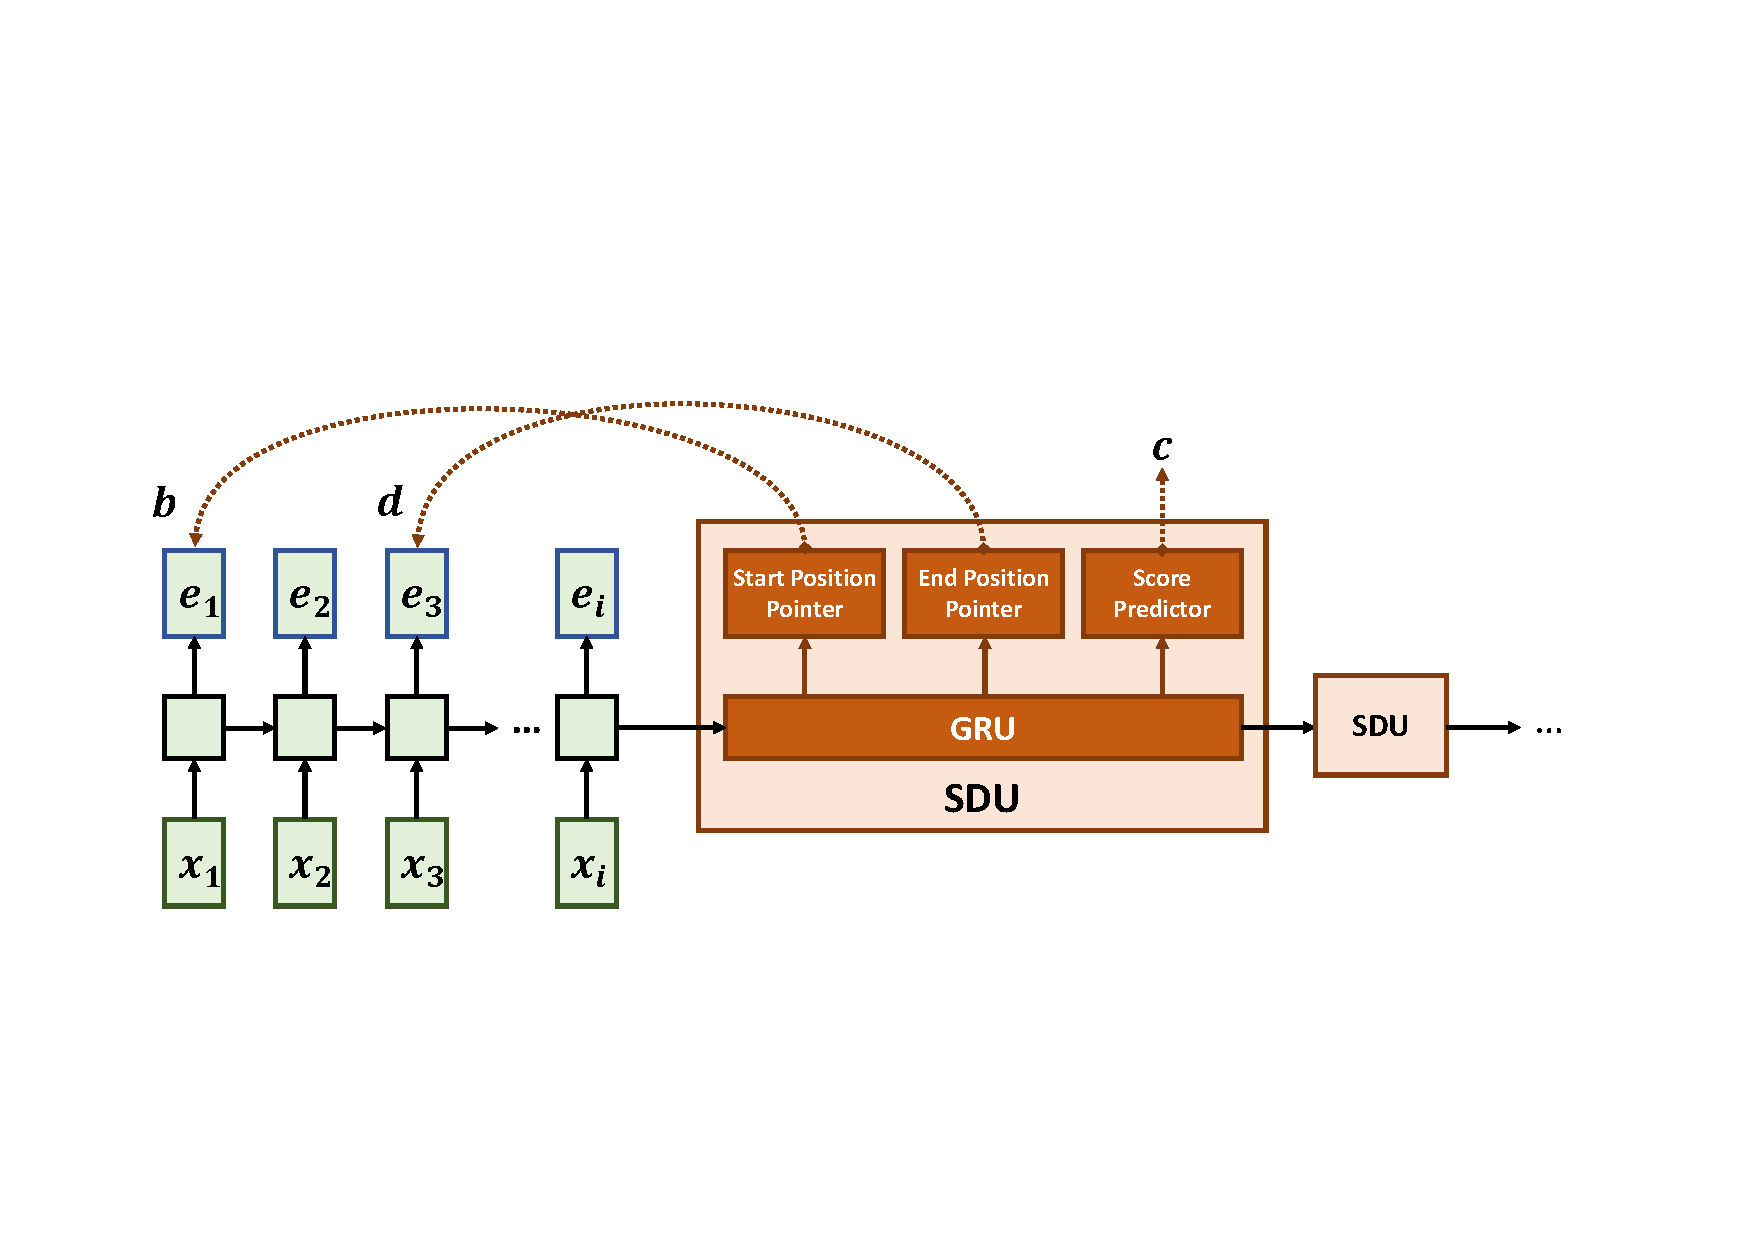
\includegraphics[width=\textwidth]{figures/figures/Figures2.pdf}
%    	\caption{Model overview\label{fig:model-overview}}
   \end{subfigure}
%    \begin{subfigure}[b]{0.45\textwidth}
%    	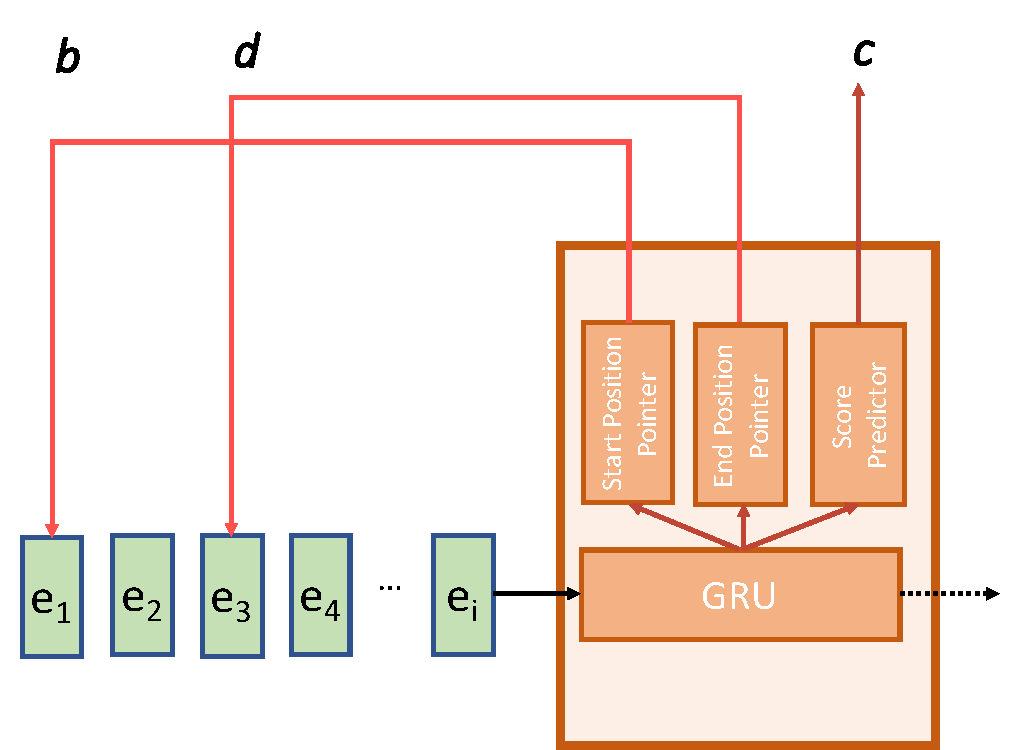
\includegraphics[width=\textwidth]{figures/figures/overview-module.pdf}
% 	\caption{Segment Detection Unit \label{fig:model-sbu}}   
%    \end{subfigure}  
   \caption{An Encoder (green) processes the input sequence to create a set of encoding vectors ($\{e_1, e_2,... e_M\}$). At each decoding step, a Segment Detection Unit (SDU) updates the decoding state with a GRU, and based on the updated state, the SDU points to the beginning ($\mathbf{b}$) and ending positions ($\mathbf{d}$) with two separate pointing modules and estimates the confidence score ($\mathbf{c}$) of the segment. \label{fig:model}}   
\vspace{-.05in}
\end{figure*}

\subsection{Model Overview}
The proposed \S2N is illustrated in Figure~\ref{fig:model}.  \S2N is a sequential encoder-decoder with an attentional mechanism~\cite{bahdanau2014neural}. \S2N sequentially encodes an input sequence $\x_1,\cdots,\x_M$ and obtains a corresponding sequence of encoding state vectors $\e_1,\cdots, \e_M$; the encoding state vector $\e_m$ essentially contains integrated information from $\x_1$ to $\x_m$~\cite{sutskever2014sequence,karpathy2015visualizing}. In the decoding stage at each step the Segment Detection Unit~(Section~\ref{sec:SDU}) outputs a temporal segment of interest $S_n$.

%During decoding, at each step the SDU receives the previous state and predict the three-element-tuple representing a segment.

% in contrast to the vanilla LSTM decoders or the attention-based decoders~\cite{luong2015effective}, we proposed to use Subsequence Boundary Unit (SBU), which we describe in the next section, to output a tuple $o_j = \{b_j, d_j, c_j\}$ that represents a subsequence. 

\subsection{Segment Detection Unit (SDU)\label{sec:SDU}}
A key component of the \S2N is the Segment Detection Unit~(SDU) for localizing a segment of interest in the decoding stage. As shown in Figure~\ref{fig:model}, the SDU is composed of four components: a Gated Recurrent Unit (GRU)~\cite{cho2014learning} for updating and communicating states between decoding steps, two pointing modules~\cite{vinyals2015pointer} for pointing to the beginning and ending positions of the segment, and a score estimator for evaluating the interest score of the segment. Details about these components are described below. 

\myheading{GRU for state update.} During decoding, at each step given the previous hidden state $\h_{j-1}$ ($\h_0$ is the concatenation of the last hidden state and memory cell of the encoder), the GRU module updates the current hidden state:
%\begin{align}
%% \z_j &= \sigma(\W_z [\h_{j-1}; \s_j ]) \\
%% \r_j &= \sigma(\W_r [\h_{j-1}; \s_j] ) \\
%% \hat{\h}_j &= \mbox{tanh}(\W [\r_j \odot \h_{j-1}; \s_j])\\
%% \h_j &= (1 - \z_j)\odot\h_{j-1} + \z_j \odot \hat{\h}_j
%\mathbf{h_{j}} = \mbox{GRU}(\mathbf{h}_{j-1}, \mathbf{z})
%\end{align}
$\mathbf{h_{j}} = \mbox{GRU}(\mathbf{h}_{j-1}, \mathbf{z})$, where $\mathbf{z}$ is a learned input vector to the GRU common to all the decoding steps. For further details about GRU, please refer to~Cho \etal \cite{cho2014learning}. 

S2N is a general framework and theoretically any RNN architecture, including LSTM and Depth-Gated Recurrent Neural Networks~\cite{yao2015depth}, can be used in place of the GRU. We propose to use GRU~\cite{cho2014learning} here because it has a simpler architecture and fewer parameters than the others (which means higher training and testing efficiency). We also experimented with LSTM but did not observe significant difference in terms of model accuracy. This is consistent with prior observations~\cite{buch2017sst} and empirical findings from prior work on deep recurrent models in other domains~\cite{cho2014learning,jozefowicz2015empirical,chung2014empirical}.

\myheading{Pointing modules for boundary localization.} Given the current state $\h_j$ of an SDU, we  predict the two boundary positions similar to the pointer networks (Ptr-Net)~\cite{vinyals2015pointer}. To localize the beginning position $b_j$ of a segment at decoding stage $n$, we use the pointer mechanism as follows:
\begin{align}
%u^{i}_{j} & = v^{T} \mbox{tanh}(\W_1 \e_i +  \W_2 \h_j), \\ % i \in (1, ..., M)\\
&b_n =  \myargmax{i} g(\h_n, \e_i),\label{eqn:eq1} \\
&g(\h_n, \e_i)  = \mathbf{v}^T \mbox{tanh}(\W_1 \e_i +  \W_2 \h_n ). \label{eqn:eq2}
\end{align}
The beginning boundary is determined as the location $i$ of the encoding sequence that has the highest correlation with the current decoding state ($\h_n$). To measure the correlation, we use a non-linear pointing function $g$. The output of this function depends on the state $\h_n$ of the SDU and the encoding vector $\e_i$ of the encoder component.

One alternative of predicting the locations is to use regression (similar to~\cite{liu2016ssd,redmon2016you}), however, this approach outputs a ratio in $[0, 1]$, which does not respect the constraint that the outputs map back exactly to the boundaries. As demonstrated in prior works~\cite{srivastava2015unsupervised,vinyals2015pointer}, the predictions are blurry and hence difficult to localize over longer sequences.   

Note the difference compared to the original Ptr-Net~\cite{vinyals2015pointer}: the pointer function is defined based on the encoding state vector $\e_i$ instead of the input vector $\x_i$. The encoding state vector $\e_i$ contains richer information than the input vector $\x_i$; $\e_i$ integrates the progression of the input time series up until time $i$, and this information is crucial for determining the segment boundaries~\cite{ma2016learning}. In the above, $\bf{v}$, $\W_1$ and $\W_2$ are learnable parameters of the pointing module that associates the decoding state with the hidden encoding states. 

Similarly, the ending position $d_n$ is determined using another independent Ptr-Net module. Thus, we have two Ptr-Net modules for determining the locations of the beginning and ending positions.

%where $\v$, $\W_1$ and $\W_2$ are learnable parameters of the attention model~\cite{bahdanau2014neural}. Note the difference compared to the original Ptr-Net~\cite{vinyals2015pointer}: we localize the pointer location by computing the maximum response of a function defined on the encoding state vector $\e_i$ instead of the input vector $\x_i$.  Compared to the input vector $\x_i$,  the encoding state vector integrates the progression of the input sequence up until time $i$, which is important for determining the segment boundaries~\cite{ma2016learning}.



% except that we use $\mathbf{\hat{h}}_j = \sigma (\mathbf{h}_j || \mathbf{e}_{d_j})$ in the place of $\mathbf{h}_j$ for Eq.(2) to consider the dependencies between the boundaries. $\sigma$ is implemented as 1D convolution and $||$ represents feature concatenation.



%\myheading{Score predictor}. Finally, we estimate the confidence score of the segment using a two layer 1D convolution network with a ReLu activation layer in between. \added[id=ZJ]{We will further explain what the score predictor captures in Sec.~\ref{}}
% \red{\bf Why call it as MLP when it is a convolution net? I don't understand the convolution operator here.} 
%\begin{align}
%  c_j = \mbox{Conv}(\h_j)
%\end{align}

% Note that essentially the order of predicting beginning and ending positions does not matter. We empirically observe that predicting the ending first leads to slightly better performance. We posit that the reason is that since the starting position is always in front of the end position (\emph{i.e.}, $b_j \leq d_j $), in a way $e_{d_j}$ can be seen as an informative prior. 
% The input $\mathbf{s}_j$ for the next step is computed as 
% \begin{align}
% \mathbf{s}_j = \mbox{Conv}(\mathbf{e}_{b_j} || \mathbf{e}_{d_j})
% \end{align}
\myheading{Score predictor}. Finally, we attach, $f_{score}$, a two-layer 1D convolution network on top of the GRU hidden state with a ReLu activation layer in between to predict $c_n$:
\begin{equation}
	c_{n} = f_{score}(\h_n)
\end{equation}
%how much the segment generated at a specific output order should be counted as useful output or not.
%We use the score $c_j$ as an indicator on how likely the output at decoding step $j$ should be considered an "valid" output. 

Note the $c_n$ is only based on the hidden state and not directly using information from $\x_i$ or $\e_i$, thus this score is not directly evaluating the quality of the segment, but rather and indicator of either accepting or discarding the output at $n$. It is possible to incorporate information from $\x_i$ or $\e_i$ into $f_{score}$, but this will significantly complicate the gradient flow during train. We will further explain what the score predictor captures in Sec.~\ref{sec:analysis}.

\myheading{No terminal output.} We do not design a terminal output for \S2N as in~\cite{bahdanau2014neural} because of two reasons. First, the problem we address is to output a ranked list of temporal segments of interest, which is different from the problem of sequence-to-sequence translation, in which there is a need for a terminal state. Second, by not having a terminal state, \S2N can output as many segments as needed, and later the output of score predictor could be used to select a subset of them, hence bringing flexibility to different needs in real-world problems. 



\section{\S2N Training} \label{sec:alignment}

The \S2Ns can be trained end-to-end. In this section, we first present the overall loss function (Sec.~\ref{sec:loss_function}), we then describe matching the sequence of predicted segments to the set of target segments using the Hungarian Matching with Lexicographic Cost (HMLC, Sec.~\ref{sec:HMLC}), we later analyze HMLC (Sec.~\ref{sec:analysis}) and compare it to its alternatives (Sec.~\ref{sec:alternatives_intro}) to demonstrate it effectiveness.

\subsection{Loss functions\label{sec:loss_function}}


%\subsection{Assigning predictions to ground truth~\label{sec:alignment}}
Training an \S2N requires a loss function that can measure the discrepancy between an unordered set of ground truth segments $\mG=\{G_1, \cdots, G_K\}$ and an ordered sequence of predicted segments $\mS=(S_1, \cdots, S_N)$. An strategy for matching $\mG$ to $\mS$ is to use an injective mapping: $f: \{1,\cdots, K\} \rightarrow \{1, \cdots, N\}$, where the ground truth instance $G_k$ should be matched to $S_{f(k)}$, and no two ground truth instances should be mapped to the same output segment (i.e., injection property: $f(k) \neq f(k')$ if $k \neq k'$).

Assume the assignment strategy is known for now, then the loss value for the predicted sequence of segments and the set of ground truth instances is computed as follows:  
\begin{equation}
	\mL(\mG, \mS, f) = \alpha \sum_{k=1}^{K}\mL_{loc}(G_k, S_{f(k)}) + \sum_{n=1}^{N} \mL_{conf}(S_n, \delta_n),
    \label{eq:loss}
\end{equation}
where $\delta_n$ is the $\{0, 1\}$ indicator for $S_n$ depending on whether $S_n$ is matched to a ground truth instance in $\mathcal{G}$. $\mL_{loc}$ and $\mL_{conf}$ are the loss functions for localization and label assignment,  which will be explained below.


Note that $\mL_{loc}$ only penalizes $K$ out of the $N$ $S_n$'s, the ones that are matched to the target segments in $\mG$. For the remaining $N-K$ unmatched segments, there is no localization penalty. 


% \begin{figure*}[t]
% \centering

%   \begin{subfigure}[b]{0.3\textwidth}
%   	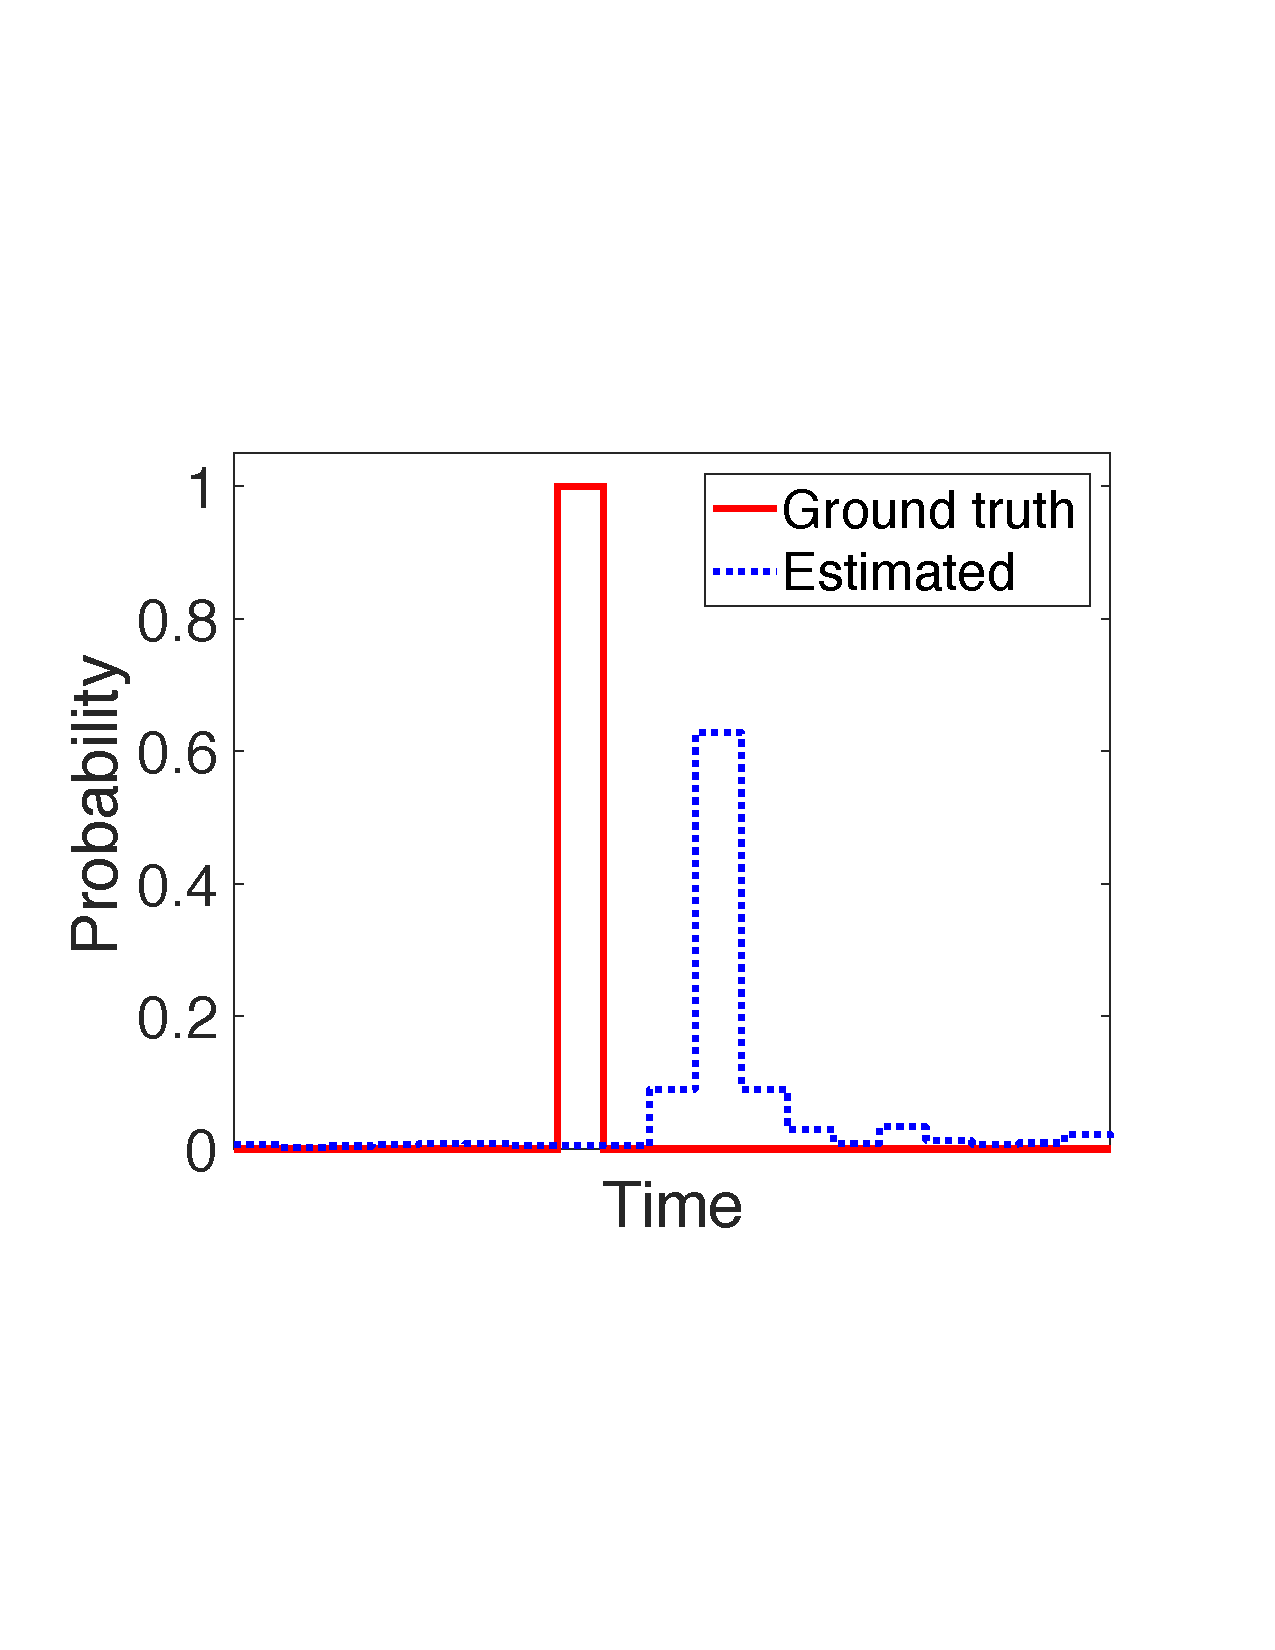
\includegraphics[width=\textwidth]{figures/score2_b.pdf}
%     \caption{Cross-entropy binary loss\label{fig:Cross-loss}}
%   \end{subfigure} 
%      \begin{subfigure}[b]{0.3\textwidth}
%   	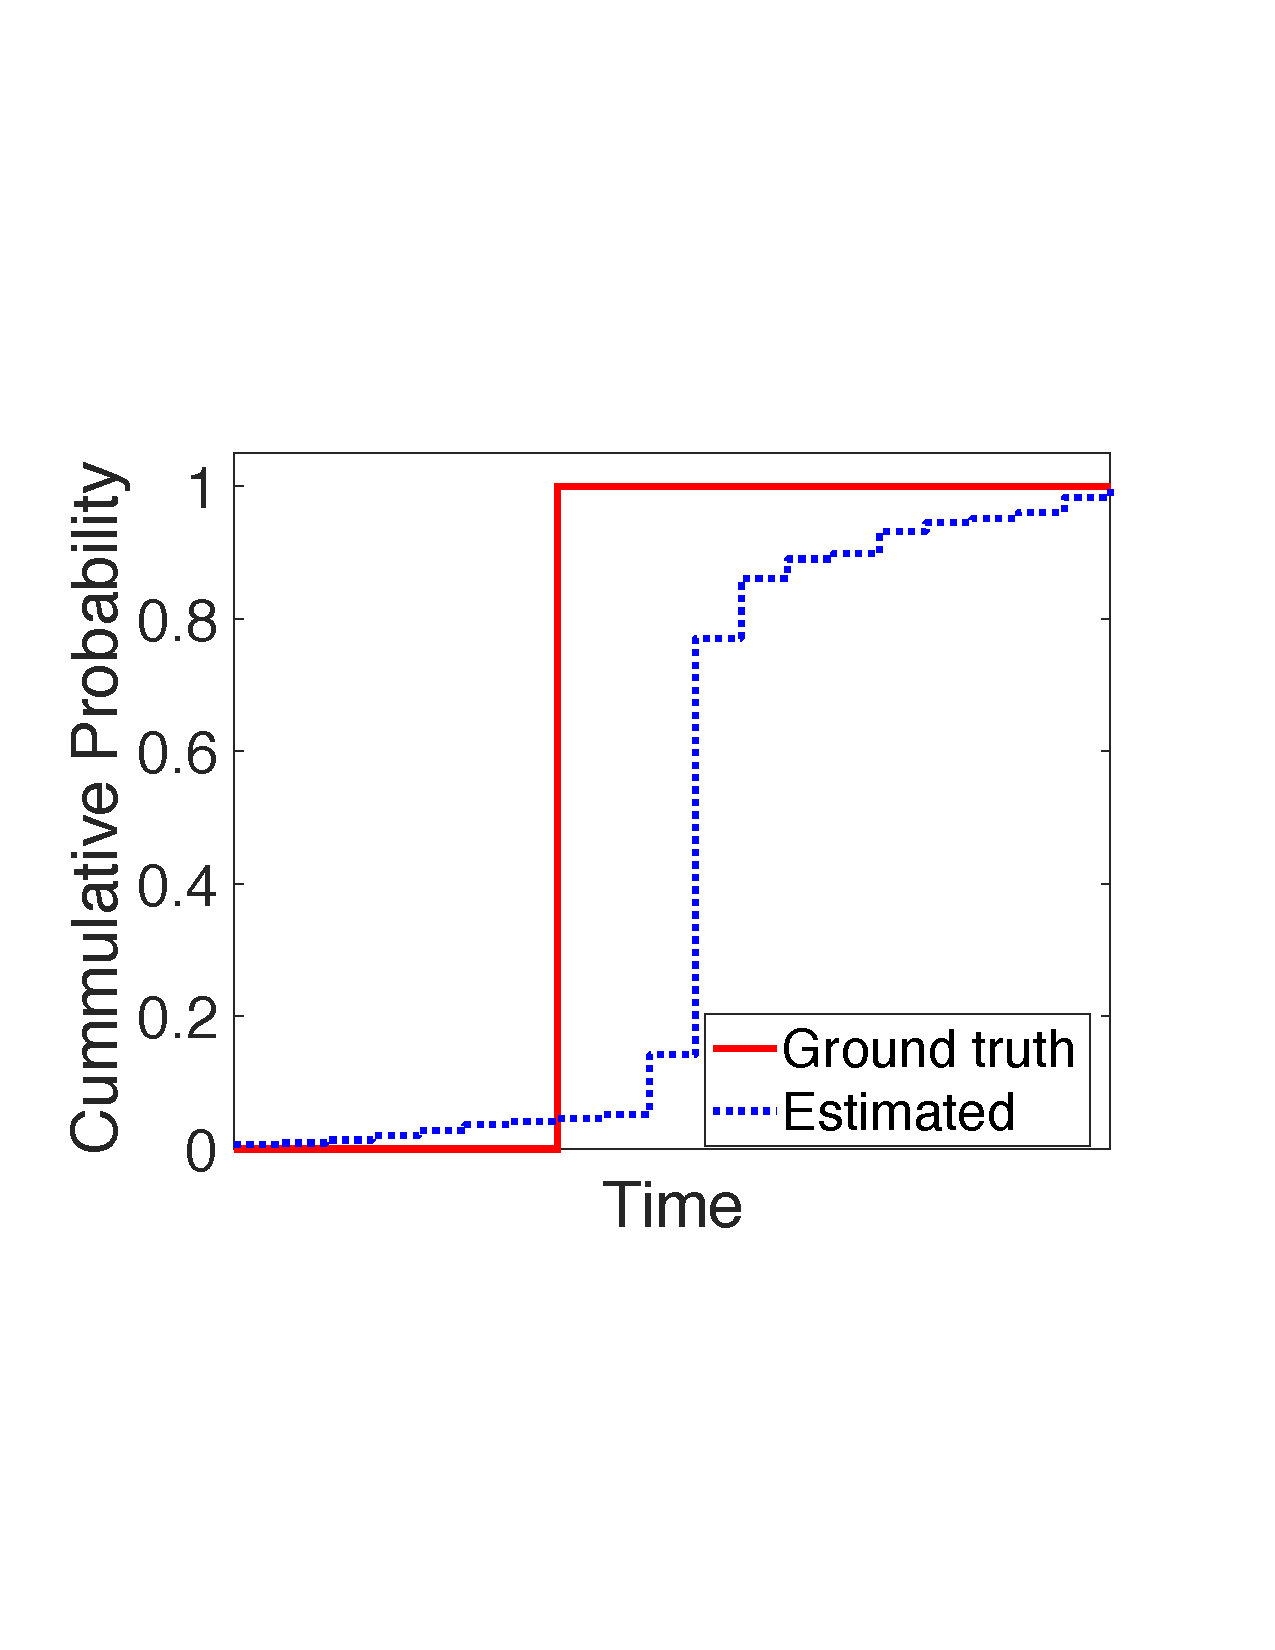
\includegraphics[width=\textwidth]{figures/score_cum2_b.pdf}
%         \caption{L2 loss \added[id=ZJ]{Needs modification}\label{fig:L2-loss}}
%   \end{subfigure}
%   \begin{subfigure}[b]{0.3\textwidth}
%   	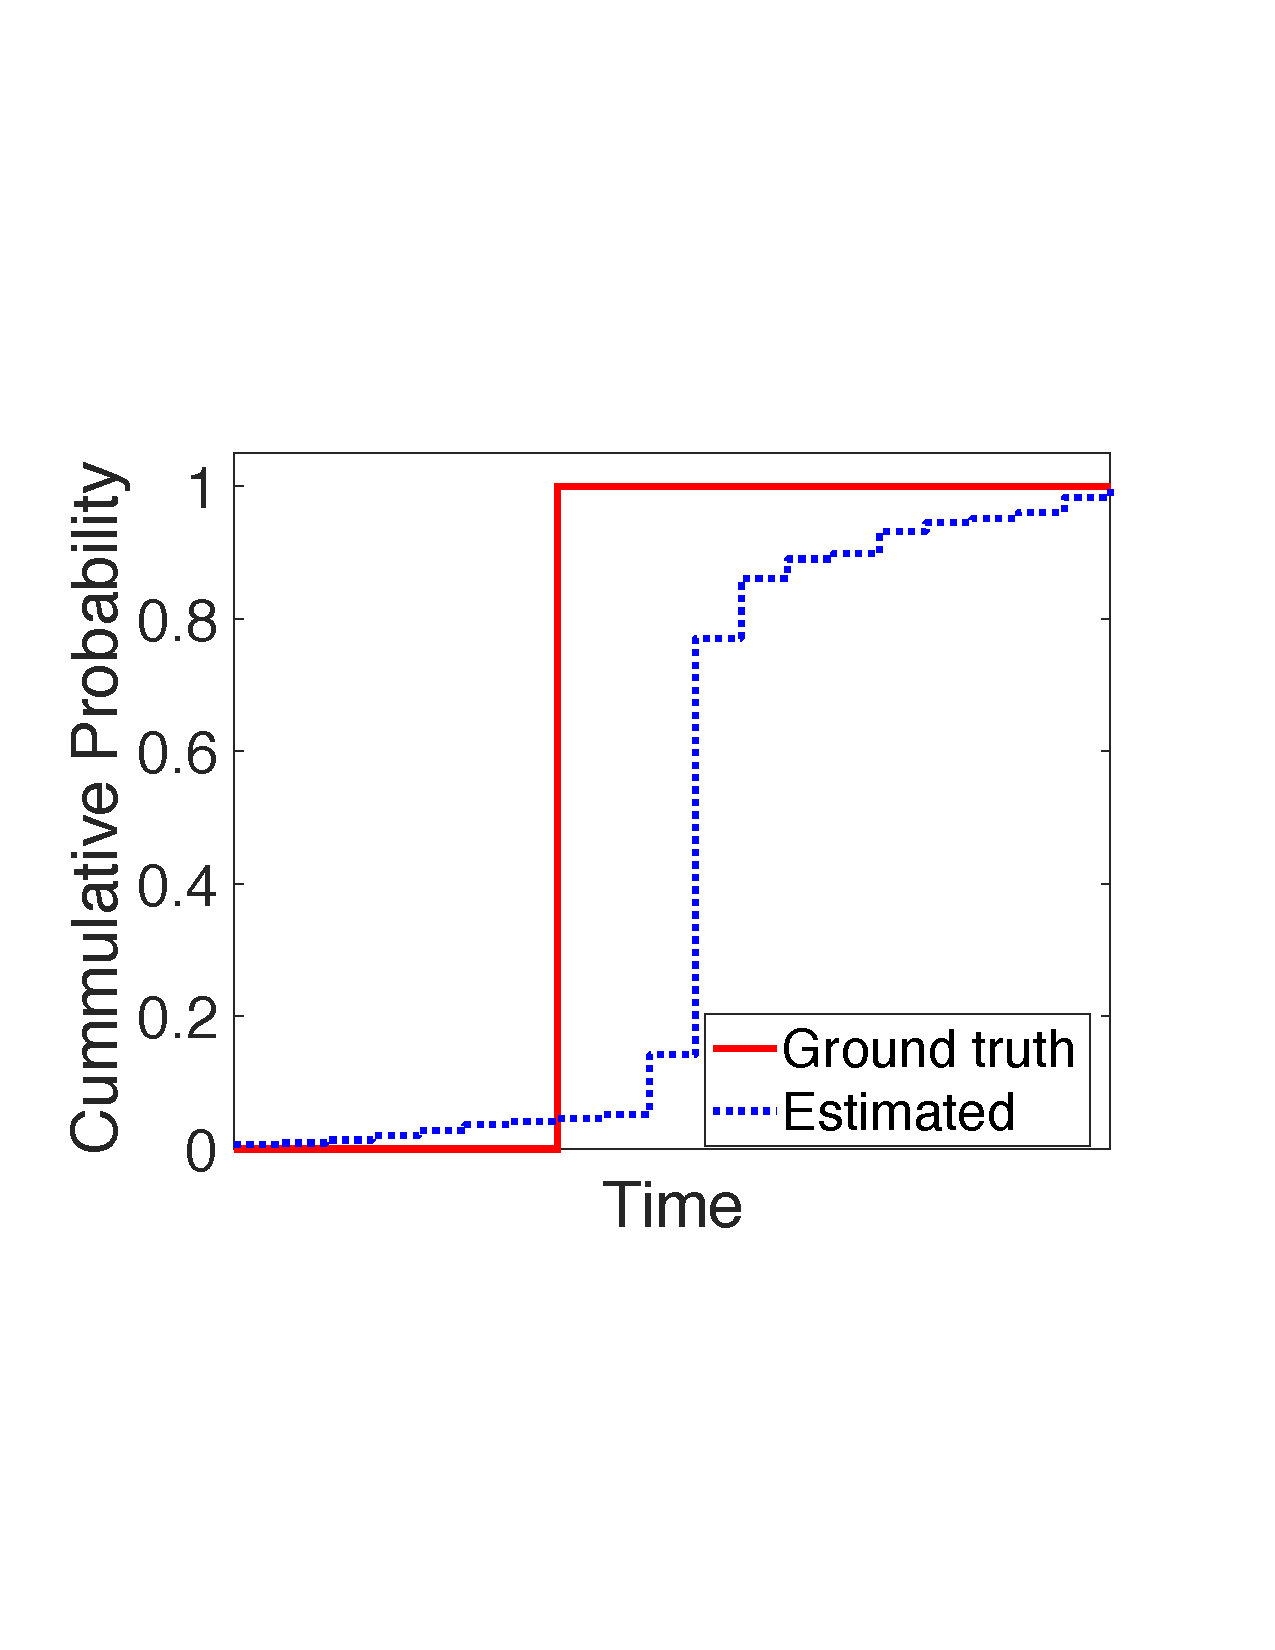
\includegraphics[width=\textwidth]{figures/score_cum2_b.pdf}
%         \caption{EMD loss~\label{fig:EMD-loss}}
%   \end{subfigure}   
% %    \vskip -0.1in
%   \caption{\added[id=ZJ]{TODO} Benefit of EMD distance\label{fig:cumsum}}
% \end{figure*}   

\myheading{Loss function for localization.} Let us now explain how the loss $\mL(G_k, S_{f(k)})$ is defined. Our goal is to use a loss function that can indicate the {\em level} of discrepancy between a predicted segment and a target segment. The surface of the loss function should vary smoothly without any flat regions; flat regions have zero gradients and it will be difficult for gradient-based optimization.

One way to define the localization loss is to frame the boundary localization as a multi-class classification problem and use the cross-entropy loss as in~\cite{vinyals2015pointer}.  Recall that the pointer function $g$ can be used to calculate the probability distribution over the location of the segment boundary: \emph{i.e.}, using $\{g(\h_n, \e_1), ..., g(\h_n, \e_M)\}$. However, this loss function is unsuitable for boundary localization because it is insensitive to the amount of localization error; this loss function has zero gradients when the target boundary is not close to the predicted boundary. Another alternative is to use the Mean Squared Error (L2) loss, but this loss function is also unsuitable for the same reason. 
%because the desired localization is not a real-valued function of each hidden state with a certain amount of irreducible Gaussian noise, with constant mean and variance. 

% as shown in Figure~\ref{fig:Cross-loss}. \added[id=ZJ]{L2 loss is also not enough since XXX}.

 We propose to use a loss function that is defined based on the Earth Mover's Distance (EMD) between the probability distribution of the predicted boundary and the distribution that represents the ground truth boundary. We now explain how this loss function can be computed for the beginning position $b$ (the loss for the ending position $d$ is computed similarly).  Recall from Eq.~(\ref{eqn:eq2}) that  we determine the beginning location of a segment as the maximum of a response function: $b =  \myargmax{i} g(\h_{f(k)}, \e_i)$, where $\h_{f(k)}$ is the state vector of the SDU. We define the probability of picking $i$ as the boundary point based on the soft-max function 
\begin{align}
Pr(b =i) = \frac{\exp(g(\h_{f(k)}, \e_i))}{\sum_{i=1}^{M} \exp(g(\h_{f(k)}, \e_i))}.	
\end{align}
Let $\p^*$ be the binary indicator vector for the ground truth location of segment boundary; $p^*_i =1$ if $i$ is the annotated boundary and $0$ otherwise. The EMD loss can be computed based on the differences the two cumulative distributions: 
\begin{align}
\mL_{loc}^b(G_k, S_{f(k)}) = \sum_{m=1}^{M} \left( \sum_{i=1}^m Pr(b=i) - \sum_{i=1}^m p^*_i\right)^2.\label{eq:emd}
\end{align}

% For the localization loss, different than the pointer loss that simply points to a position and optimize based on a single label classification loss. In this paper, we adopt Earth Mover’s Distance~\cite{rubner2000earth} (EMD, also known as Wasserstein distance) to penalize based on the distance between the predicted positions and the ground truth positions. Take for example predicting the ending position of a segment: $\{p(d = i | h) | i=1, ... N\}$ be the predicted probability of the ending index, let $\mathbf{t}$ be a one hot vector indicating the ground truth location. The EMD distance between $p$ and $t$ is 
% \begin{equation}
% 	E_{E}(p, t) = \sum_{i=1}^{N}(CDF_{i}(\mathbf{p}) - CDF_{i}(\mathbf{t}))^2
% \end{equation}
Here, we use sum of squared differences in Eq.~(\ref{eq:emd}) instead of sum of absolute differences because the former is easier to optimize with gradient descent~\cite{hou2016squared,shalev2011stochastic,luenberger1973introduction}.  The loss for the predicting the ending position is similarly defined and the total localization loss is:  
\begin{align}
\mL_{loc}(G_k, S_{f(k)}) = \mL_{loc}^b(G_k, S_{f(k)})+ \mL_{loc}^d(G_k, S_{f(k)}). 	
\end{align}

We will provide empirical comparison between the proposed EMD loss and the $L_2$ loss and the  cross-entropy loss in Section~\ref{sec:video-highlight}.

\myheading{Loss function for confidence estimation.} The \S2N will produce a sequence of segments; some will be matched to a ground truth segment and some will not be. Ideally, we want the former type to have high confidence value while the latter to have low confidence value. The loss function for confidence estimation is designed to satisfy this desired criterion. 
Recall that the \S2N predicts a confidence value $c_n$ at each decoding step $n$, and $\delta_n$ indicates whether there is a matching target segment for this decoding step. We use the cross-entropy loss to measure the compatibility between $c_n$ and $\delta_n$: 
\begin{align}
\mL_{conf}(S_n, \delta_n) = - \delta_n\log(c_n) -  (1- \delta_n)\log(1 - c_n).
\end{align}
As we will show in Sec~\ref{sec:analysis}, $c_n$ is an indicator on how likely we should accept the predict segment at $n$.
 

%For some applications, such as video summarization, the desired confidence value for each segment $S_n$ is not necessary binary. In this case, we can use the $L_2$ loss function, i.e., $\mL_{conf}(S_n, \delta_n) = (c_n - \delta_n)^2$. 

\subsection{Assignment Strategy: Hungarian Matching with Lexicographic Cost (HMLC)~\label{sec:HMLC}} 

As shown in Eq.~(\ref{eq:loss}), an important component of the loss computation process is to match the target segments $\mG$ to the predicted ones $\mS$. Inspired by~\cite{stewart2016end}, we propose to use a bipartite matching strategy called the Hungarian Matching with Lexicographic Cost (HMLC). Specifically, we define the matching cost between a predicted segment $S_n$ and a ground truth $G_k$ using a triplet cost function:
\begin{equation}
\Delta (G_k, S_n) = (o_{kn}, -n, l_{kn}).\label{eq:assign}
\end{equation}

The function $\Delta: \mathcal{G} \times \mathcal{S} \rightarrow \Re^3$ returns a tuple where $l_{kn}$ is the $L_1$ distance between $G_k$ and $S_n$ (or IoU distance). $-n$ is an integer indicating the negation of the output order of $S_n$ (the earlier the output, the higher the reward).
$o_{kn}$ indicates whether there is significant overlapping between $G_k$ and $S_n$: 

% $o_{kn} = 0$ if $IoU(G_k, S_n) \geq 0.5$ and $1$ otherwise ($IoU$ denotes the intersection over union function). 

%

\begin{figure*}[t]
\centering

  \begin{subfigure}[b]{0.18\textwidth}
   	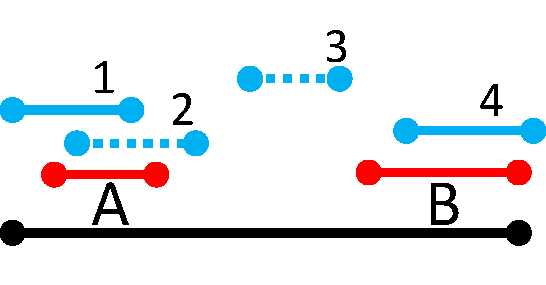
\includegraphics[width=0.9\textwidth]{figures/Matching/HMLC_example.pdf}
    \caption{\label{fig:HMLC_example}}
   \end{subfigure} 
     \begin{subfigure}[b]{0.18\textwidth}
   	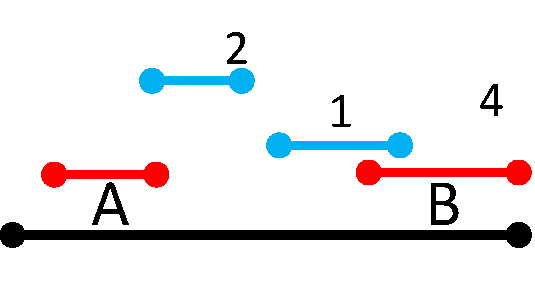
\includegraphics[width=0.9\textwidth]{figures/Matching/Tied.pdf}
        \caption{\label{fig:tied}}
   \end{subfigure}
  \begin{subfigure}[b]{0.18\textwidth}
   	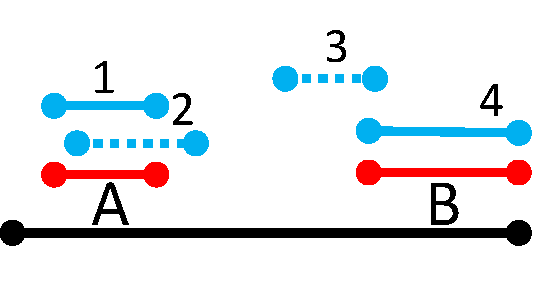
\includegraphics[width=0.9\textwidth]{figures/Matching/HMLC_r1.pdf}
        \caption{\label{fig:HMLC_r1}}
   \end{subfigure}   
     \begin{subfigure}[b]{0.18\textwidth}
   	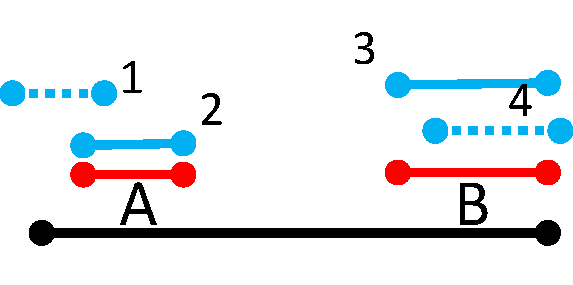
\includegraphics[width=0.9\textwidth]{figures/Matching/HMLC_r2.pdf}
        \caption{\label{fig:HMLC_r2}}
   \end{subfigure}  
        \begin{subfigure}[b]{0.18\textwidth}
   	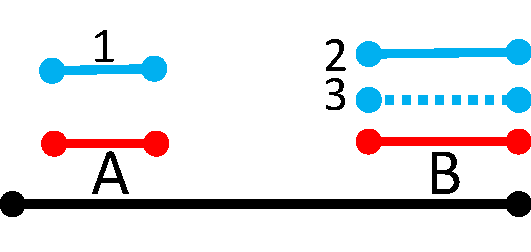
\includegraphics[width=0.9\textwidth]{figures/Matching/HMLC_r3.pdf}
        \caption{\label{fig:HMLC_r3}}
   \end{subfigure}  
%    \vskip -0.1in
   \caption{Illustration of the HMLC assignment strategy. HMLC encourages \S2N to generate highly overlapped segments with ground truth and generate true positive segments earlier than false positive ones. Given an input frame sequence (black line), the segments in red (A, B) represent the target segments (ground truth) and the segments in blue (1, 2, ...) are the sequentially generated segments. The solid lines are assigned with ground truth and the dashed lines are false positives.
   , the numbers also represent the output order. \label{fig:HMLC-illurstration}}
\end{figure*}   

\begin{figure*}[t]
\centering

  \begin{subfigure}[b]{0.20\textwidth}
   	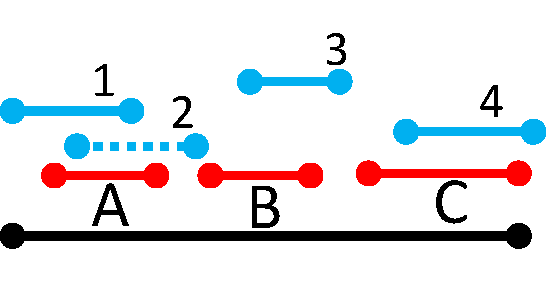
\includegraphics[width=\textwidth]{figures/Matching/HMLC.pdf}
    \caption{HMLC\label{fig:HMLCM}}
   \end{subfigure} \hspace{6ex}
     \begin{subfigure}[b]{0.20\textwidth}
   	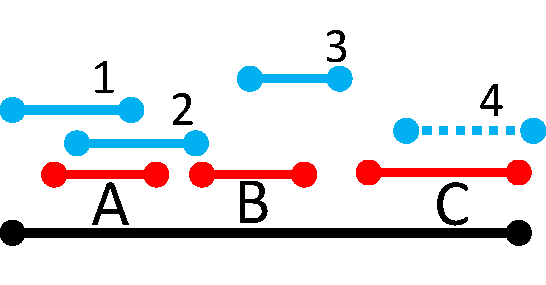
\includegraphics[width=\textwidth]{figures/Matching/Fix.pdf}
        \caption{Fix\label{fig:FixM}}
   \end{subfigure}\hspace{6ex}
  \begin{subfigure}[b]{0.20\textwidth}
   	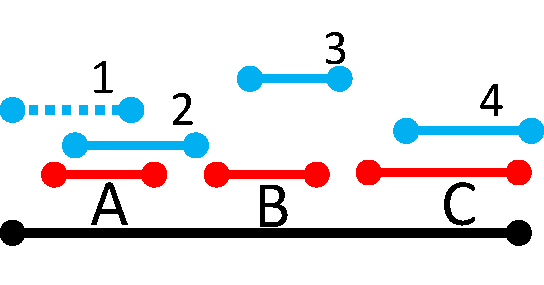
\includegraphics[width=\textwidth]{figures/Matching/Greedy.pdf}
        \caption{Greedy\label{fig:GreedyM}}
   \end{subfigure}   \hspace{6ex}
     \begin{subfigure}[b]{0.20\textwidth}
   	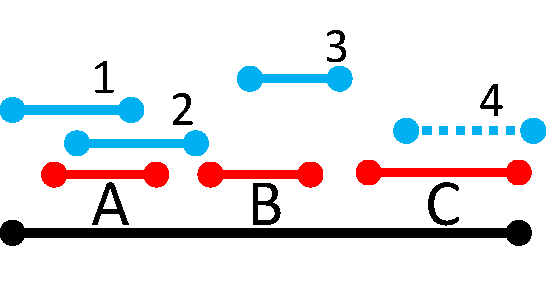
\includegraphics[width=\textwidth]{figures/Matching/TopK3.pdf}
        \caption{TopK (3)\label{fig:TopK3M}}
   \end{subfigure}  
%    \vskip -0.1in
   \caption{Illustration of alternative assignment strategies. Given an input frame sequence (black line), assume there are three ground truth segments (A, B, C in red) and the \S2N sequentially generates four segments 1, 2, 3, and 4.  Different assignment strategies will assign the predicted segments to the ground truth segments differently; solid blue lines indicate matched predictions, dashed blue lines indicate unmatched predictions. (a) HMLC matching (1-A, 3-B, 4-C); (b) Fixed order matching (1-A, 2-B, 3-C); (3) Greedy matching (2-A, 3-B, 4-C);  (4) TopK matching  for $K=3$ (2-A, 3-B, 1-C)\label{fig:different-matching}}
\end{figure*}   

\begin{equation}
 o_{kn}=\begin{cases}
              1 \hspace{3ex} \mbox{if $IoU(G_k, S_n) \geq 0.5$} \\
              0 \hspace{3ex} \mbox{otherwise}. \label{eq:oij}
           \end{cases}
\end{equation}
We can use the Hungarian algorithm to determine the best matching with lexicographic preference: 
\begin{align}
	f^{*} & = \myargmax{f} \sum_{k=1}^K \Delta(G_k, S_{f(k)}) \nonumber \\
	      & = \myargmax{f}\left(\sum_{k=1}^{K} o_{kf(k)}, \sum_{k=1}^{K} -f(k), \sum_{k=1}^{K} l_{kf(k)} \right).
\end{align}
The Hungarian algorithm first maximizes the total number of matches (i.e., using $o$). For tie-breaking, it will consider the order of segments (i.e., $n$), and finally the amount of overlapping (i.e., $l$) if necessary. Analysis of HMLC in the case of matching the predicted temporal segments to the targets will be presented next.
%For more details, see~\cite{stewart2016end}.

\subsection{Analysis\label{sec:analysis} of Assignment Strategies}
Designing an appropriate assignment strategy is crucial for guiding \S2N to generate meaningful results in expected order. For many applications, we want the \S2N to: (1) generate segments that have high overlap with the ground truth, and (2) generate true positive segments earlier than false positive ones. In this section, through some examples, we will illustrate how the proposed assignment strategy will satisfy these desired criteria. 

Let us start with a situation shown in Figure~(\ref{fig:HMLC_example}), in which the black line at the bottom is an input sequence, the red lines $A$ and $B$ are two ground truth segments. Assume for now \S2N outputs sequentially four segments: 1, 2, 3 and 4, in that order. In this example, assume Table~\ref{tab:HMLC} represents the pairwise matching scores between the predicted segments 1, 2, 3, 4 to target segments A and B. Based on the scores, matching 1 to A and 4 to B gives the highest reward. 

%\added[id=ZJ]{TODO: add the Tab for scores.}


\setlength{\tabcolsep}{8pt}
\begin{table}
 \centering
 \begin{tabular}{c  c  c  c c}
 \toprule
& \multicolumn{4}{c}{Predicted segments} \\
\cmidrule{2-5}
   &  1 &  2 & 3 & 4   \\
\midrule 
 A &  (1, -1, 0.7) & (1, -2, 0.8) & (0, -3, 0.0) & (0, -4, 0.0)  \\
% \hline
 B &  (0, -1, 0.0) & (0, -2, 0.0) & (0, -3, 0.0) & (1, -4, 0.8) \\ 
 \bottomrule
 \end{tabular}
 \caption{Lexicographic Cost between generated segments and ground truth in Figure~\ref{fig:HMLC_example}\label{tab:HMLC}}
 \end{table}


In general, the first two components ($o_{kn}$ and $n$) of the lexicographic cost triplet (Eq.~\ref{eq:assign}) are sufficient for most of the matching problems. However, in the early training stage, it is possible that none of the predicted segments has significant overlap with a ground truth, as shown in Figure~\ref{fig:tied}. In this case, the third component of the triplet cost function is used to encourage small and stable adjusting of the predicted segments toward the targets. 

Note that the HMLC itself does not guarantee a loss function that explicitly optimizes for the expected output. Theoretically it is possible to have the trained \S2N output results like the ones in Figure~\ref{fig:HMLC_r1} or Figure~\ref{fig:HMLC_r2}, which is not optimal if we consider the ordering of the output segments. By designing the matching algorithm to prefer early predictions, these situations were rare. This is mostly because that in the initial training stages the cost induced by the order of the segments plays an important role in determining the matching. During the training stage, assume that each predicted segment has the same probabilities to overlap with a ground truth, with the introduction of a reward for preferring early detections, most of the time the early predictions will be matched with ground truth.


Similarity, for the score predictor, since the early outputs are likely to be matched with ground truth, the expected score of the early predictors are more likely to be 1. In this way, it becomes an indicator of the number of ground truth in an input sequence.
  

% Another potential issue of 

%
%
% 
%
%
%
%
%
%
%\textbf{Effect on proposals}: creates multiple outputs that tend to pointing to similar outputs. However, for each output serious, the diversity is enforced.
%
%\textbf{Effect on score predictors}: a weak indicator of the possible number of outputs.
%
%\textbf{Relationship to Optimizing Average Precision}: As shown we want to be early/high overlap.But it doesn't directly optimize the lexcion loss. Since it order is not directly derivative. but it implicitly learns it. We will leave it as future work.

\subsection{Alternative Assignment Strategies~\label{sec:alternatives_intro}}
HMLC is rather sophisticated but it was found to be very important in our experiments. There are simpler alternatives, but they have some limitations compared to HMLC. 
%We will discuss some alternative strategies and their limitations in this subsection. 

% satisfy what we require. 

%In this section we further show the advantage of using HMLC by comparing it to several straight-forward alternatives.


 \myheading{Fixed Order Matching.} Perhaps the most straight matching strategy is to machine the output of \S2N sequentially to the target segments following some natural order, \emph{e.g.}, from left to right. We denote this matching \emph{FIX}. For example, for all the cases shown in Fig.~\ref{fig:HMLC-illurstration}, fixed matching simply assigns 1 to A and 2 to B regardless of their positions relatives to the target segments.  The limitation of the fixed order matching is that it might incorrectly assign candidate hypotheses to ground-truth segments when the decoding process produces false positives as shown in Figure~\ref{fig:FixM}. Additionally, it will enforce a strong location bias that limits its generalization abilities. For a exactly video with 2 segments. The order of A and B should not make a difference.
 
% \added[id=MH]{Need to explain what fixed order matching is. This section also contains incorrect reference. Check.} 
 

 
% \added[id=MH]{Need to explain Top K and greedy matching.}
 
\myheading{Top K Matching} Top K matching (denoted as \emph{TopK}) is a simplified version of HMLC by zeroing out the first item in the triplet cost. \emph{i.e.},  only the first K outputs were considered in the matching strategy, then it decides  which target to match to based the L1 distance.  However, deciding the number of K is not trivial, additionally, as shown in Figure~\ref{fig:TopK3M}, it may cause significant change of the localization losses (by matching  1-C), which causes instabilities in training.

\myheading{Greedy Matching}: Another strategy for matching is to simply match the generated segments to the closest targets solely based on their distance. We denote this strategy as $Greedy$. This is by zeroing out the first and second item in the triplet cost of HMLC. Despite that it shares the same shortcomings as the TopK matching, it also does not enforce an order.


We will show more emperical results in Sec~\ref{sec:improved-S2N-exp}.  


%The proposed cost function prioritizes the recall value, but it also sets the preference for using the earlier output segment in case of repeated detections. For example, when two output segments significantly overlap with the same ground-truth (\emph{e.g.}, Segments 1 and 2 in Figure~\ref{fig:match}), it will match the ground truth instance $A$ to Segment 1 since Segment 1 is produced earlier than Segment 2.

% (\red{\bf Check if the second term of the loss can be simplified further using the inverse function of $f$ or $f$ itself. Also check if the loss is correct. Do you want to low the score of the non-match segments instead of the matched segments.})

% We need to cross-valid for the best $\alpha$

% The crux then become how to find the most appropriate matching between $G$ and $C$.  A naive approach would be a simple fixed ordering matching strategy. We sort the ground truth by position from left to right. This fixed order matching sequentially assigns candidates to the sorted ground truth. However, a limitation of this is that it might incorrectly assign hypotheses to ground truth instances when the decoding process produces false positives or false negatives. 

% A better injection $f: G \rightarrow C$ is based on the hungarian loss proposed in~\cite{stewart2016end}. Recall that one of the principled objectives of our model is to output a coherent sequence of predictions on multiple objects. We define the stopping criterion for the generation process to be when a prediction score falls below a specified threshold. 




% Note that the matching not be included in the gradient desent computation graph.

%\subsection{Loss functions}
%As shown in Eq.~\ref{eq:loss}, the loss function for training an \S2N is composed of two terms: the localization loss and the score confidence loss.

%One approach to define the localization loss is to 



% However, for applications such as video action proposal, the ground truth are scarce to ensure high recall rate. Augmenting the ground truth with random subsequences that are partially overlap with ground truth is a general way to address this issue. However, treating them indiscriminately as ground truth will degrade the performance of \S2N. To combat this issue, we associate the prediction score with their overlap with the ground truth:
% \begin{align}
% l_{score} (c_m) =\begin{cases}
%                (\frac{c_m}{\mbox{overlap}} - 1)^2, \mbox{if positive} \\
%                (c_m)^2, \mbox{otherwise} \label{eq:l-score}
%             \end{cases}
% \end{align}



%\subsection{Auxiliary Loss}
%\begin{wrapfigure}{R}{0.3\textwidth}
%\centering
%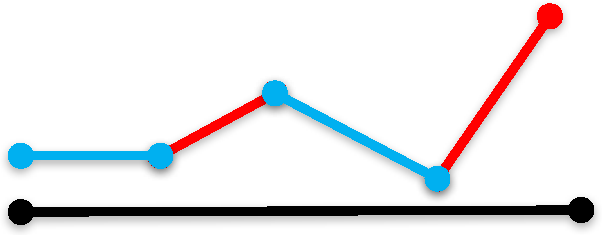
\includegraphics[width=0.25\textwidth]{figures/figures/mono.pdf}
%\caption{\label{fig:mono}Expected progression of the \textbf{Cumulative Averaged Actionness} scores on video temporal space (black) with actions (Red) and non-actions(Blue).}
%\end{wrapfigure}
%As shown in Figure~\ref{fig:mono}, we want the encoded temporal features to have some properties mentioned in week 13 slides. We can pre-train it to enforce the ranking comparison. We can make the enforcement in the encoding stage as follows:
%
%For a sequence of frames $x_1, x_2, x_3, ..., x_s, ..., x_e,... x_N$ where $x_s$ and $x_e$ are the start and end of an action respectively. Our LSTM encodes $e_1, e_2, ... e_N$ at each encoding step. We need to enforce that $e_1 > e_2>e_3>e_s<e_{s+1}<e_{s+2} ... < e_e > e_{e+1} > ...$. This is similar to the semantic constrains in~\cite{buch2017sst} and video darwin~\cite{fernando2015modeling}.
%
%The same idea is described in~\cite{ma2016learning}. We need the encoder to model the progresssion patterns of the activities in training. Since we only care about on class. The ranking can be simplified as:
%\begin{equation}
%\mathcal{L}_{r}^{t} = max(0, -\delta _t (p_t - p_{t-1}) +\alpha )
%\end{equation}
%Where $p_t$ is the "culmulative average actionness" score at time $t$. If $p_t$ is action, $\delta_t = 1$, otherwise $\delta_t = -1$.



% \subsection{Sequential encoder-decoder networks with attention}
% Our network falls in the category... but designed to predict segments. Based on the hidden sate in decoding, we predict XXX Our networks localizaiton module is based on Ptr-Net, which output locations depends on
% the number of elements in the input sequence.
% % \subsection{Pointer Networks}
% \subsection{Training Recurrent Models for Sequence Generation}
%  Suitable loss functions have previously been proposed in structured speech recognition and natural language processing~\cite{graves2006connectionist,stewart2016end}. Here we formulate such a loss function our problem

% \subsection{Video Summarization and Temporal Action Proposal Generation}
% I will do it!


\section{Experiments}
% In this section we first of demonstrate some nice properties of SPN on synthetic datasets. We then demonstrate the effectiveness of the SPN on two challenging problems - sentence chunking and video action proposal.

In this section we show that \S2N achieves state of the art performance on multiple different tasks: video summarization, video highlighting, and action proposal generation. Detailed analysis will be provided for all cases, with a slight emphasis on the task of action proposal generation because it is more complex than video highlighting and video summarization. 

\subsection{Model Implementation and Hyper-parameters}
We used the same architecture in all experiments even though better results can likely be achieved by tuning the model to fit specific problems. 
%there are likely some gains to be obtained by tuning the model to fit specific problems. 
%We felt that having the same model operate on all the problems would make the main message of the paper stronger. As a result, 
Unless specified otherwise, the encoder is a two layer bi-directional GRU with 512 hidden units with dropout rate 0.5, the GRU module in SDU is one-directional with 1024 hidden units. All the models are trained with the Adam optimizer~\cite{kingma2014adam} for 50 epochs with an initial learning rate of 0.0001, which was decreased by a factor of 10 when the training performance plateaued, batch size of 32 and $L_2$ gradient clipping of 1.0. The trade-off factor $\alpha$ in Eq.~(\ref{eq:loss}) is set to ensure that $\mL_{loc}$ does not dominate in the total loss. 
%\added[id=ZJ]{Throughout all the experiment we set $\alpha$ to be X}.
A weight adjustment for the score predictor is also used if necessary to account for the imbalance between the positive and negative samples. 

% The code is publicly available at \url{https://www3.cs.stonybrook.edu/~cvl/projects/wei2018s2n/S2N_NIPS2018s.html}

\subsection{Video Highlights Detection~\label{sec:video-highlight}}
Video highlights detection aims to detect one temporal clip which is the most salient event for each video. In this section, we show that \S2N can be trained to be a highlight detector by generating one segment per video.

\myheading{Dataset.} We adopted the large-scale VTW dataset~\cite{zeng2016generation} for video highlight detection. The VTW dataset contains 18100 videos, originally proposed for video captioning task. A subset of the dataset were labeled with temporal locations of highlight shots. We followed the same train/test split as in~\cite{zhang2018retrospective}: the first 1500 videos were for training, and the next 500 videos were for testing. The average duration is 1.5 minutes, about 2000 frames for each video.

\myheading{Implementation.}
For each video, we extracted I3D features~\cite{carreira2017quo} on RGB frames. We used linear interpolation to get fixed length sequence of features for each video (here we set as 150). Since each video only contain one highlight segment, we set the number of segments to be 1 for \S2N.

\myheading{Evaluation metric.} We followed the commonly used F1-scores to evaluate the similarity between predicted highlight segments and ground truth segments. 

\myheading{Baseline.} We compared \S2N with three state-of-the-art video highlight detection algorithms on the VTW dataset: DPP-LSTM~\cite{zhang2016video}, Hierarchical-RNN~\cite{zhao2017hierarchical}, and retrospective sequence-to-sequence model~\cite{zhang2018retrospective}. Both~\cite{zhao2017hierarchical} and~\cite{zhang2018retrospective} adopt a hierarchical model to extract features from videos: first the original video is divided into multiple segments, within each segment, an RNN-based encoder is used to extract features for the segment; then a higher level RNN is used to incorporate segment-wise features. However, these methods require additional parameters and increase the probability of overfitting. In our method, for simplicity, we ignore hierarchical structure and use the segment-wised feature extracted from pre-trained networks as input to our system. As we will show next, \S2N is quite robust to different features.

\myheading{Results.} Tab~\ref{tab:highlight} shows the F1 scores of the proposed \S2N and other methods. As can be seen, \S2N achieves the best performance. 


\myheading{Ablation Study.} To understand the importance of the EMD loss, we performed some controlled experiments by replacing the EMD loss in \S2N with other alternatives. We compare with the cross entropy loss and the $L_2$ loss discussed in~\ref{sec:loss_function}.  Clearly, the proposed EMD loss is able to guide the pointer network to point to the correct starting and end positions.

We have also experimented with the original pointing mechanism proposed in the~\cite{vinyals2015pointer}. Specifically, rather than using Eq.~\ref{eqn:eq1} that localizes the boundaries based on the correlation between hidden states and the decoding states, the implementation in~\cite{vinyals2015pointer} are based on the input features: $b_n =  \myargmax{i} g(\h_n, \x_i)$. We got significantly worse results following~\cite{vinyals2015pointer}. This suggests that compared to the input feature $\x_i$, the hidden state $\h_i$ captures more progressive information, which is crucial for \S2N.
 

\begin{table}
\caption{F1 scores (\%) of various video highlight detection methods on the VTW dataset\label{tab:highlight}}
 \centering
 \begin{tabular}{cccc}
 \toprule
 DPP-LSTM \cite{zhang2016video} & H-RNN~\cite{zhao2017hierarchical} & re-seq2seq~\cite{zhang2018retrospective} & \S2N (proposed)  \\
 \midrule
44.3 & 46.9 & 48.0 & \textbf{48.8} \\
 \bottomrule
 \end{tabular}
 \end{table}


\begin{table}
\caption{ F1 scores (\%) of \S2N when different loss functions are used\label{tab:highlight}}
 \centering
 \begin{tabular}{ccc}
 \toprule
 Cross Entropy Loss & L2 Loss & EMD Loss (proposed)  \\
 \midrule
41.5 & 46.5 & \textbf{48.8} \\
  \bottomrule
 \end{tabular}
 \end{table}


\subsection{Video Summarization}
%Video has rapidly become one of the most common sources of visual information. 
Automatic video summarization provides a method for humans to browse and analyze video data. Different than the video highlight detection algorithm that only outputs one segment per video,  a video summarization algorithm needs to select a small set of segments that are interesting, diverse, and representative of the original video. In this section, we show that \S2N can be trained to summarize long videos by generating a set of segments. 

\myheading{Dataset.} We performed experiments on SumMe~\cite{gygli2014creating}, a standard benchmark for video summarization. SumMe consists of 25 user videos covering various topics such as holidays and sports. Each video in SumMe ranges from 1 to 6 minutes and is annotated by 15 to 18 people (thus there are multiple ground truth summaries for each video). We treated each annotation separately and considered all of them ground truth. In this way, \S2N was trained to model multiple segment combinations to account for different user annotations (around~450 annotated video instances). We used the  canonical setting suggested in~\cite{zhang2016video} for evaluation: we used the standard 5-fold cross validation (5FCV), i.e., 80\% of videos are for training and the rest for testing.


\myheading{Implementation.} Similar as video highlight detection task, instead of using a hierarchical model to extract segment-wise features, we directly extract I3D features~\cite{carreira2017quo} for the videos without fine-tuning.  Each video is split into overlapping chunks of 800 frames, subsampled every 8 frames as inputs. We limit the maximum number of output segments to 8. % \red{why use C3D features here and I3D for the highlighting? Need one or two sentence justification.}

%\added[id=ZJ]{Try to use the new algorithm}
To generate a summary, we followed the standard practice~\cite{zhang2016video, zhou2017deep} and 
selected segments based on their scores by maximizing the total scores while ensuring that the length of the summary does not exceed a limit, which was usually 15\% of the video duration. The maximization step was essentially the 0/1 Knapsack problem. Due to the limited amount of training data in SumMe, we trained each split for exactly 10 epochs, and we report in this paper the performance based on the last epoch. 


\myheading{Evaluation metric.} We followed the commonly used protocol from~\cite{zhang2016video,zhou2017deep,gygli2015video}: we computed the F1 score to assess the similarity between the predicted segments and the ground truth summaries. To deal with the existence of multiple ground truth summaries~\cite{gygli2015video}, we evaluated the predictions with respect to the nearest human summary, i.e., the one that was the most similar to the automatically created one. 



% Video-MMR~\cite{li2010multi}, Vsumm~\cite{de2011vsumm}, Web
% image based summary~\cite{khosla2013large}, Online sparse coding based summary~\cite{zhao2014quasi}, Co-archetypal~\cite{song2015tvsum},
\myheading{Baselines.} We compared \S2N to multiple state-of-the-art video summary algorithms including interestingness-based summary~\cite{gygli2014creating}, submodularity-based summary~\cite{gygli2015video}, and the recent deep learning based models,  including:  DPP-LSTM~\cite{zhang2016video} (based on LSTM and a determinantal point processes~\cite{gong2014diverse}), GAN\textsubscript{sup}~\cite{mahasseni2017unsupervised} ( based on GAN~\cite{goodfellow2014generative} with extra supervision),  and DR-DSN\textsubscript{sup}~\cite{zhou2017deep} (based on reinforcement learning with supervision). 

\myheading{Results.} As shown in Table~\ref{results:vssum}, \S2N outperforms all other methods. \S2N is designed to capture all the information needed for generating good summaries. We also visualize an example of the summarization in Figure~\ref{fig:vis_vs}. We also have experimented under the same setting using C3D features~\cite{tran2015learning} and got the F1 score of $43.1$, which also outperforms the baselines, showing that \S2N is quite robust to the choices of features. 

\begin{table*}
\small
\setlength{\tabcolsep}{5pt}
\centering
\caption{$F1$ scores (\%) of various video summary methods on the SumMe dataset~\cite{gygli2014creating} \label{results:vssum}}
\begin{tabular}{ c  c  c  c  c  c }
\toprule
 Interesting \cite{gygli2014creating} & Submodularity \cite{gygli2015video}  & DPP-LSTM \cite{zhang2016video} & GAN \textsubscript{sup} \cite{mahasseni2017unsupervised} & DR-DSN \textsubscript{sup}~\cite{zhou2017deep} & \S2N (proposed)\\
\midrule
 39.4 & 39.7 & 38.6 & 41.7& 42.1 & \textbf{44.6} \\
\bottomrule
\end{tabular}
\setlength{\tabcolsep}{0.1cm}
%\vskip -0.1in
\end{table*}


\begin{table}
 \centering
 \caption{F1 score of \S2N with different number of output segments on SumMe~\cite{gygli2014creating} dataset. \S2N is not too sensitive to this hyper parameter\label{tab:vary_len}}
 \begin{tabular}{ccccccc}
 \toprule
 \#Outputs  &  5 &  6 & 7 & 8 & 9 & 10  \\
 \midrule
 F1 &  44.3 & 44.2 & 43.9 & 44.6 & 41.8 & 42.5 \\
 % 6 & 43.3 \\
 % 10 &  42.8 \\
 \bottomrule
 \end{tabular}
 \end{table}

In our experiments, we observed that our algorithm was not sensitive to the parameter that specified the number of segments, as can be seen in Table~\ref{tab:vary_len}. Considering Tables~\ref{tab:vary_len} and~\ref{results:vssum} side-by-side, one can see that \S2N outperforms the previous state-of-the-art models for all parameter settings. 


% More sample visualizations are presented in the supplementary material.
% More sample visualizations are presented in the supplementary material.
\begin{figure*}[t]
\centering
   \begin{subfigure}[b]{\textwidth}
   	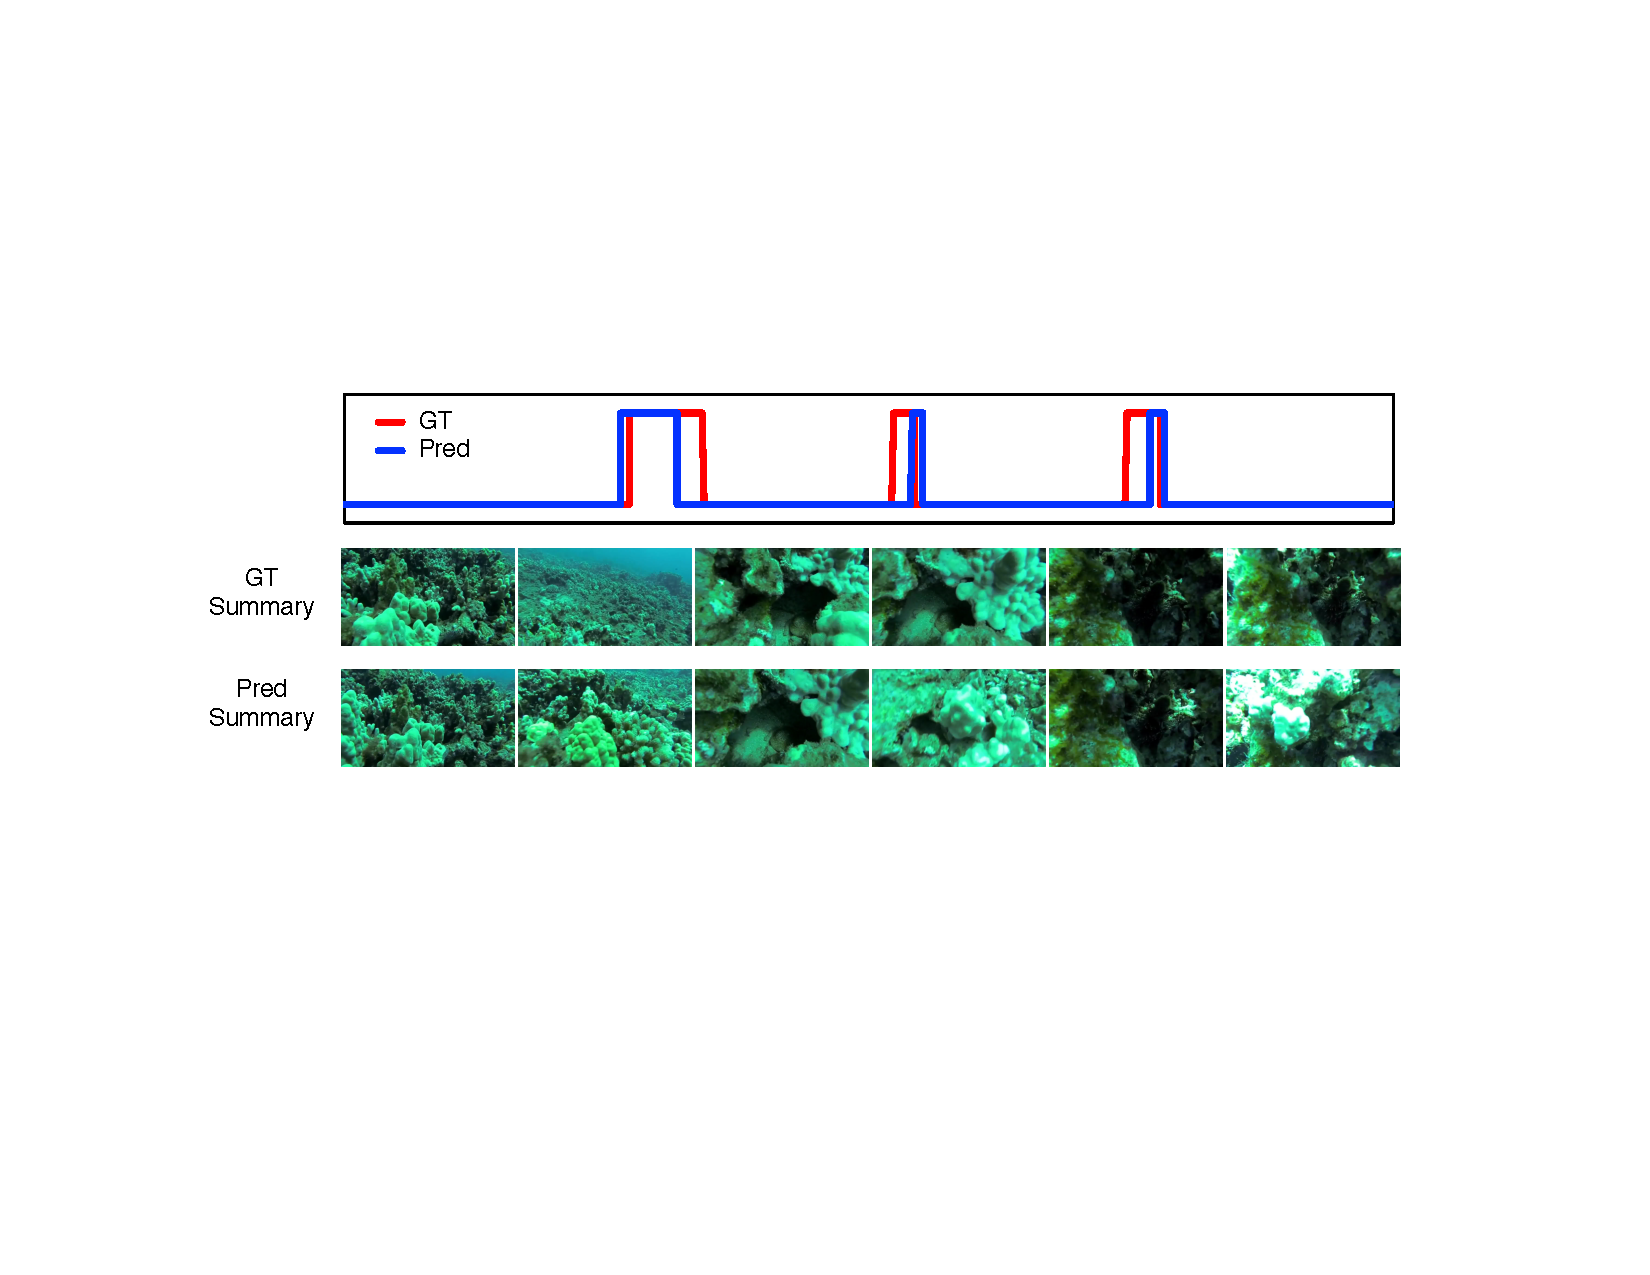
\includegraphics[width=\textwidth]{figures/vis_scub_v2.pdf}
    % \caption{Video of Scuba.}
   \end{subfigure} 
%       \begin{subfigure}[b]{\textwidth}
%   	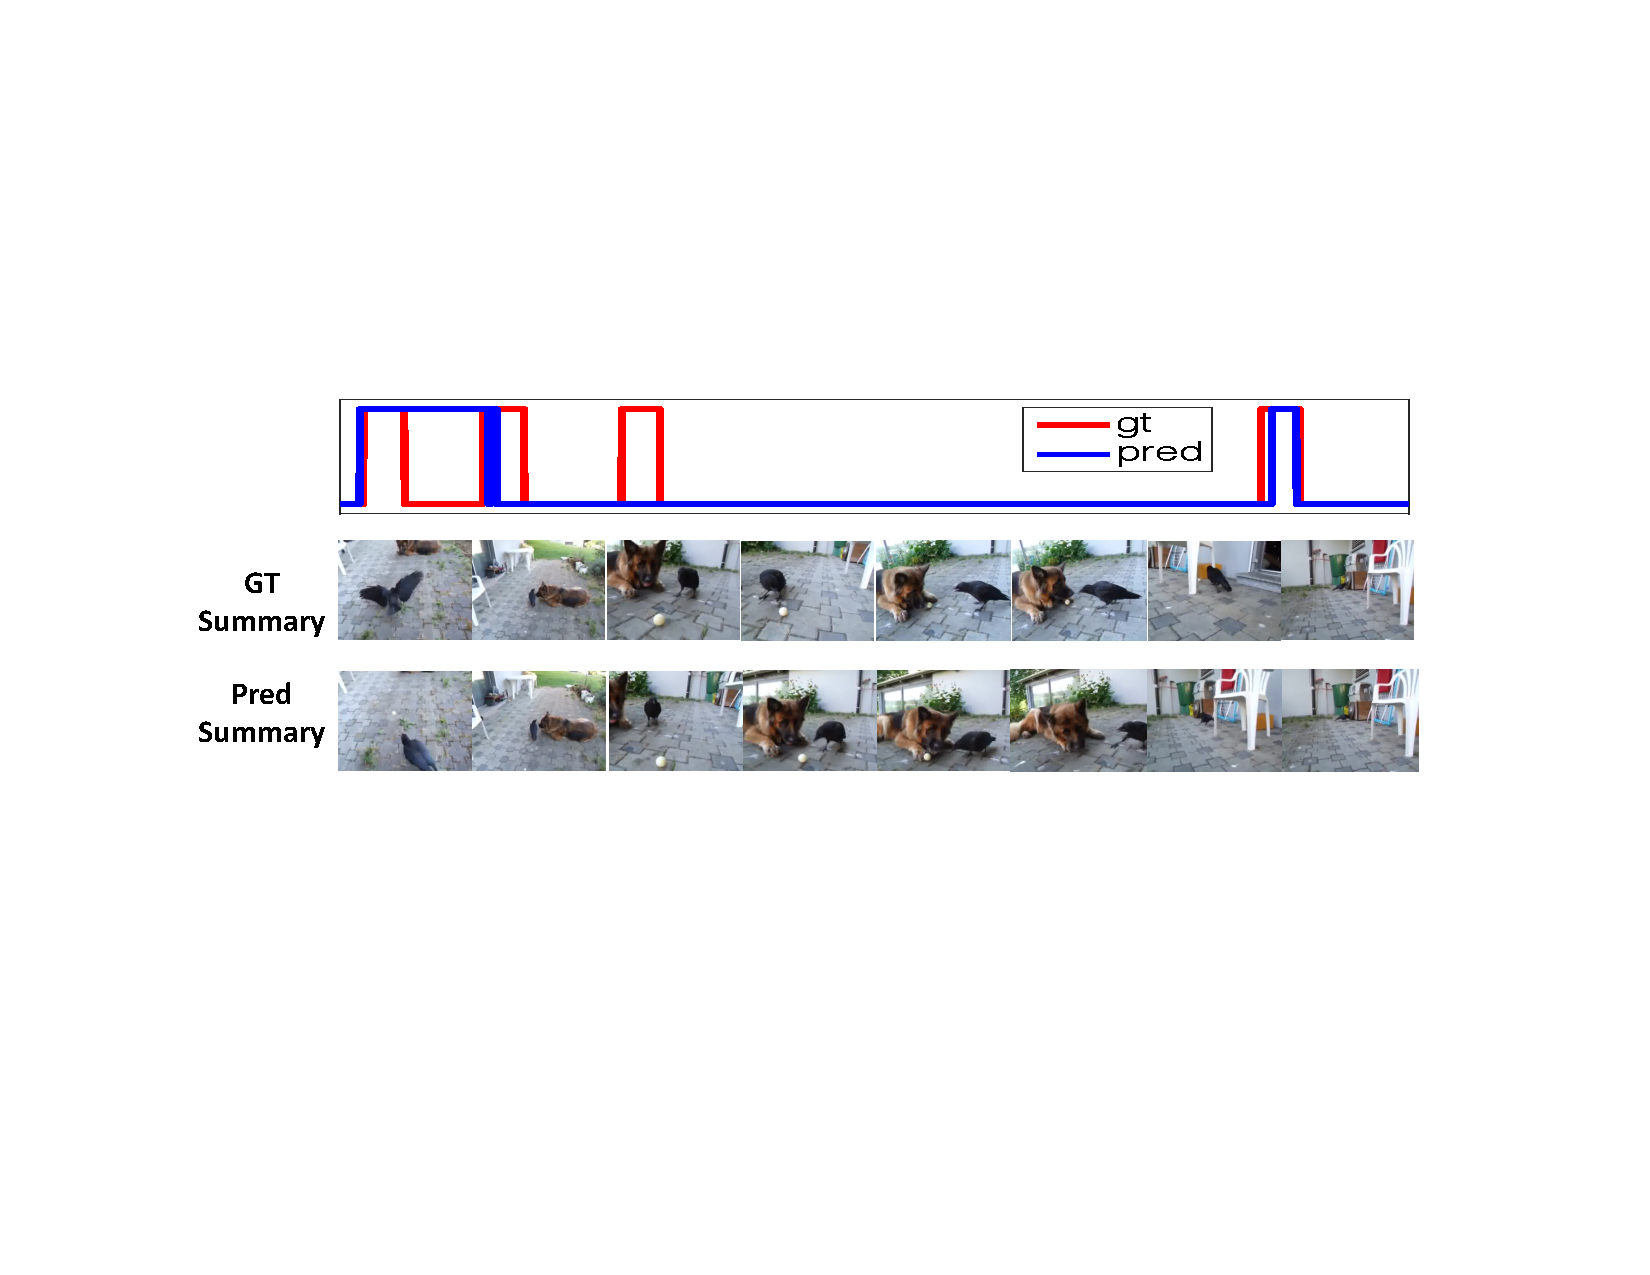
\includegraphics[width=\textwidth]{figures/vis_playball.pdf}
%     \caption{Video of Playing Ball.}
%   \end{subfigure} 
   \caption{ Visualization of the summarization results. \S2N localizes the interesting events in the video preferred by the annotators. \label{fig:vis_vs}}   
\vspace{-.05in}
\end{figure*}



\subsection{Temporal Action Proposal\label{sec:exp_THUMOS}}
Temporal Action Proposal (TAP) generation, akin to object proposal generation for images, is an important problem as accurate extraction of semantically important segments (e.g., human actions) from untrimmed videos is an important step for large-scale video analysis. Different than the previous applications, TAP aims for a slightly different goal, which to generate specific amount of high quality proposals that cover the action events with both high recall and high precision (based on temporal overlap). In this section we show that an \S2N can be trained to generate action proposals.


% Video action proposals generates temporal action proposals (segments) from long videos, which have contributed significantly to recent advances in temporal video action detection. 


\myheading{Dataset.} We evaluated \S2Ns on the THUMOS14 dataset~\cite{THUMOS14}, a challenging benchmark for the action proposal task. Following the standard practice, we trained an \S2N on the validation set and evaluated it on the testing set. On these two sets, 200 and 212 videos have temporal annotations in 20 classes, respectively. The average video duration in THUMOS14 is 233 seconds. The average number of labeled actions  in each video is around 15, making the task particularly challenging. The average action duration is 4 seconds and more than 99\% of the actions are within 10 seconds. We trained an \S2N using 180 out of 200 videos from the validation set and kept 20 videos for validation.
% Following the standard practice~\cite{zhao2017temporal} (\added[id=ZJ]{and more}), we train our models on the validation set and evaluate them on the testing set. On these two sets, 220 and 212 videos have temporal annotations in 20 classes. 

\myheading{Metrics}. We evaluated \S2N under the multiple metrics:

\begin{itemize}
	\item \textit{AR-N}~\cite{yu2015fast, lin2018BSN,escorcia2016daps,buch2017end}: this measures the average recall (AR) as a function of number of proposals per video. Note that the numbers of retrieved proposals ($N$) for all the test videos are the same regardless of their lengths. As AR-N was widely used in multiple previous works, in this paper we make it our primary metric. Additionally, following~\cite{Gao_2017_ICCV}, we also use the following metrics to further investigate the performance of \S2N.
	\item \textit{AR-F}~\cite{Gao_2017_ICCV}: this measures the average recall (AR) as a function of proposal frequency ($F$), which denotes the number of retrieved proposals per second for a video. For a video of length $L_i$ seconds and proposal frequency of $F$, the retrieved proposal number of this video is $N_i = F\times L_i$. 
	\item \textit{Recall@F-tIoU}~\cite{Gao_2017_ICCV}: this metric measures the recall rate at proposal frequency $F$ with regard to different tIoUs. In the evaluation, we set $F=1.0$ following~\cite{Gao_2017_ICCV}.
	\item \textit{Recall@N-tIoU}~\cite{Gao_2017_ICCV}: this metric measures the recall rate at number of retrieved proposals with regard to different tIoUs. 

\end{itemize}


%Additionally, following~\cite{Gao_2017_ICCV}, we also use the following metrics to further investigate the performance of \S2N:


\myheading{Features.} We used C3D features~\cite{tran2015learning}  to enable fair comparisons, as also used in~\cite{buch2017sst,escorcia2016daps}. We used activations from the top layer of a 3D convolutional network trained for action classification, then we performed PCA to reduce the dimensionality to improve computational performance in a similar fashion as~\cite{escorcia2016daps}.


% at 0.625 fps from the
% input videos.


% We use the two-stream I3D network [11] with architecture described in [35], where BN-Inception network [36] is used as
% temporal network and ResNet network [37] is used as spatial network. Two-stream network is implemented using Caffe [38] and pre-trained on ActivityNet-1.3 training
% set. 

\myheading{Implementation.}
We split each video into overlapping chunks of 360 frames (\textasciitilde 12s) and subsampled every 4 frames. We set the number of proposals generated from each chunk to be 15, which was the largest possible number of ground truth proposals contained in a chunk during training. 

During inference, we combined the proposals from chunks, sort them by their scores, and applied a Non-Maximum Suppression (NMS). This was the only post-processing step used to address the overlap introduced in splitting the videos. 

% We noted that in the inference stage, the X dose not 

\myheading{Baselines.}
% For exploring the effect of different assignment strategies and error diagnosis, we compare \S2N with TURN-C3D, which is a represenatitive algorithm that has the state of the art performances.
We first compare \S2N to the state-of-the art TAP generation methods including DAPs~\cite{escorcia2016daps} that uses an encoder LSTM and a regression branch for localization, Sparse-prop~\cite{caba2016fast} that applies dictionary learning for class independent proposal generation over a large set of candidate proposals, TURN-TAP~\cite{Gao_2017_ICCV} that evaluates candidate proposals in a sliding window manner over different temporal scales and level of contexts (we compare with variants of TURN-TAP based on different features and denote them as TURN-C3D and TURN-FLOW). We also compare with \textit{sliding window} and \textit{random} generators. For the DAPs, Sparse-prop, and TURN-TAPS, we plot the curves using the generated proposals provided by the authors. The sliding window proposals and random proposals are generated following Gao \etal~\cite{Gao_2017_ICCV}.

\begin{figure*}[t]
\centering
    
    \begin{subfigure}[b]{0.32\textwidth}
   	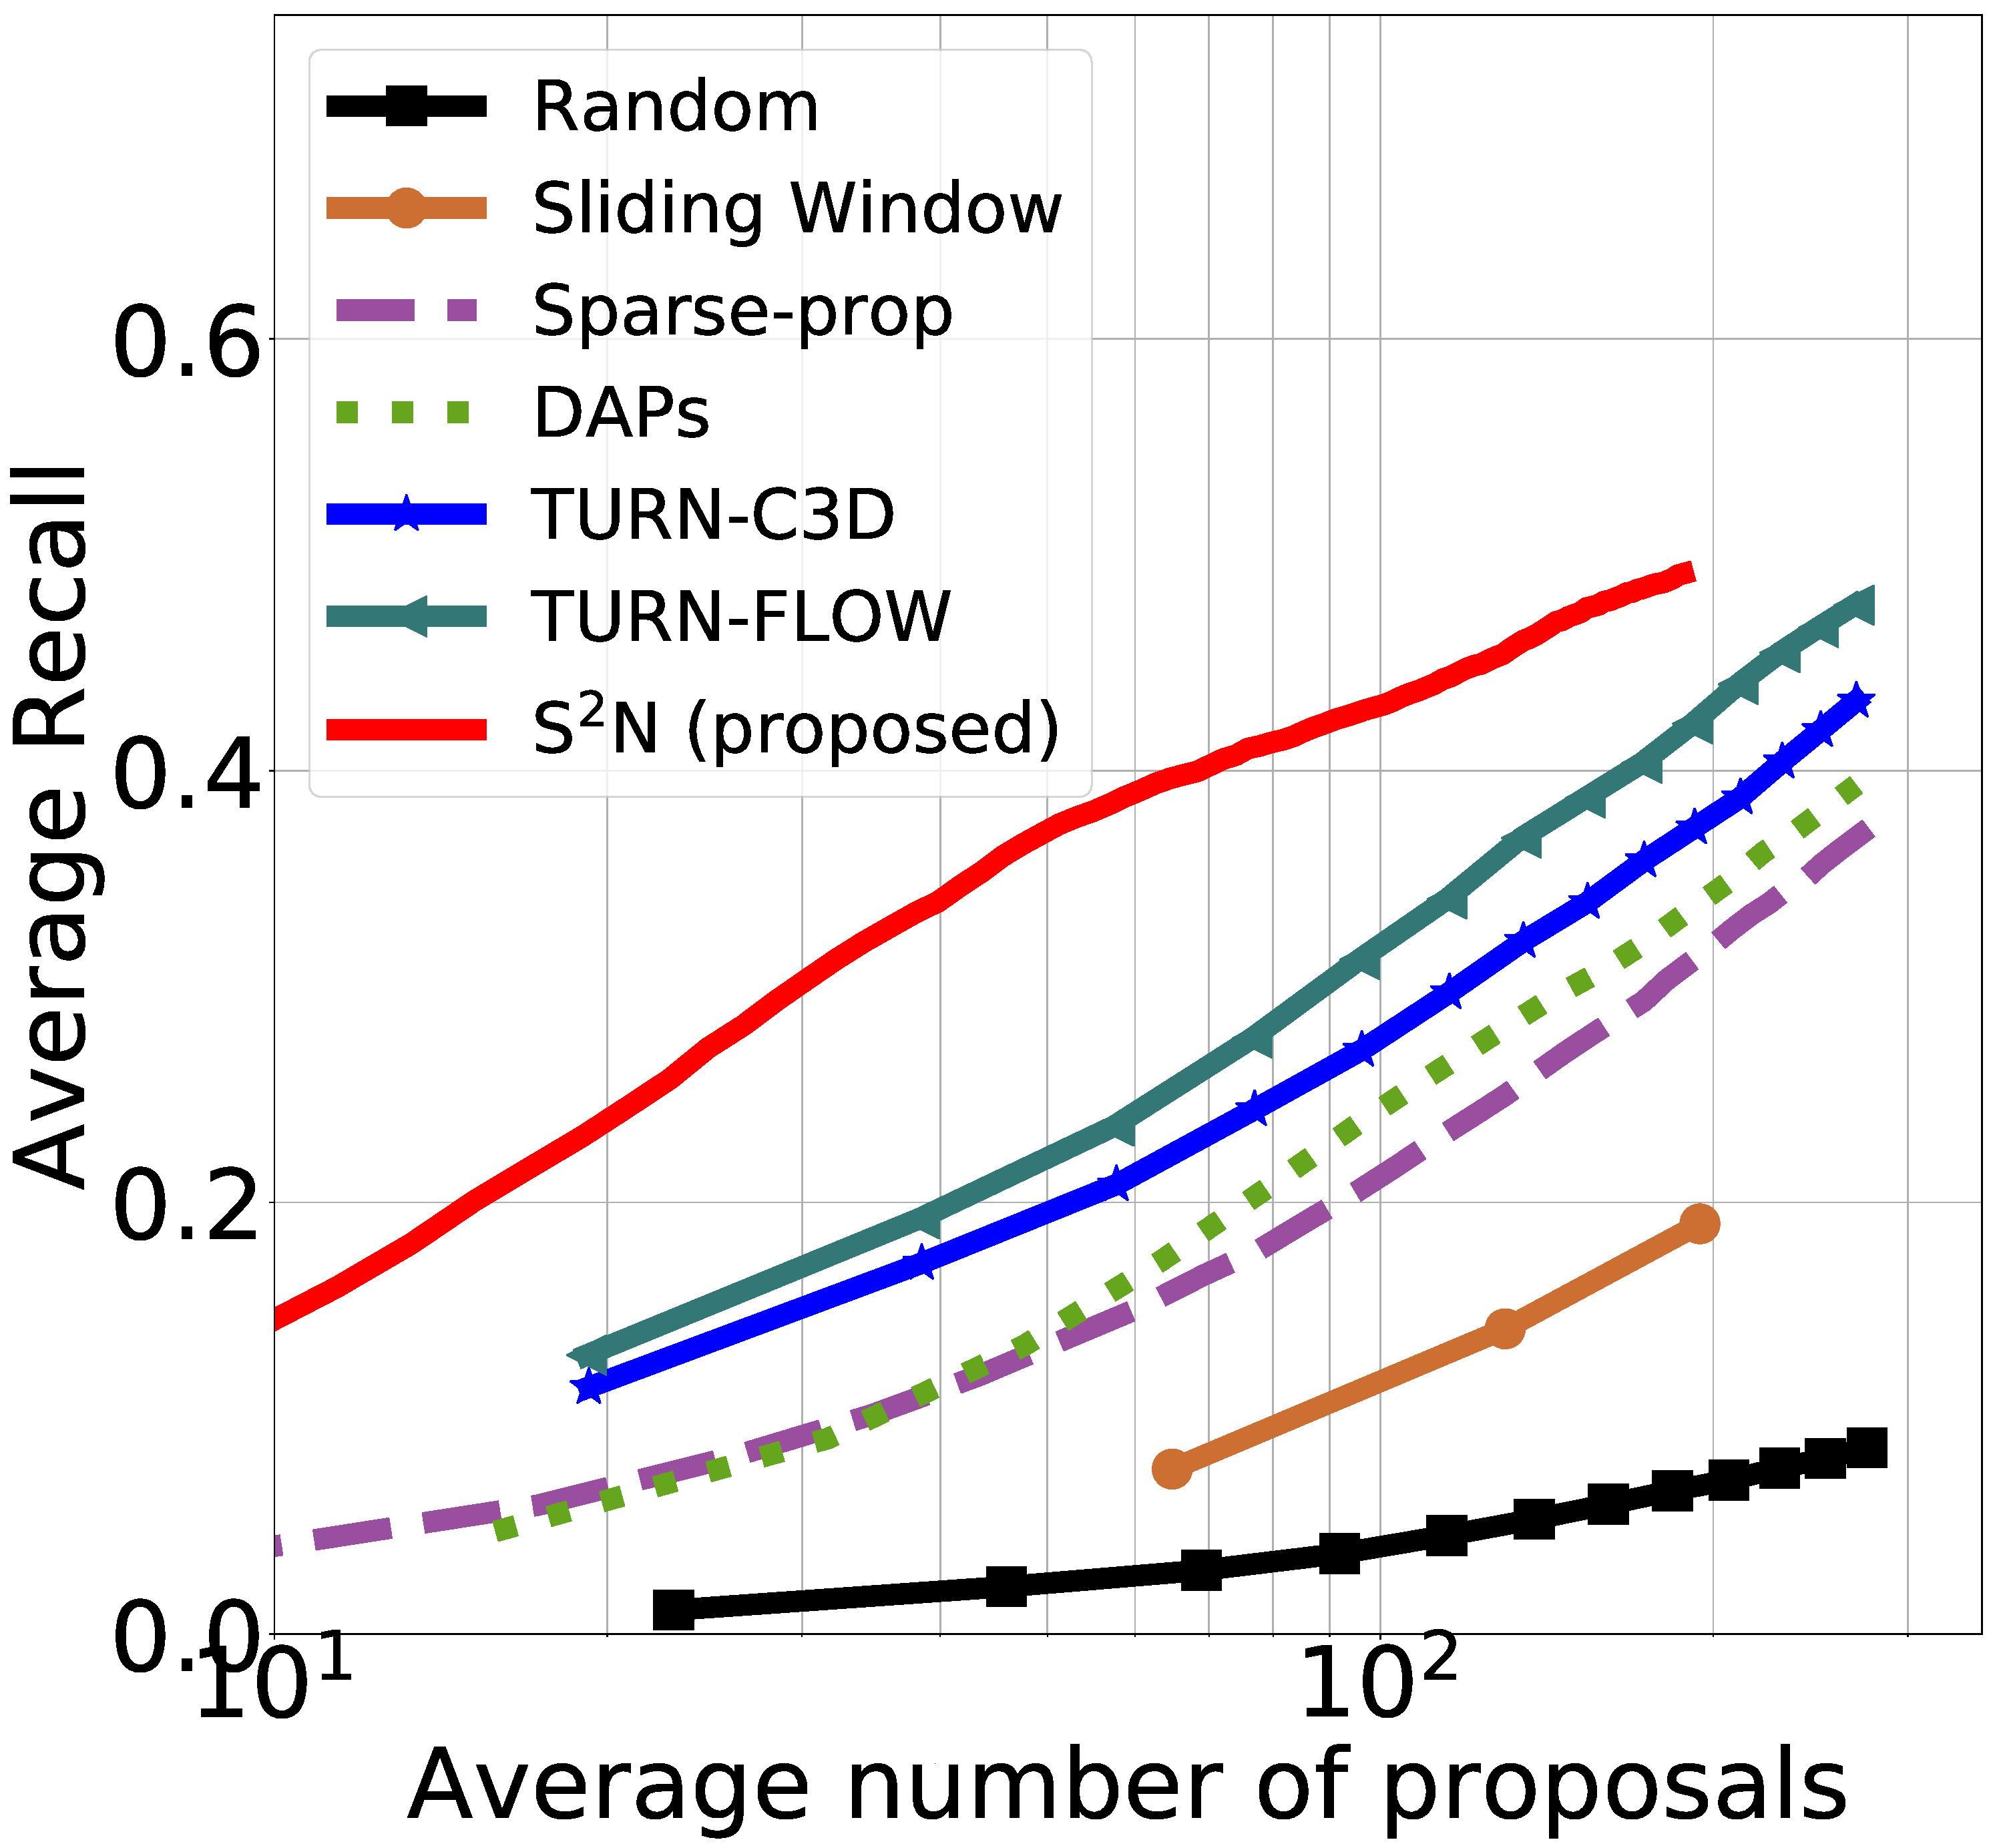
\includegraphics[width=\textwidth]{figures/results/Ours_avg_recall_pub.pdf}
    \caption{AR-N}
   	%\caption{easy cases}
   \end{subfigure}
   \begin{subfigure}[b]{0.32\textwidth}
   	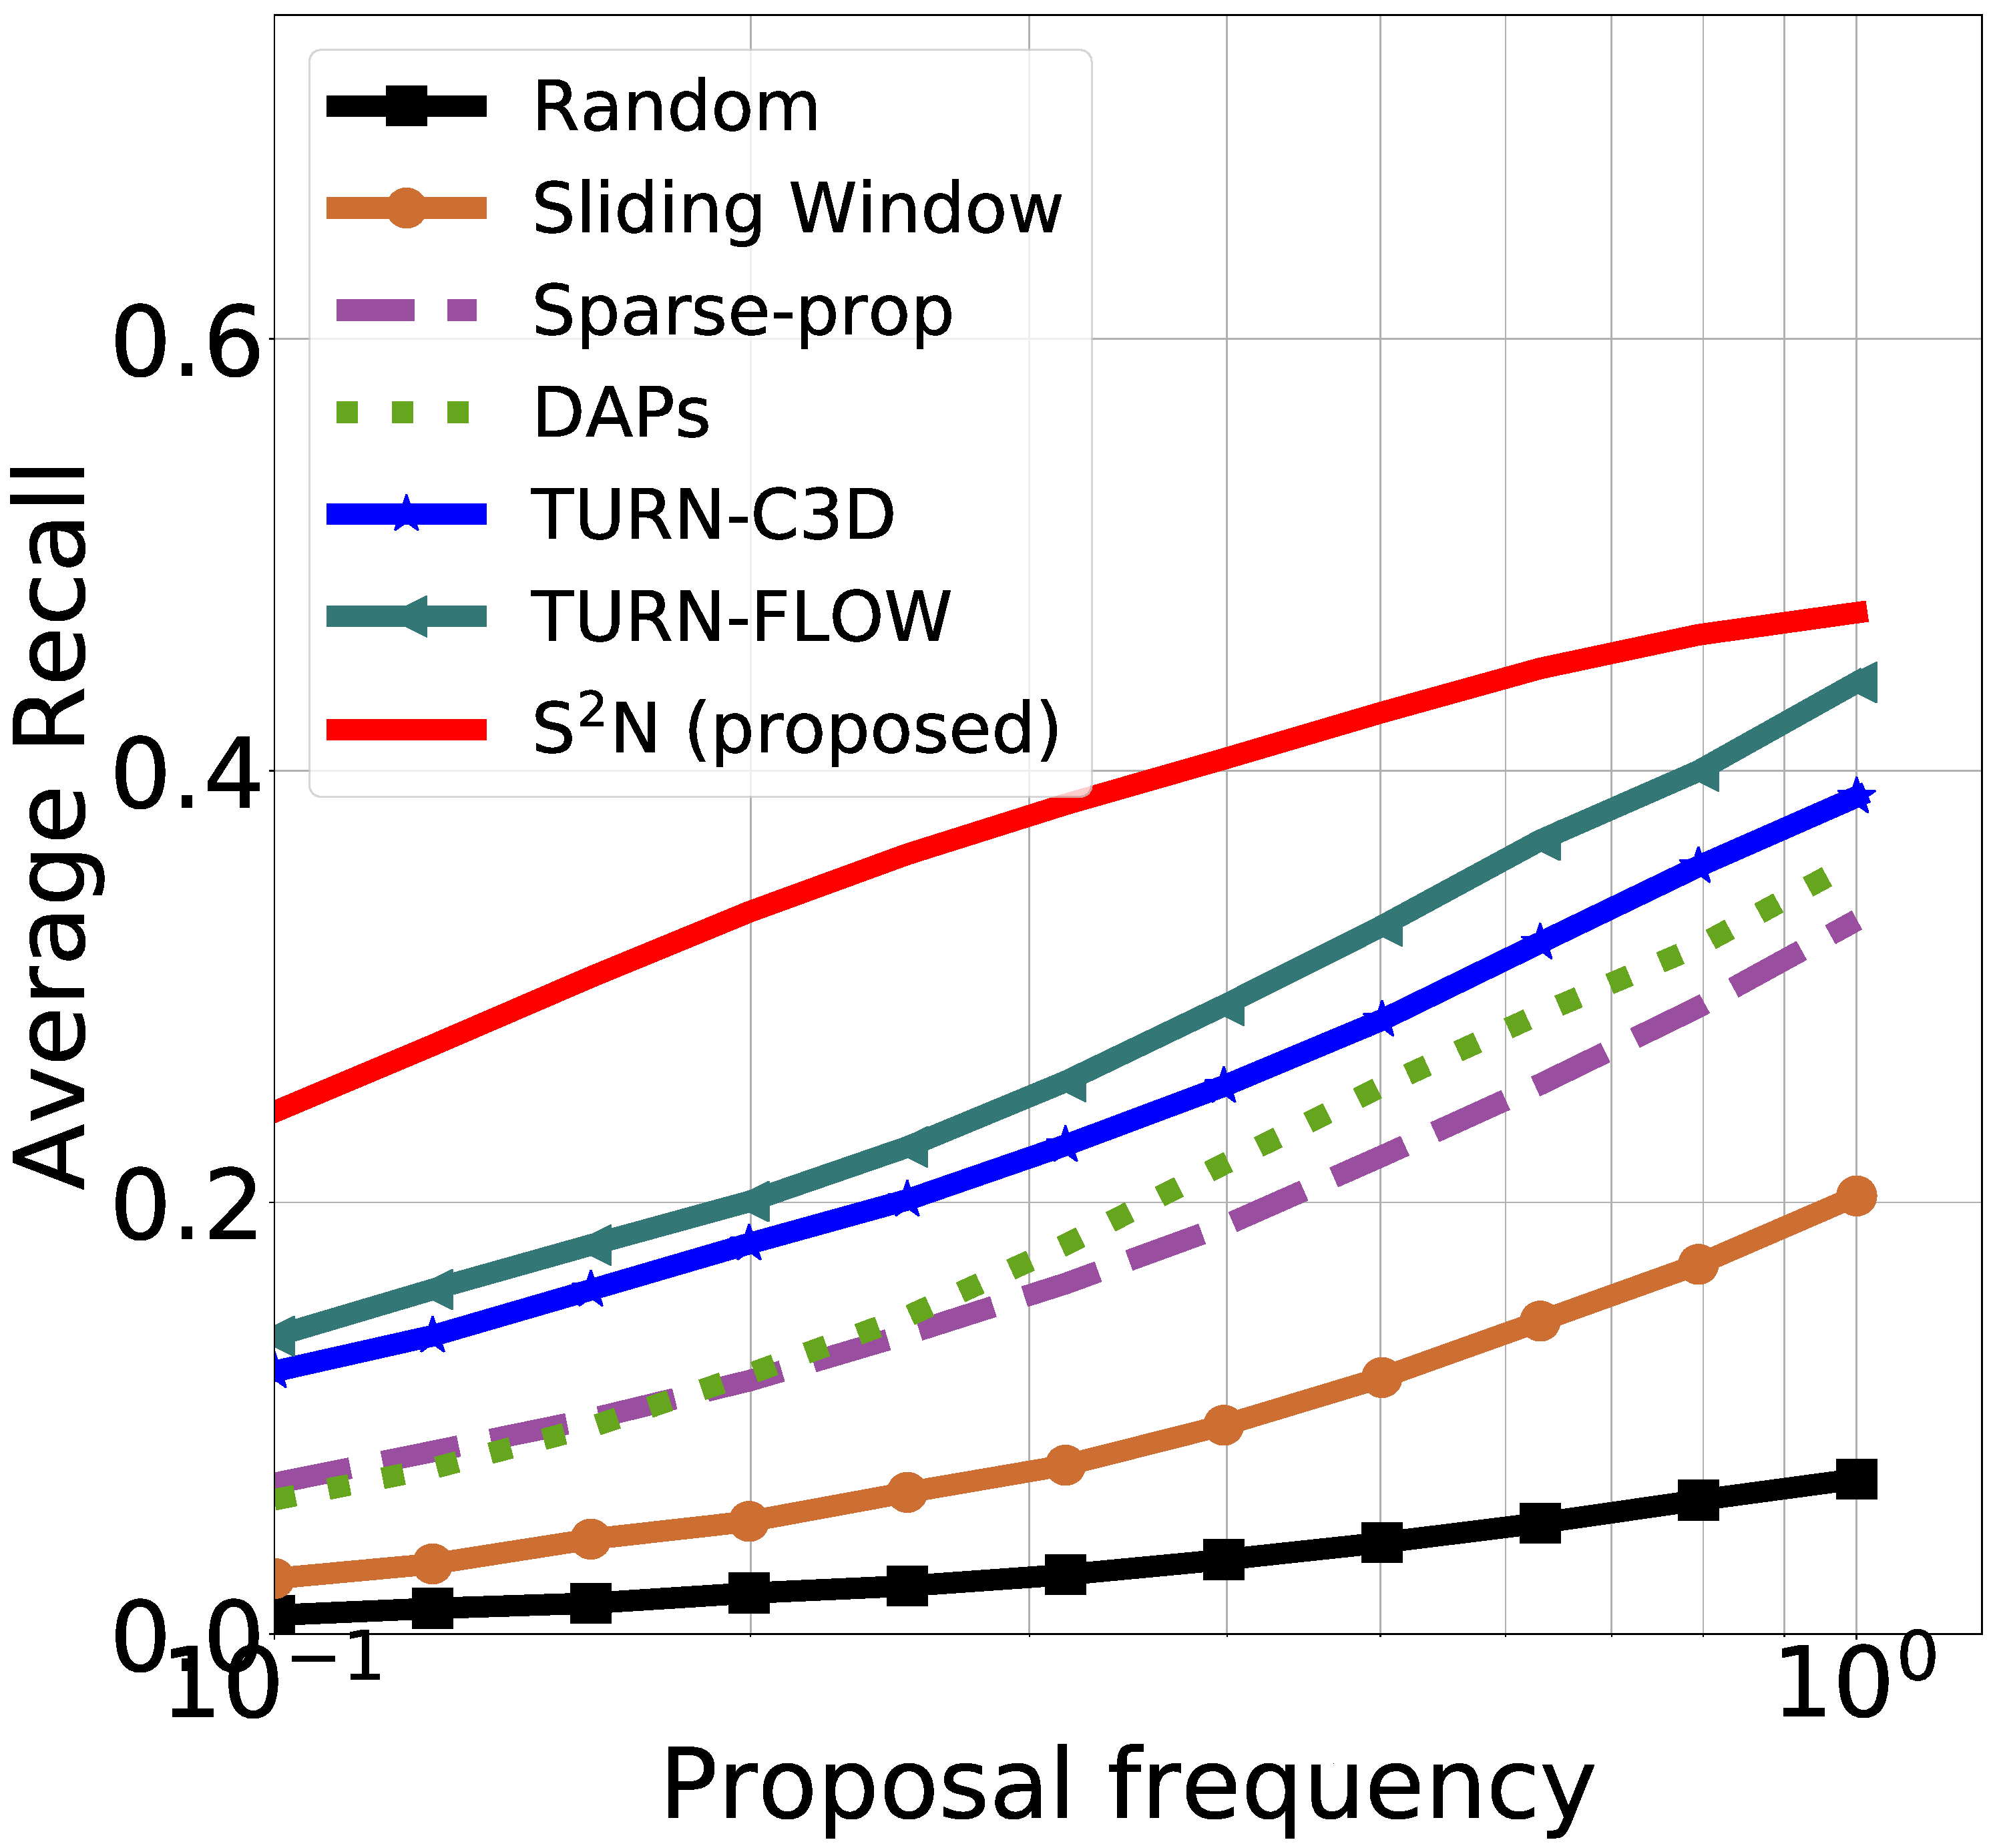
\includegraphics[width=\textwidth]{figures/results/Ours_freq_pub.pdf}
        \caption{AR-F}
   \end{subfigure}  
       \begin{subfigure}[b]{0.32\textwidth}
   	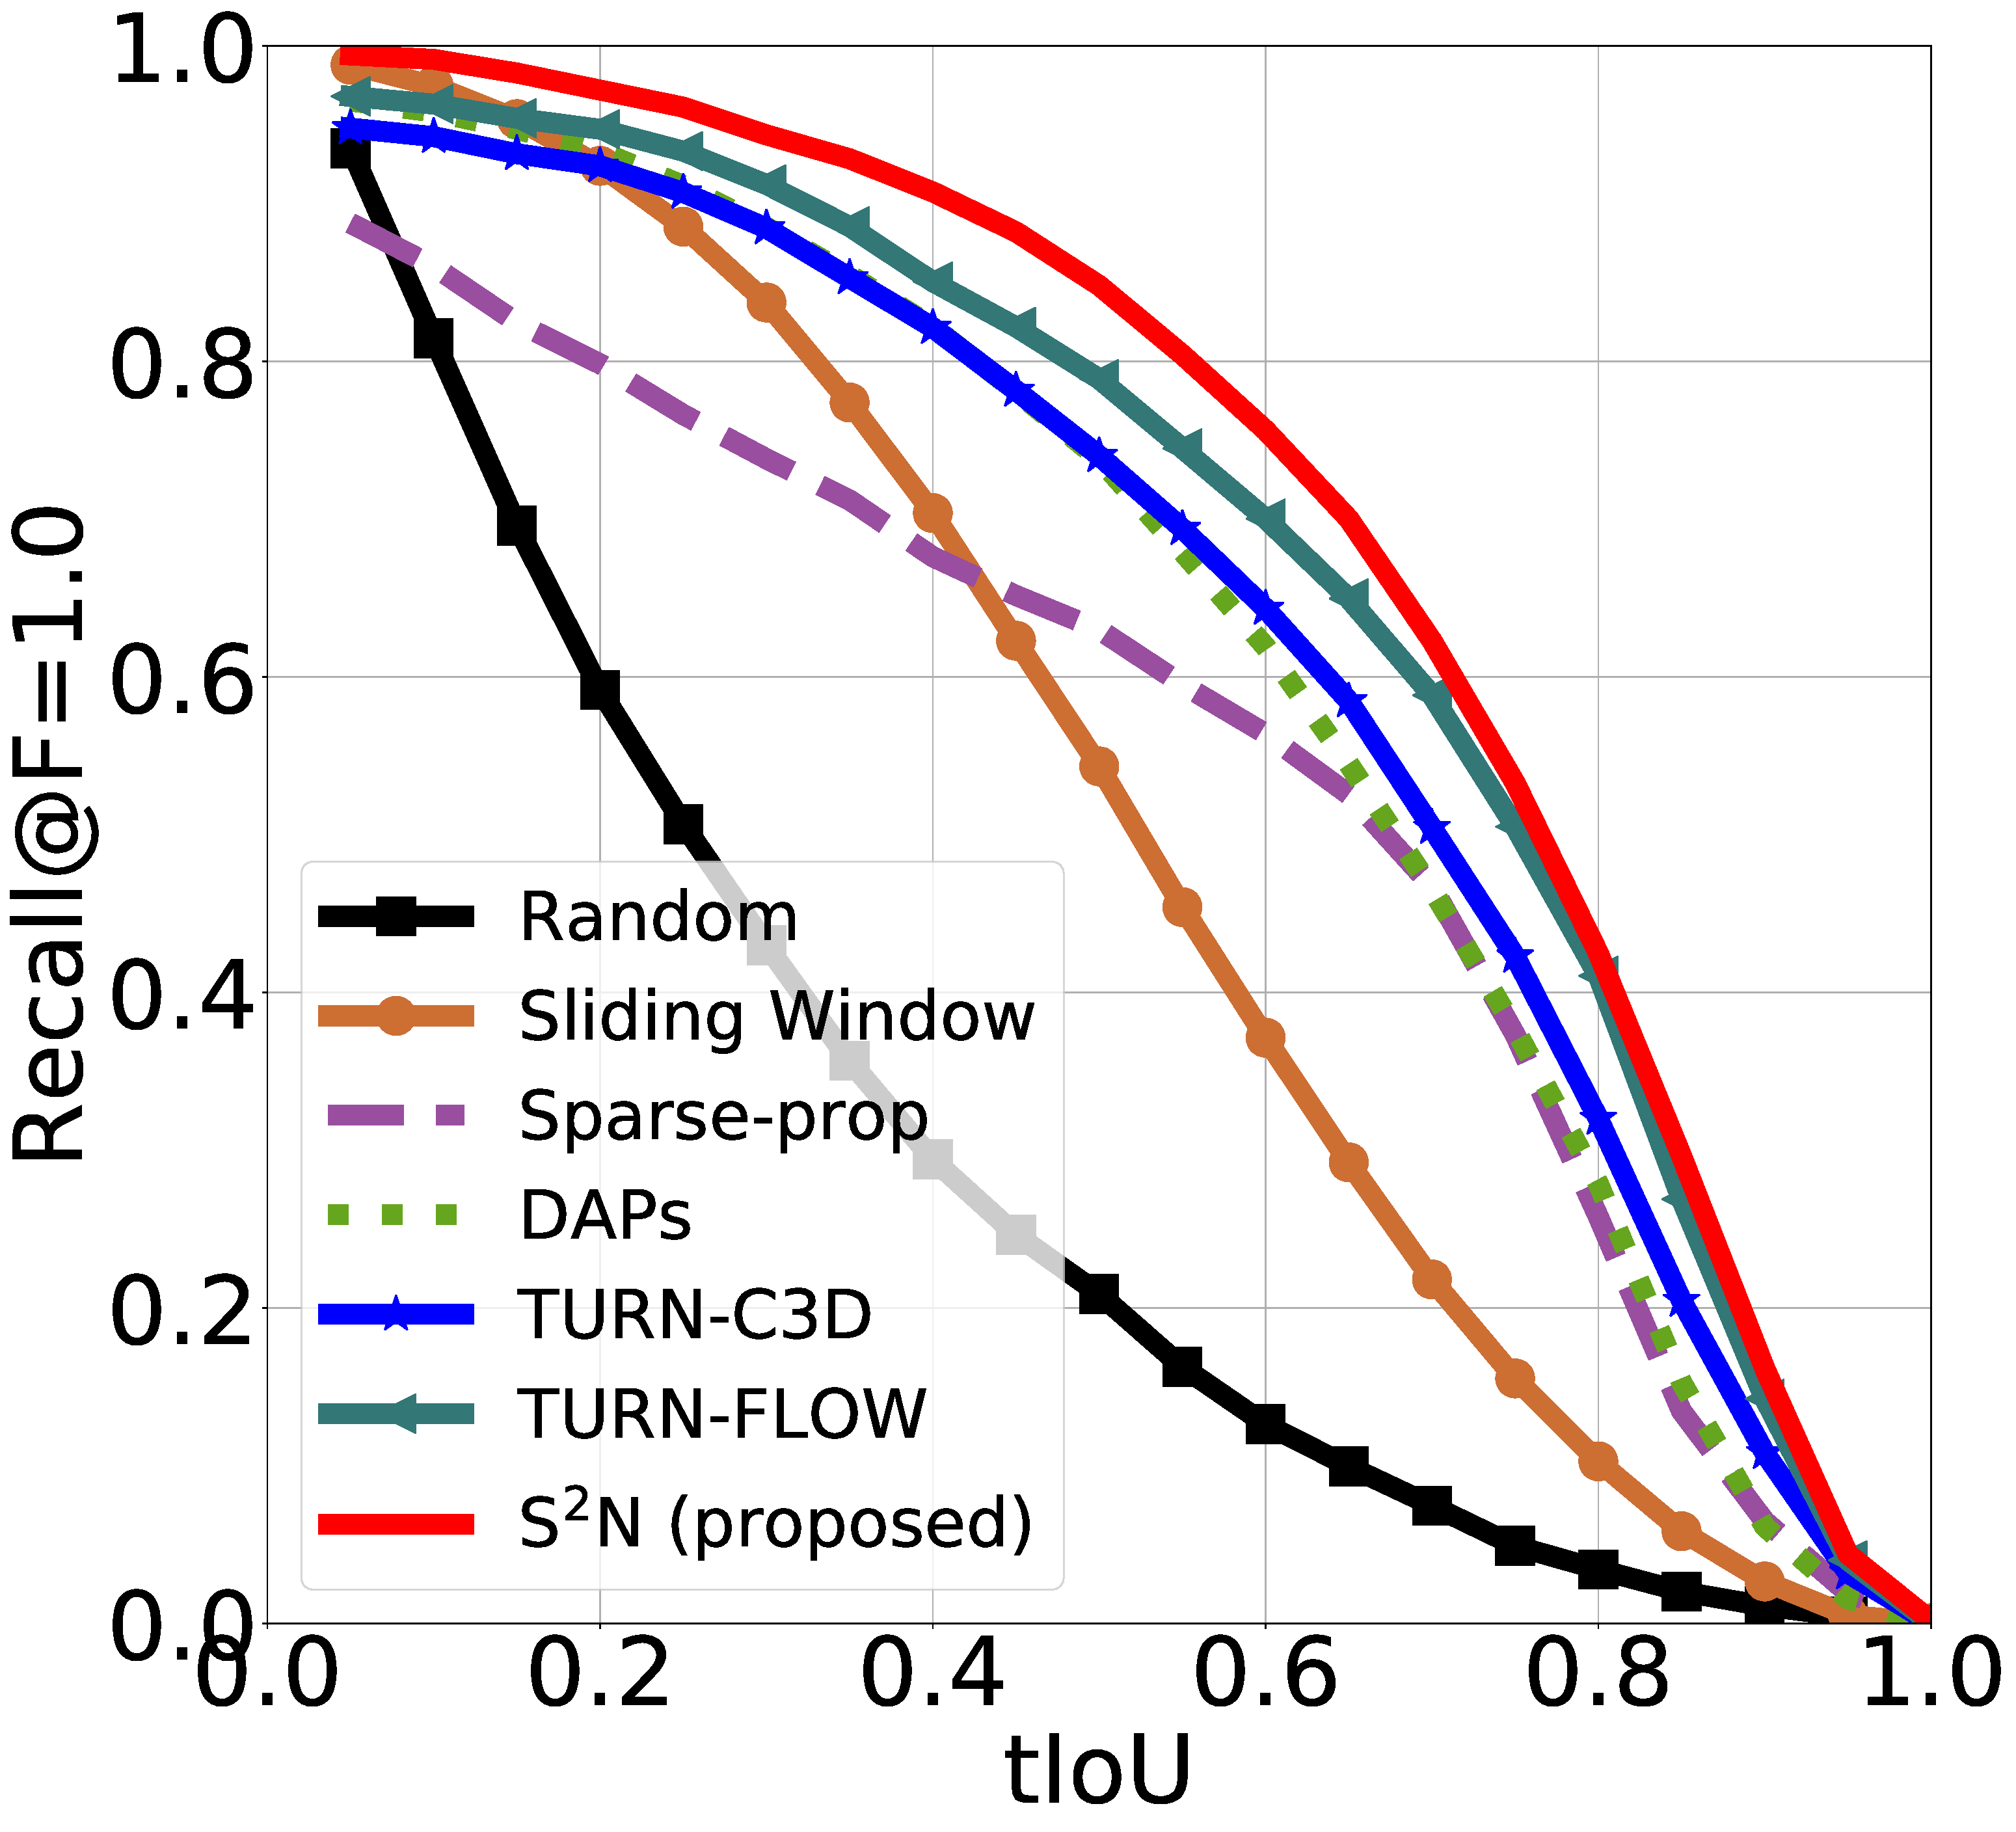
\includegraphics[width=\textwidth]{figures/results/Ours_recall_freq_pub.pdf}
    \caption{Recall@1.0-tIoU}
       \end{subfigure}  
%        \begin{subfigure}[b]{0.23\textwidth}
%    	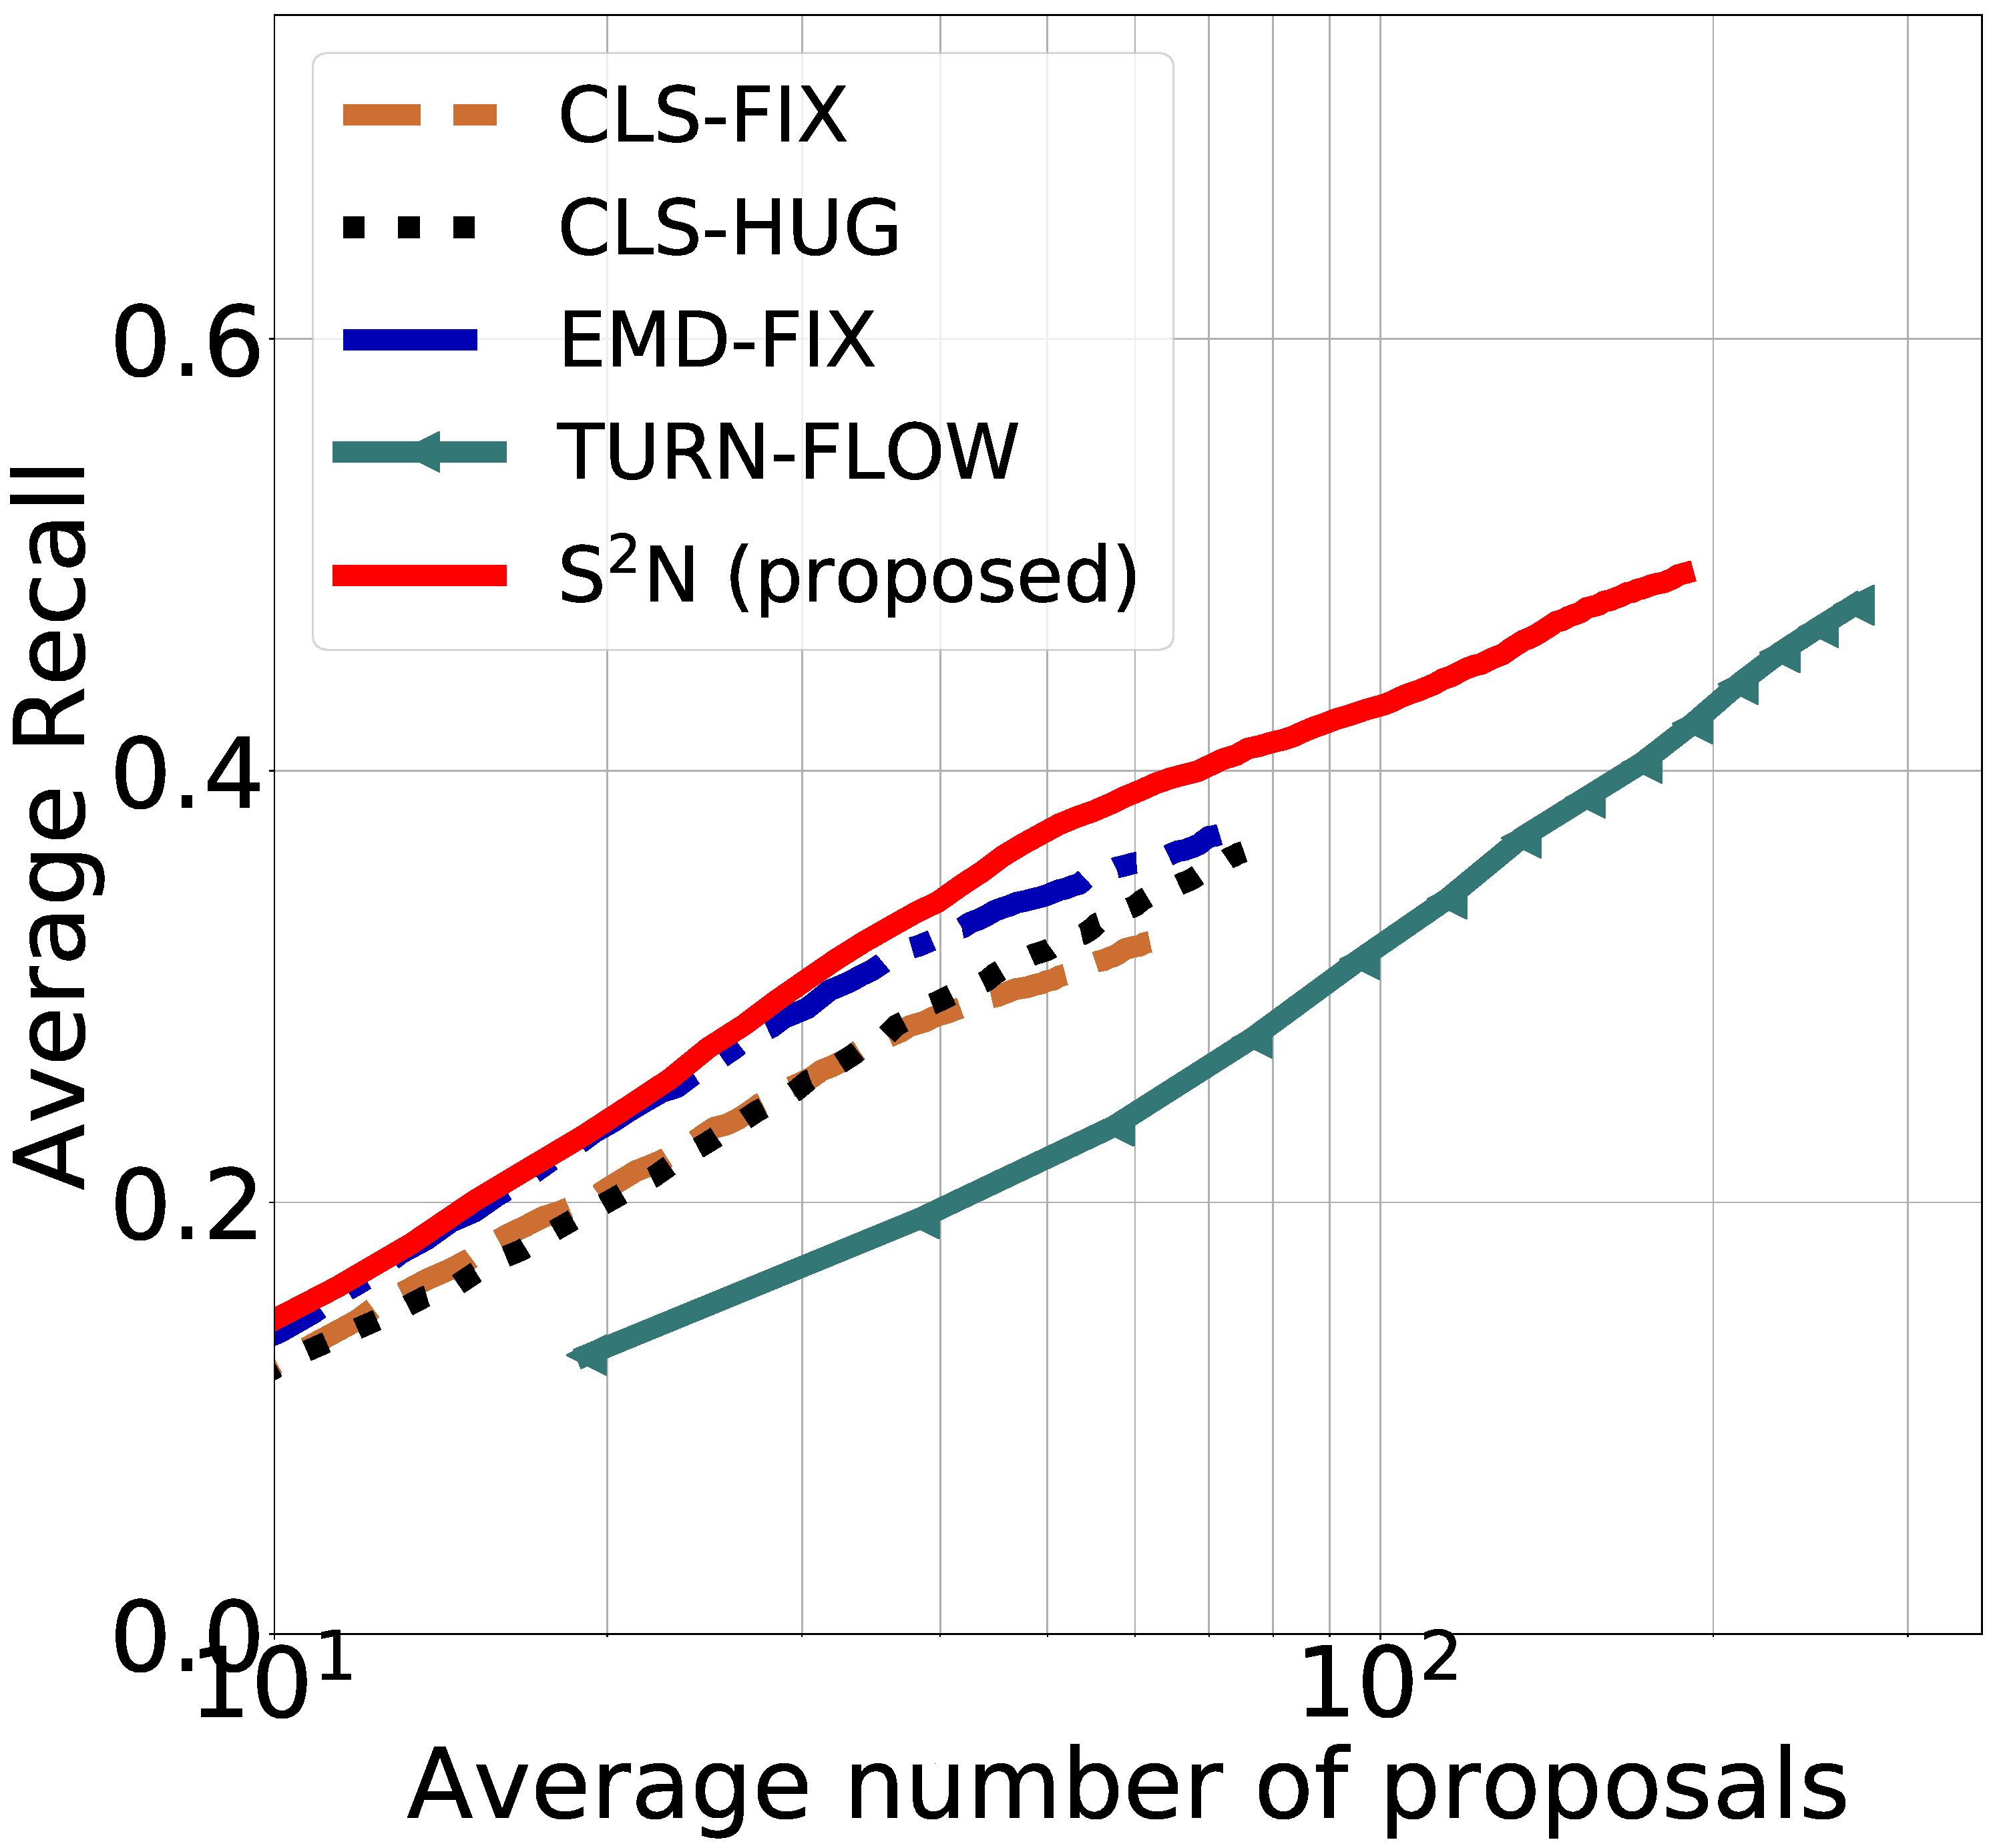
\includegraphics[width=\textwidth]{figures/results/Ours_avg_recall_comp.pdf}
% 	\caption{\label{subfig:avg-recall-comp}}
%    \end{subfigure}

   \caption{S2N with C3D features outperforms previous temporal and temporal action proposal generation approaches on THUMOS-14 under various performance metrics. \label{fig:proposal-c3d}}   
\vspace{-.05in}
\end{figure*}


\myheading{Results.} The performance of various methods under different metrics are shown in Figure~\ref{fig:proposal-c3d}. \S2N outperforms the other methods by a significant margin on all metrics. Note the gap between \S2N and DAPs partially implies the necessity of considering the contextual information. 


%}
\begin{figure}
\centering
\begin{subfigure}[b]{0.95\linewidth}
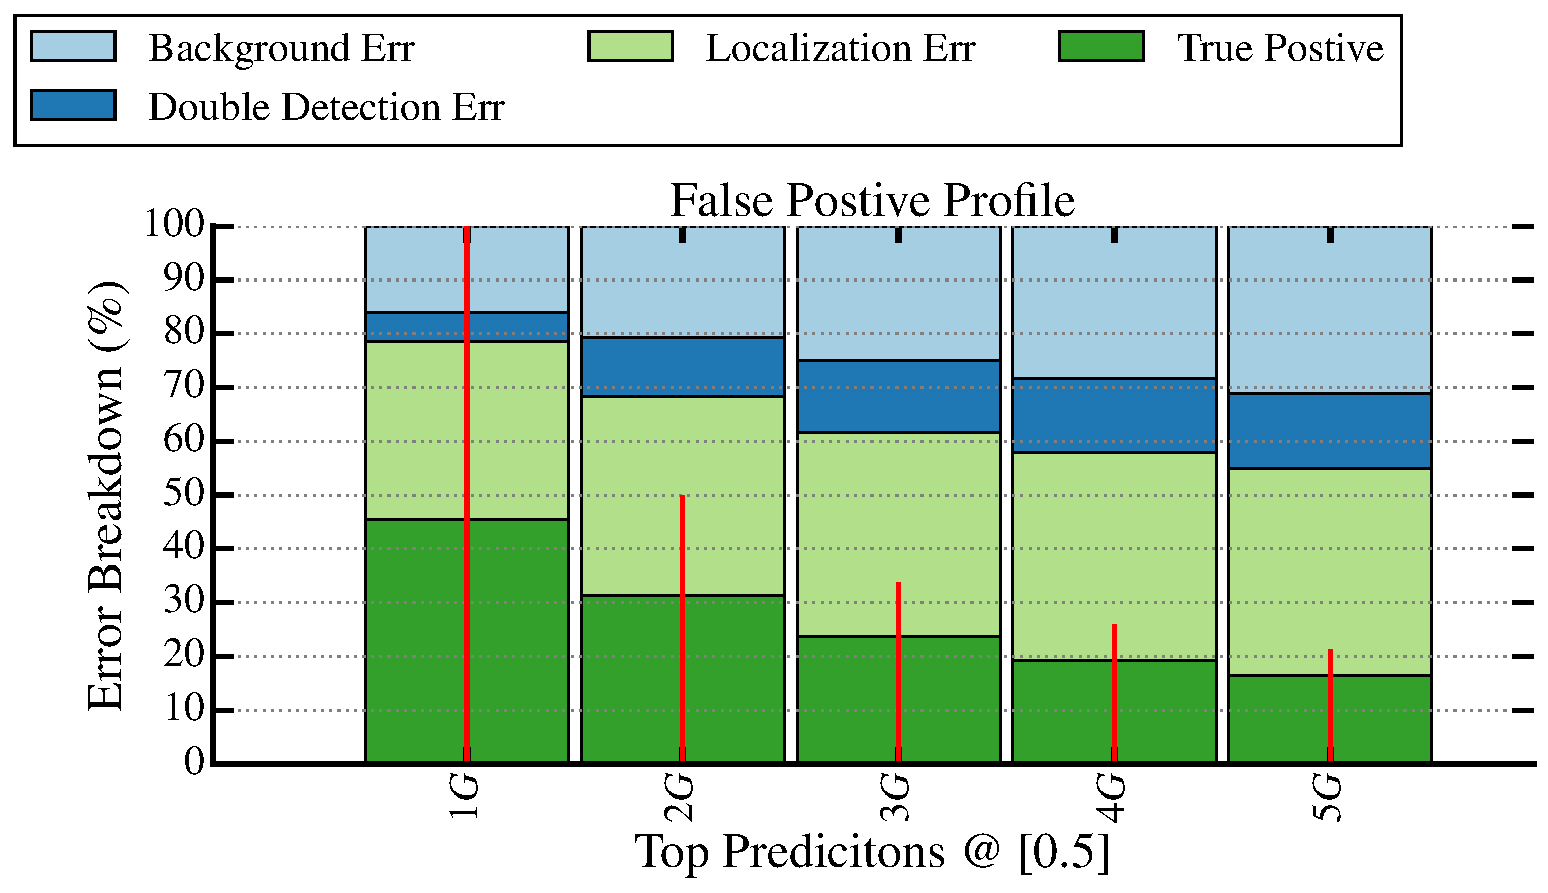
\includegraphics[width=\textwidth]{figures/ErrorDiag/false_positive_analysis-THUMOS14-EMD-HUG-0011-kG-tiou-05.pdf}
\vskip -0.05in
\caption{Error Analysis of \S2N with C3D features}
\end{subfigure}
\vskip 0.15in 
\begin{subfigure}[b]{0.95\linewidth}
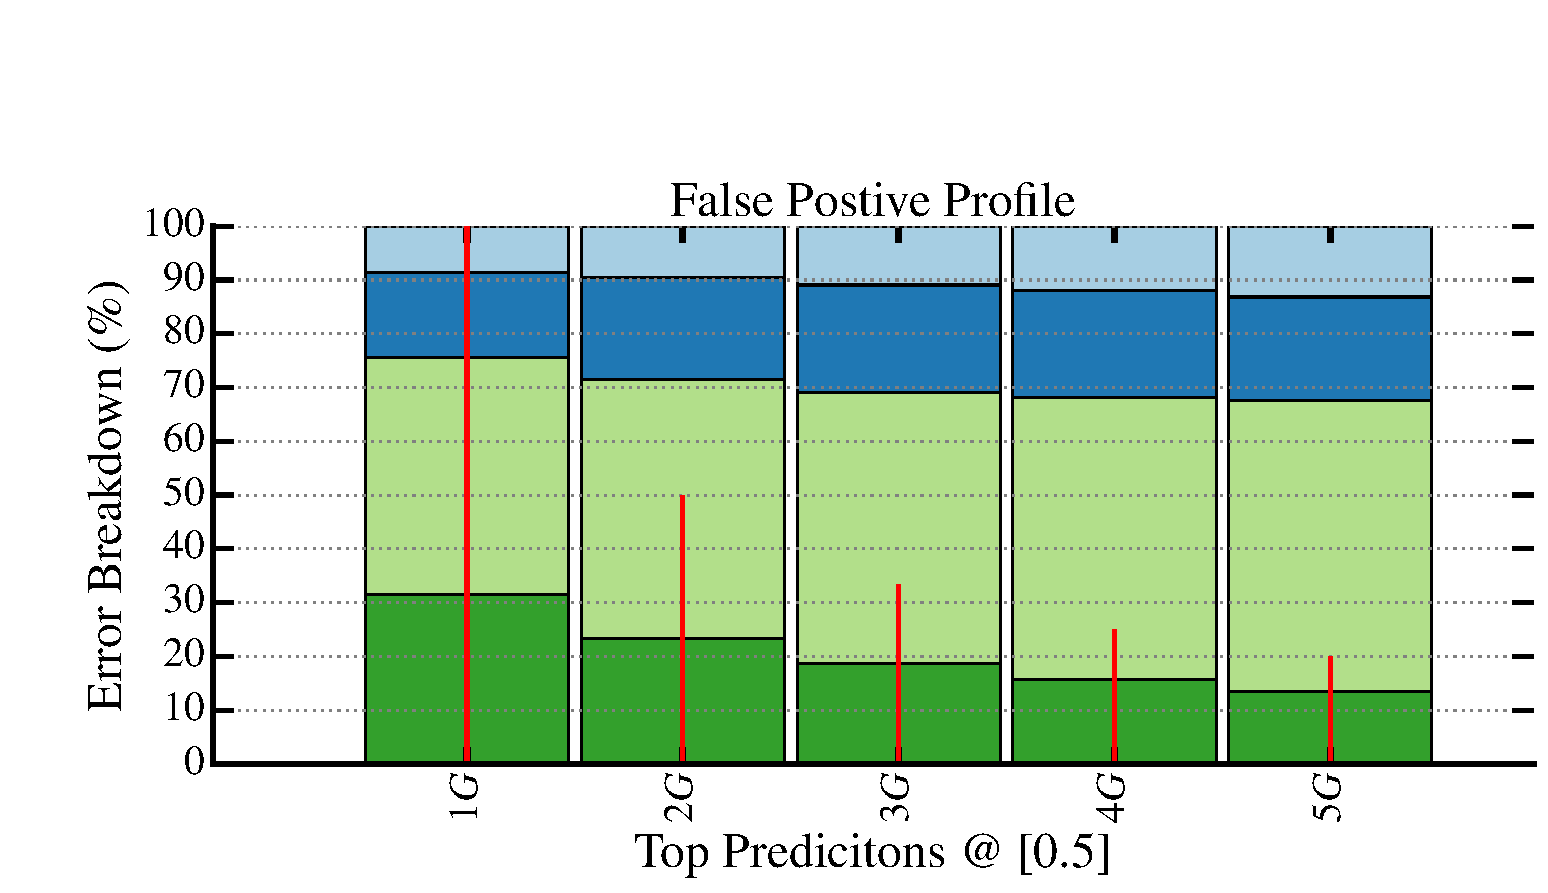
\includegraphics[width=\textwidth]{figures/ErrorDiag/false_positive_analysis-TurnC3D-kG-tiou-05.pdf}
\vskip -0.05in
\caption{Error Analysis of TURN-C3D}

\end{subfigure}
\caption{\label{fig:error-diag}Comparing different action proposal methods. Best viewed on a digital device.The red vertical lines indicate the number of true positives (100\% for 1G, 50\% for 2G ...)}
\end{figure}

\myheading{Diagnosing Error in Temporal Action Proposals}
To further investigate \S2N, we  performed some quantitative analysis~\cite{alwassel_2018_detad} to understand the types of errors often made by \S2N and how much each specific type of error affected the performance of the algorithm. 

Specifically, we followed the notions in Sec.~\ref{sec:loss_function}. A proposal $S_n$ was a \textbf{True Positive} if and only if $\exists G_m \in \mG$ such that $S_n$ was the highest scoring prediction with $tIoU(G_m, S_n)$ larger than a threshold. Otherwise, $S_n$ was a \textbf{False Positive} and we classified it into the following three categories: (1). \textit{Double Detection Error}: A prediction that satisfied the tIoU threshold with a ground truth instance, however, the ground truth instance had already been matched with another prediction of a higher score; (2). \textit{Localization Error}: A prediction that had a minimum 0.1 tIoU and failed to meet the tIoU threshold with the ground truth instance; (3). \textit{Background Error}: A prediction that did not meet a minimum 0.1 tIoU with any ground truth instance.

We executed our analysis on the error profile of the top-5G predictions, where G was the number of ground truth instances because 5G was already large enough for proposals of \S2N to cover most of the positives. We compared \S2N with C3D features to TURN-C3D~\cite{Gao_2017_ICCV} (one of the best competing methods), and the results are shown in Figure~\ref{fig:error-diag}. In addition to higher positive rate, we also note the following: (1) even with very limited number of proposals ($\leq 5G$), \S2N covered the majority of ground truth segments (around $90\%$); (2) the relatively smaller portion of double detection error and more back ground error showed that \S2N tended to produce more diverse results than its alternatives. 

\myheading{Speed.} \S2N is  efficient since it does not require repeated computation over multi-scale context. Specifically,  \S2N processes each frame in a sequence only once in the encoding stage and sequentially outputs multiple segments over the whole sequence in the decoding stage. It is more efficient than recent models (~\cite{buch2017sst,buch2017end}) that evaluate on a dense set of highly-overlapped candidates at each temporal step in a sequence. Quantitatively, it takes on average 0.028s to process a 12s, 30FPS video on a GTX Titan X Maxwell GPU with 12GB memory. In the batch mode,  it takes  around 2s to generate over 1200 proposals for an 8-minute video (14400 frames sampled every 4 frames). This is more than two times faster than the recently proposed models (1800 FPS \emph{v.s.} 701 FPS~\cite{buch2017end} \emph{v.s.} 308 FPS~\cite{buch2017sst} \emph{v.s.} 134 FPS~\cite{escorcia2016daps}).

% On numerical improvements are not enough to describe the whole picture. Further, we intend to answer the following
% questions: 
% \begin{enumerate}
%     \item How close are we to achieve our goal of delimiting the start and end of
% actions?
% \item What makes an algorithm more effective than another? What makes an
% action hard to localize?
% \item  Is the uncertainty of the temporal boundaries impeding
% the development of new algorithms? 
% \end{enumerate}



% \myheading{Results.} The comparison to baselines under \textit{AR-N}, \textit{AR-F},  and \textit{Recall@F=1.0-tIoU} metrics are shown in Figure~\ref{fig:proposal-c3d}. \S2N outperforms the baselines by a significant margin over all the metrics. Note the gap between \S2N and DAPs partially implies the necessity of considering the contextual information and the superiority of the proposed pointing mechanism.  Also note that we did not apply any post processing such as using the action length distributions as priors~\cite{shou2016temporal,Gao_2017_ICCV}, merging neighboring proposals or boundary refinement~\cite{shou2017cdc,Gao_2017_ICCV} other than a simple non-maximum suppression step. 

\begin{table*}
\setlength{\tabcolsep}{15pt}
\centering
\caption{Comparison between \S2N with other state-of-the-art proposal generation
methods on THUMOS14 in terms of Average Recall at N (AR-N). Methods based on I3D features outperform the ones based on C3D features. Using Beam Search also improves the overall performance. \label{results:proposal_ARAN}}
%\begin{tabularx}{\textwidth}{ X  X  X  X  X  X  X}
\begin{tabular}{llrrrrrr}	
\toprule
 Feature & Method & @50 & @100 & @200 & @500 &  @1000\\
\midrule
-        & Random & 2.47 & 4.44 & 7.42 & 13.09 & 16.11 \\
%-& Sliding Window & 5.33 & 9.32 & 16.28& 33.22 & 49.22 \\
\midrule
C3D &  DAPs~\cite{escorcia2016daps} & 13.56 & 23.83 & 33.96 & 49.29 & 57.64 \\
C3D & SCNN-prop~\cite{caba2016fast} & 17.22 & 26.17 & 37.01 & 51.57 & 58.20 \\
C3D & TURN~\cite{Gao_2017_ICCV} & 19.63 & 27.96 & 38.34 & 53.52 & 60.75\\
C3D & BSN + Greedy-NMS ~\cite{lin2018BSN} & 27.19 & 35.38 & 43.61 & 53.77 & 59.50 \\
C3D & BSN + Soft-NMS~\cite{lin2018BSN} & 29.58 & 37.38 & 45.55 & 54.67 & 59.48 \\
\midrule
C3D & \S2N  & 37.06 & 43.04 & 49.18 & - & - \\
C3D & \S2N-Beam  & \textbf{36.80} & \textbf{44.23} & \textbf{52.11} & \textbf{59.59} & \textbf{64.46} \\
\midrule
Flow & TURN~\cite{Gao_2017_ICCV}  & 21.86 & 31.89 &  43.02 &  57.63 & 64.17 \\
%\midrule
Two-stream~\cite{Simonyan-Zisserman-NIPS14} & TAG~\cite{zhao2017temporal} & 18.55 & 29.00 & 39.61 & - & - \\
Two-stream~\cite{xiong2016cuhk} & BSN + Greedy-NMS~\cite{lin2018BSN} & 35.41 & 43.55 & 52.23 & 61.35 & 65.10 \\
Two-stream~\cite{xiong2016cuhk} & BSN + Soft-NMS~\cite{lin2018BSN} & 37.46 & 46.06 & 53.21 & 60.64 & 64.52 \\
%\midrule
%2-Stream & BSN + Greedy-NMS~\cite{lin2018BSN} & 35.41 & 43.55 & 52.23 & 61.35 & 65.10 \\
I3D~\cite{carreira2017quo} & \S2N-Beam & \textbf{41.29} & \textbf{51.96} & \textbf{59.19} & \textbf{66.01} & \textbf{69.11} \\
\bottomrule
%\end{tabularx}
\end{tabular}
\setlength{\tabcolsep}{0.1cm}
%\vskip -0.1in
\end{table*}

\subsection{Improving \S2N for Temporal Action Proposal\label{sec:improved-S2N-exp}}

In this section, we will describe several techniques to further advance the performance of the \S2N. In particular, we will replace C3D features by the better and more recent I3D features~\cite{carreira2017quo}, and we introduce beam search to extend the recall range of the method.

\myheading{Using more sophisticated features.} So far, we have used \S2Ns with C3D features, so the resulting \S2N models are directly comparable to other existing methods that also used C3D features. As we have shown in the previous section, \S2Ns with C3D features have achieved the state-of-the-art performance, outperforming other methods. However, the underlying C3D features are no longer the state-of-the-art for human action recognition; there are more recent and advanced features such as I3D~\cite{carreira2017quo}. In this section, we experiment \S2N with I3D, aiming to advance the state-of-the-art performance even further. I3D~\cite{carreira2017quo} is a two-stream model that is built upon image classification architectures~\cite{szegedy2015going} where filters and inflated from 2D to 3D, leading to very deep, naturally spatio-temporal models. We used the  same model of~\cite{carreira2017quo} pre-trained on the Kinetics dataset~\cite{kay2017kinetics} for action classification. This model inputs a stack of 64 RGB/optical flow frames and extracts a 1024-dimensional feature vectors. We extracted both RGB and optical flow features for each frame.  We then performed PCA to reduce the dimensionality. The input to \S2N is the concatenation of  two 500-dimensional feature maps. 

\myheading{Extending the range of recall values with beam search.} 


%\red{Need to explain this problem better. Why does it only generate a  limited number of proposals?}
One caveat of \S2N is that it only generates a limited number of proposals (generally $\leq 300$). This is because in training, over different iterations, detections from different decoding steps might be assigned to the same ground truth, based on the HMLC strategy. However, HMLC only penalizes the offsets of the detections that are matched with ground truth, there is no penalty forcing the false positives to be far away from the true positives. The matching and the loss function cause \S2N to output repetitive detections that maximally covers the target segments (an example is shown in Fig.~\ref{fig:HMLC_r3}).  This is fine for tasks such as video highlighting or video summarization tasks. However, it makes \S2N less competitive for temporal action proposal tasks in which more proposals are allowed. 
To address the problem of generating insufficient proposals, during inference we propose a simple but effective modification by using \emph{Beam Search}: for each decoding step, instead of only generating one proposal $S_n$ from the maximum response locations(Eq.~\ref{eqn:eq1}), here we make \S2N to N proposals from the top N maximum response locations. The score in a $S_n = (b_n, d_n, c_n)$, which previously was only determined by the output of the score predictor branch (Sec.~\ref{sec:SDU}) is now a product of the score predictor and the response scores for the starting and ending position, \emph{i.e.}:
\begin{equation}
    \Bar{c}_n = c_n \cdot \sigma (g (\h_n, \e_{b_n})) \cdot \sigma(g(\h_n, \e_{d_n}))
\end{equation}
where $g(\cdot, \cdot)$ is defined in Eq.~\ref{eqn:eq2} and $\sigma(\cdot)$ is the softmax function.

In this way, we can generate N times more proposals than previous \S2N. We denote \S2N with this modification as \emph{S2N-Beam}. We fix N to 10 for all the experiments.


\myheading{Results.} 
Table~\ref{results:proposal_ARAN} shows a complete comparison between variants of \S2N and the current state-of-the-art algorithms under the AR-N metric. In addition to the set of baselines described in Sec.~\ref{sec:exp_THUMOS}, we also include Boundary-Sensitive Network (BSN)~\cite{lin2018BSN}, a recently published multiple-stage pipeline that detects boundaries and groups them as proposals. As shown in Table~\ref{results:proposal_ARAN}, with the same features, the \S2N methods significantly outperform the others. Notably, on average the \S2N-Beam with I3D features surpasses the BSN method by 5 percent.

Figure~\ref{fig:proposal-2stream} plots the entire performance curves of several methods: BSN, S2N-C3D, S2N-Beam-C3D, and S2N-Beam-I3D. In addition to the performance curves under the AR-N metric (Figure~\ref{fig:proposal-2stream}a), this figure also shows the performance curves under other metrics: AR-F, Recall@F-1.0 and Recall@N=1000. As shown in figure, using beam search (\S2N-Beam) improves performance especially when proposal frequency is high.


\begin{figure*}[t]
\centering
    
    \begin{subfigure}[b]{0.24\textwidth}
   	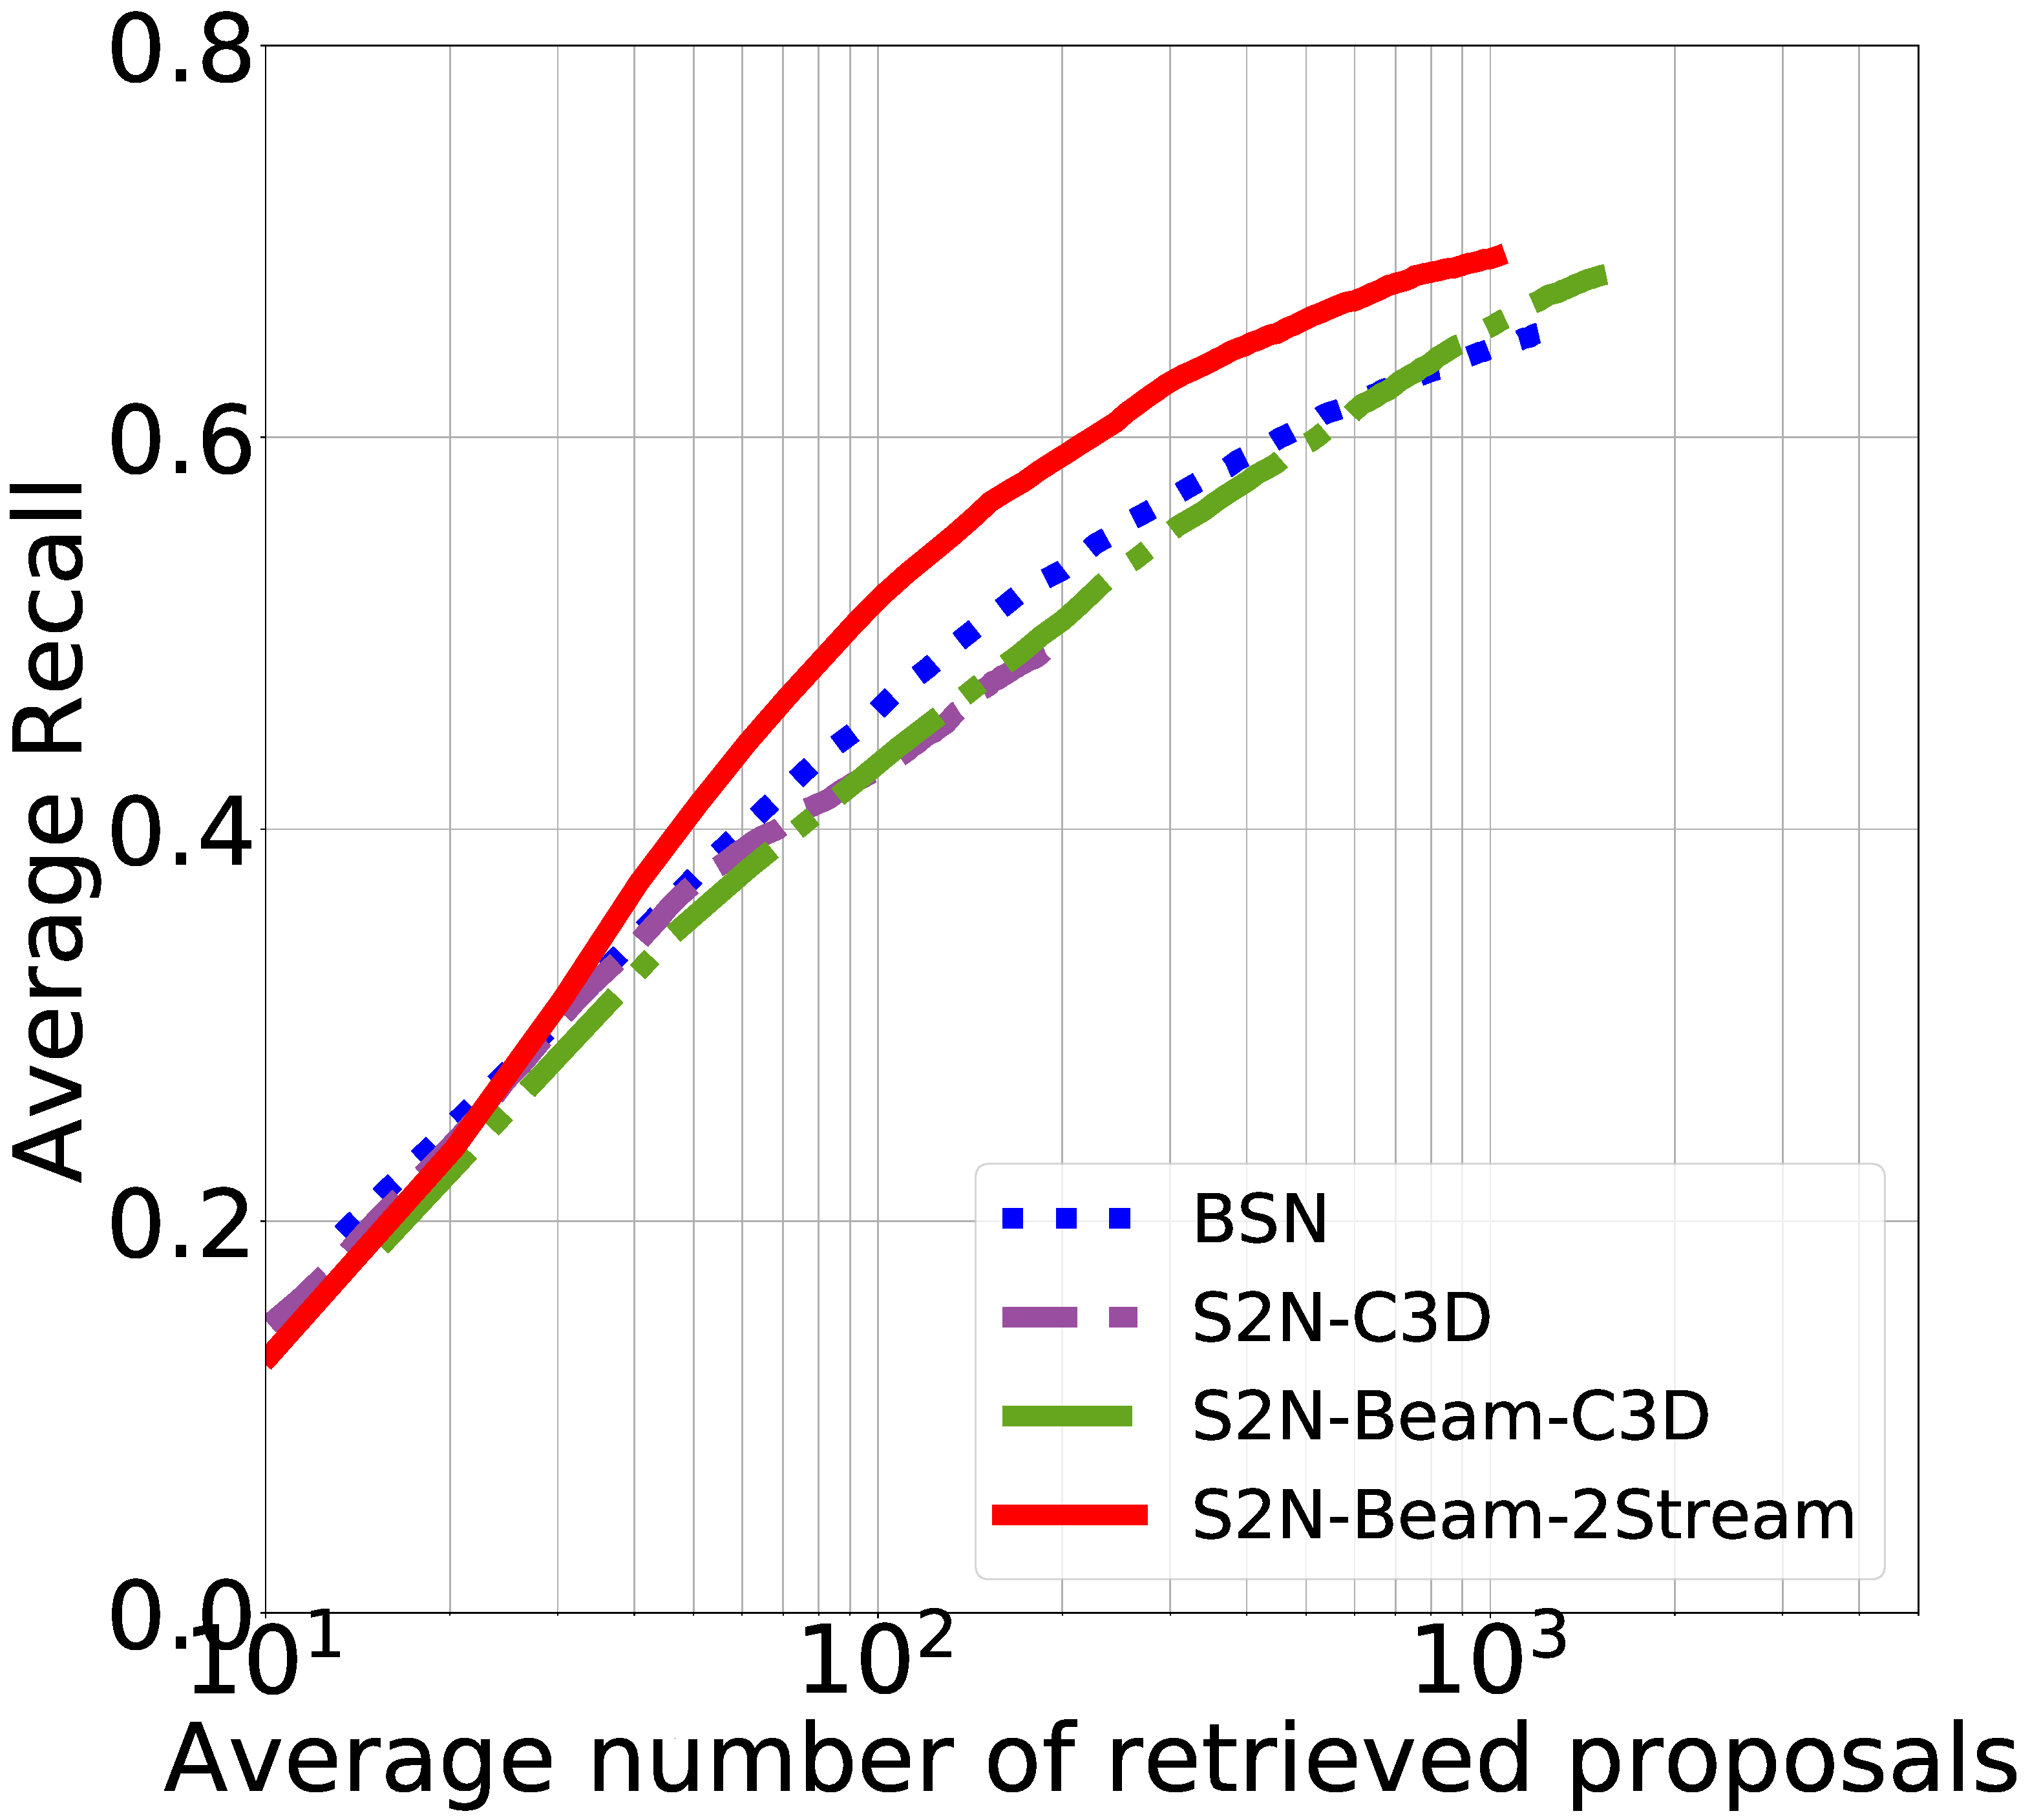
\includegraphics[width=\textwidth]{figures/results/S2N-Beam-2Stream_avg_recall.pdf}
    \caption{AR-N}
   	%\caption{easy cases}
   \end{subfigure}
   \begin{subfigure}[b]{0.24\textwidth}
   	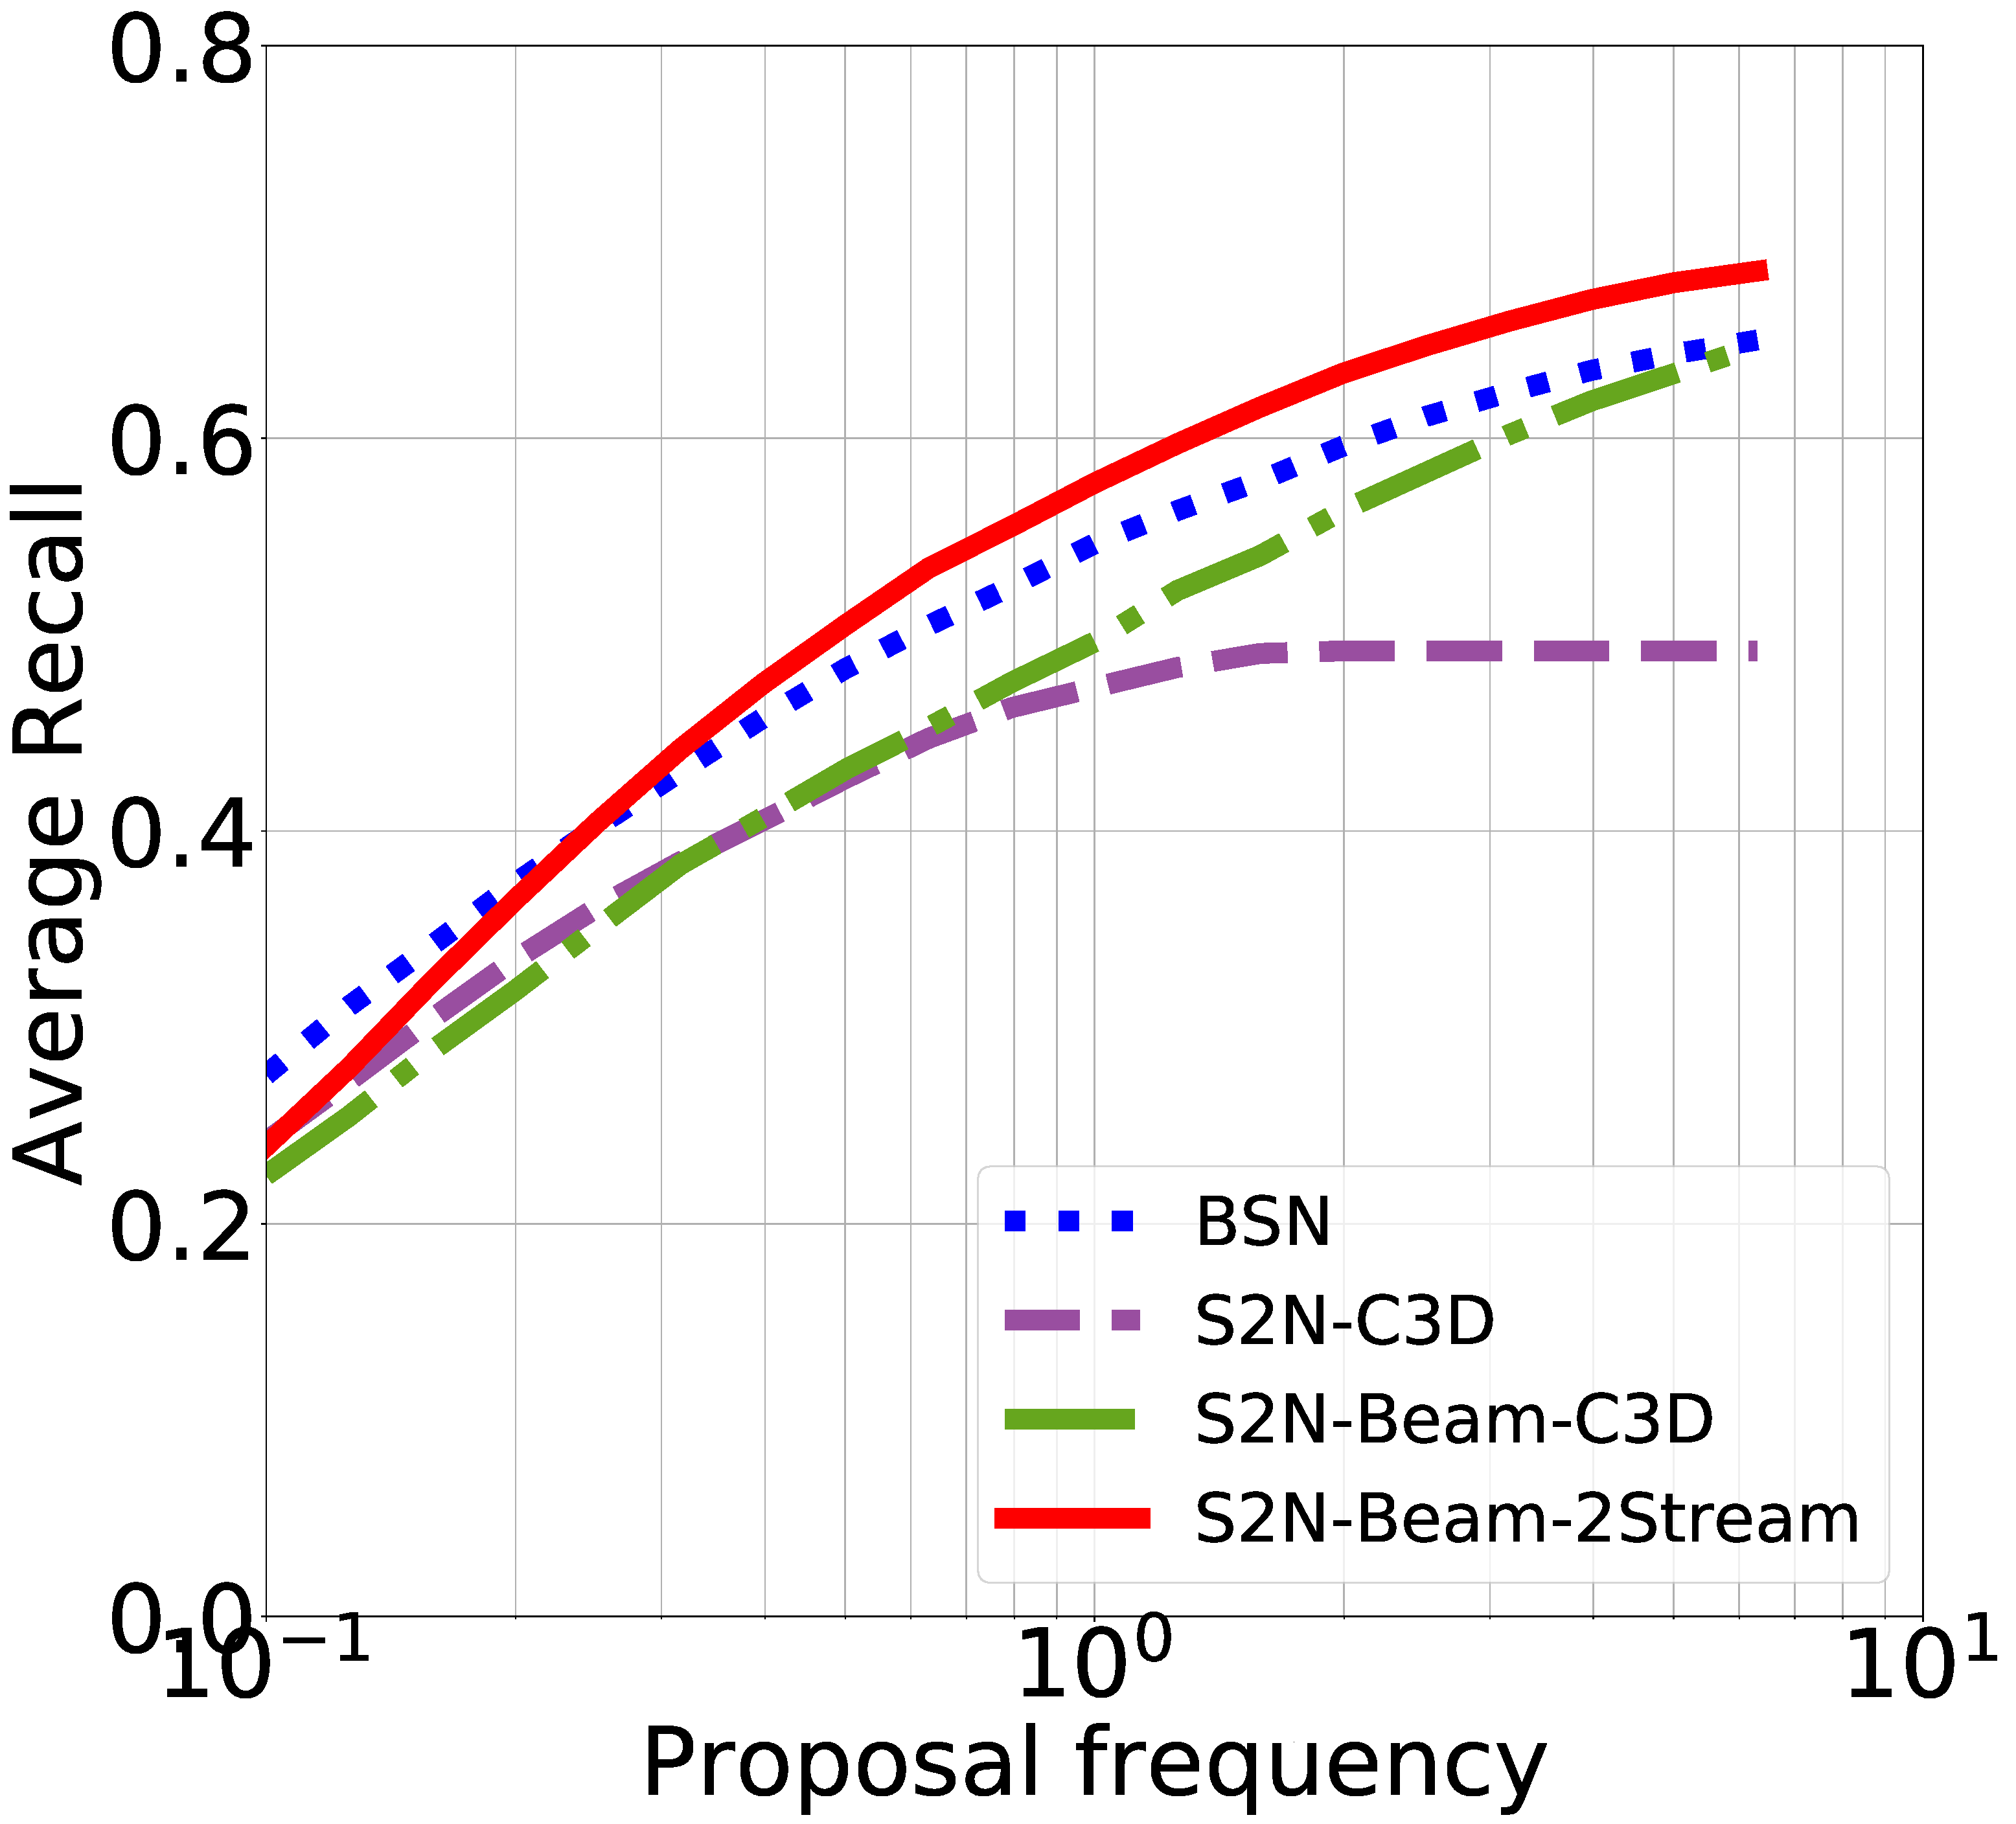
\includegraphics[width=\textwidth]{figures/results/S2N-Beam-2Stream_freq.pdf}
        \caption{AR-F}
   \end{subfigure}  
       \begin{subfigure}[b]{0.24\textwidth}
   	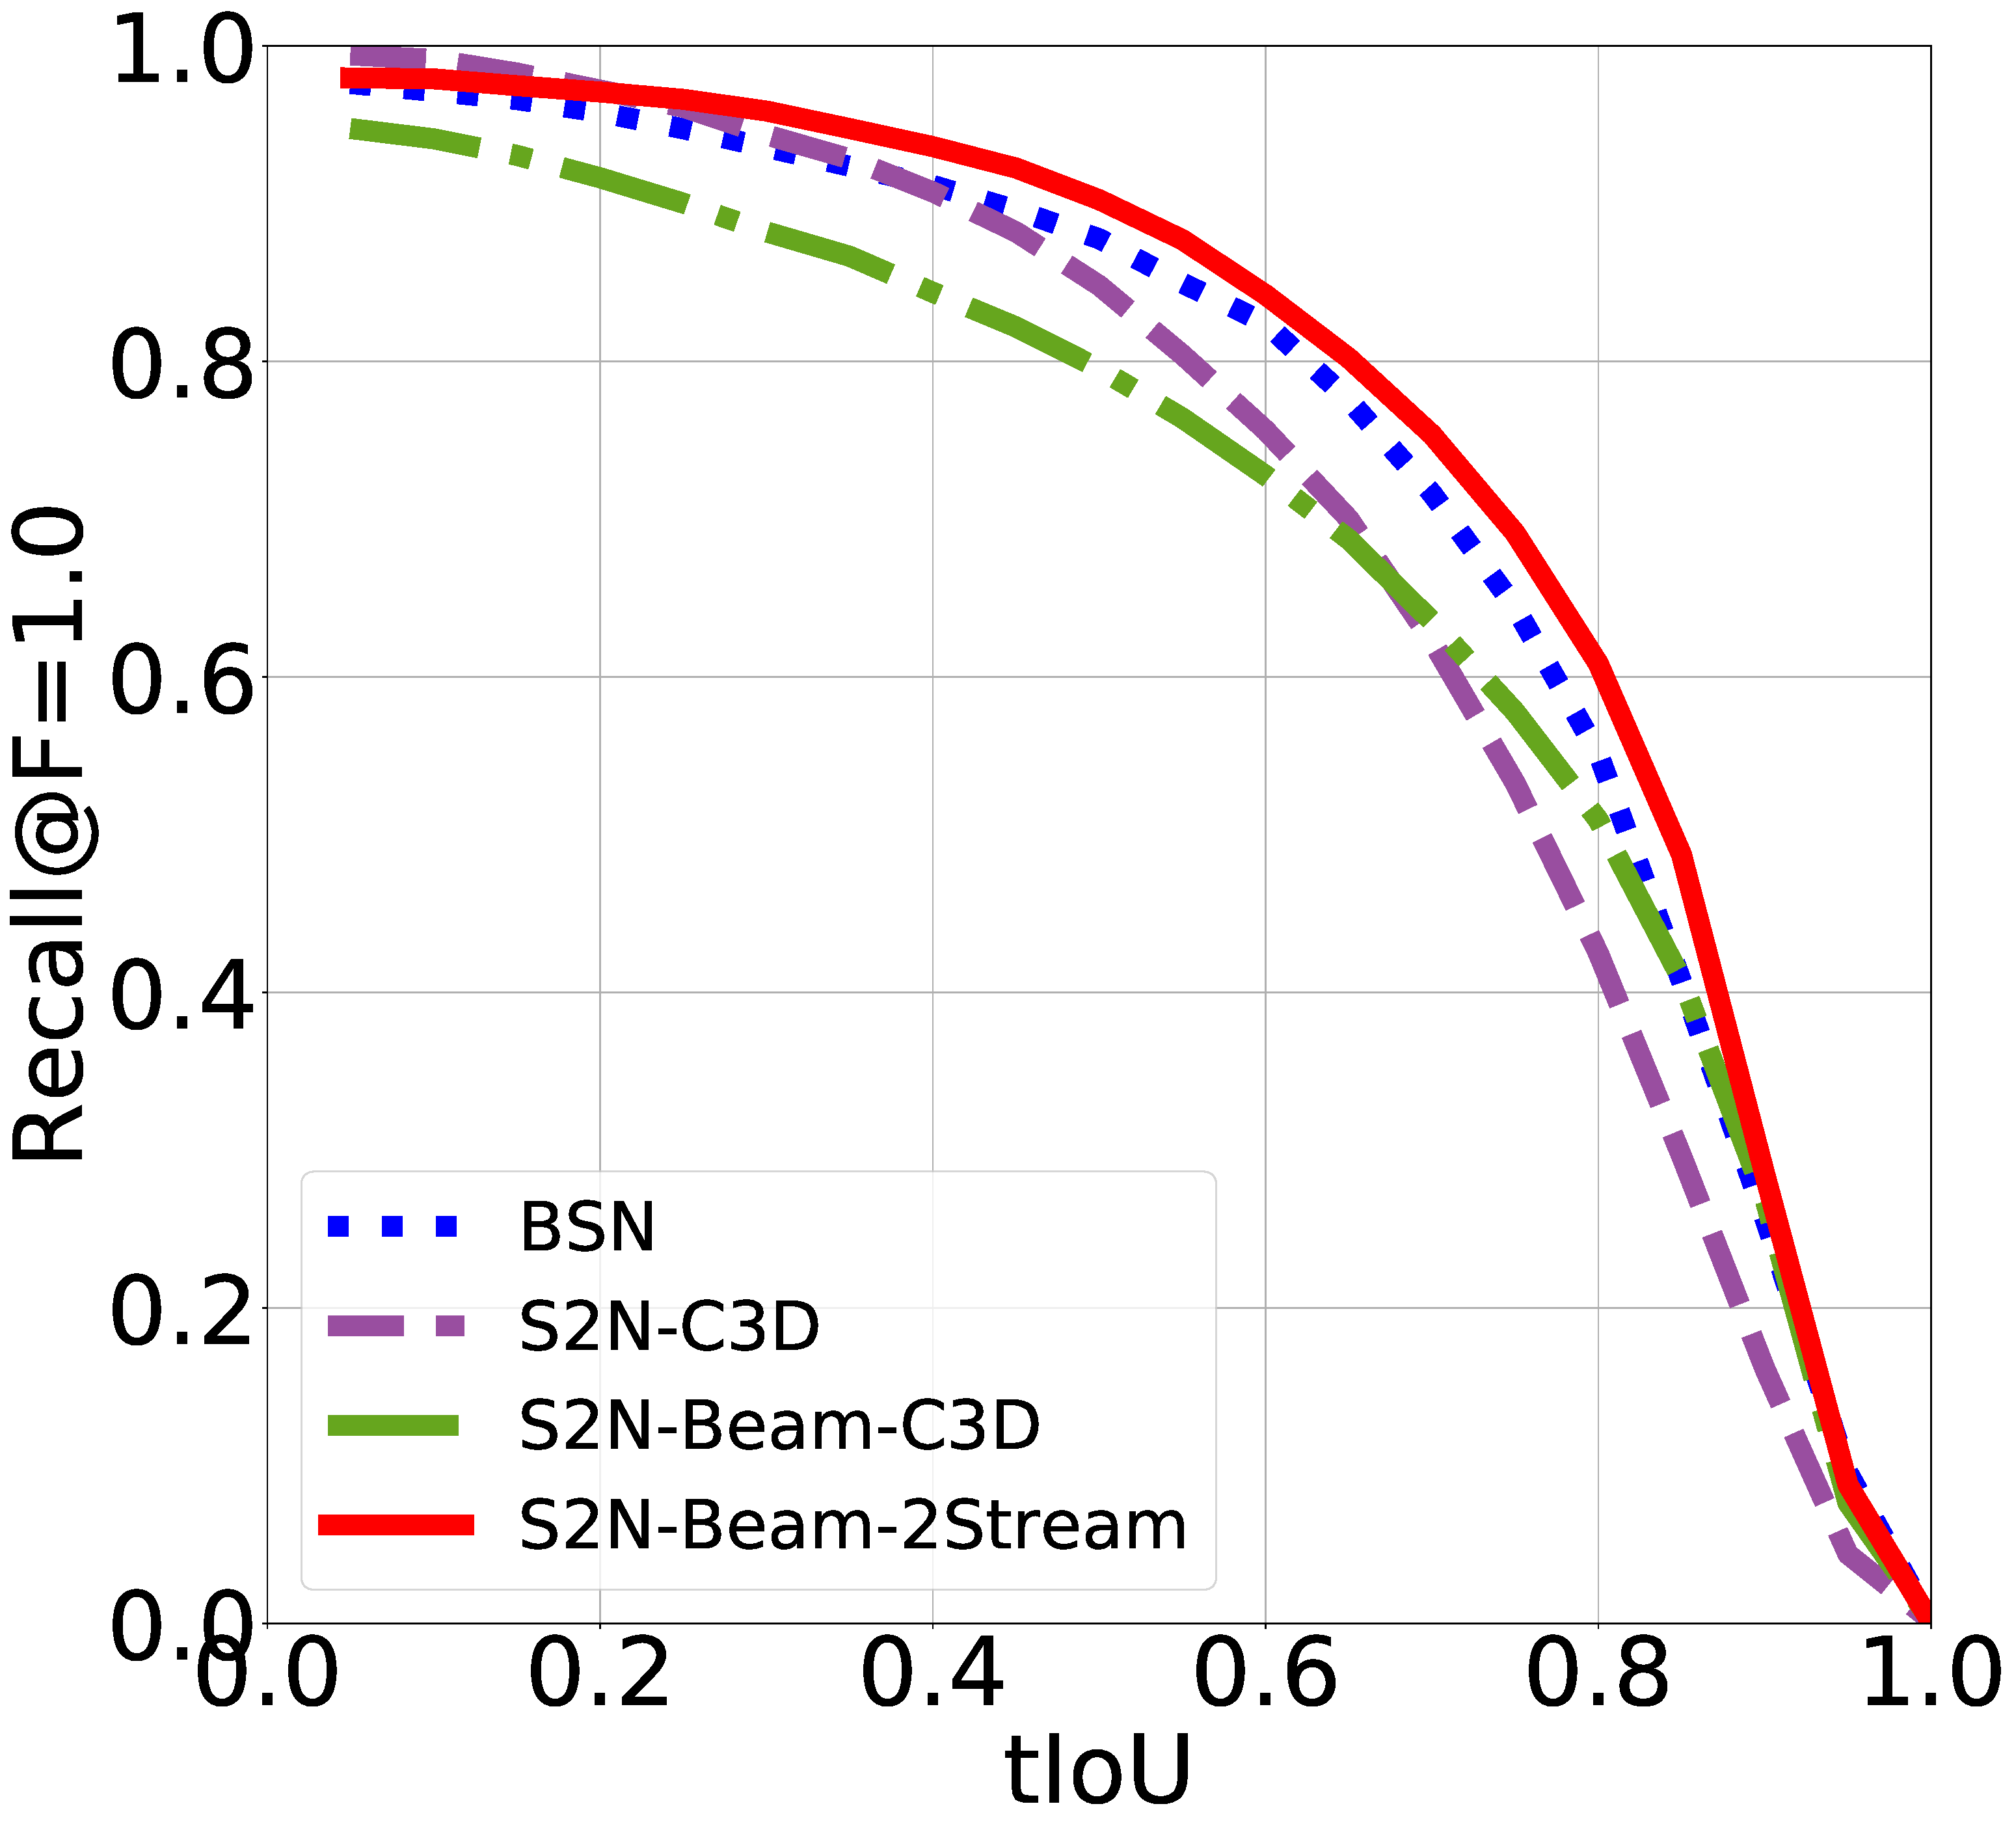
\includegraphics[width=\textwidth]{figures/results/S2N-Beam-2Stream_recall_freq.pdf}
    \caption{Recall@1.0-tIoU}
       \end{subfigure}  
        \begin{subfigure}[b]{0.24\textwidth}
    	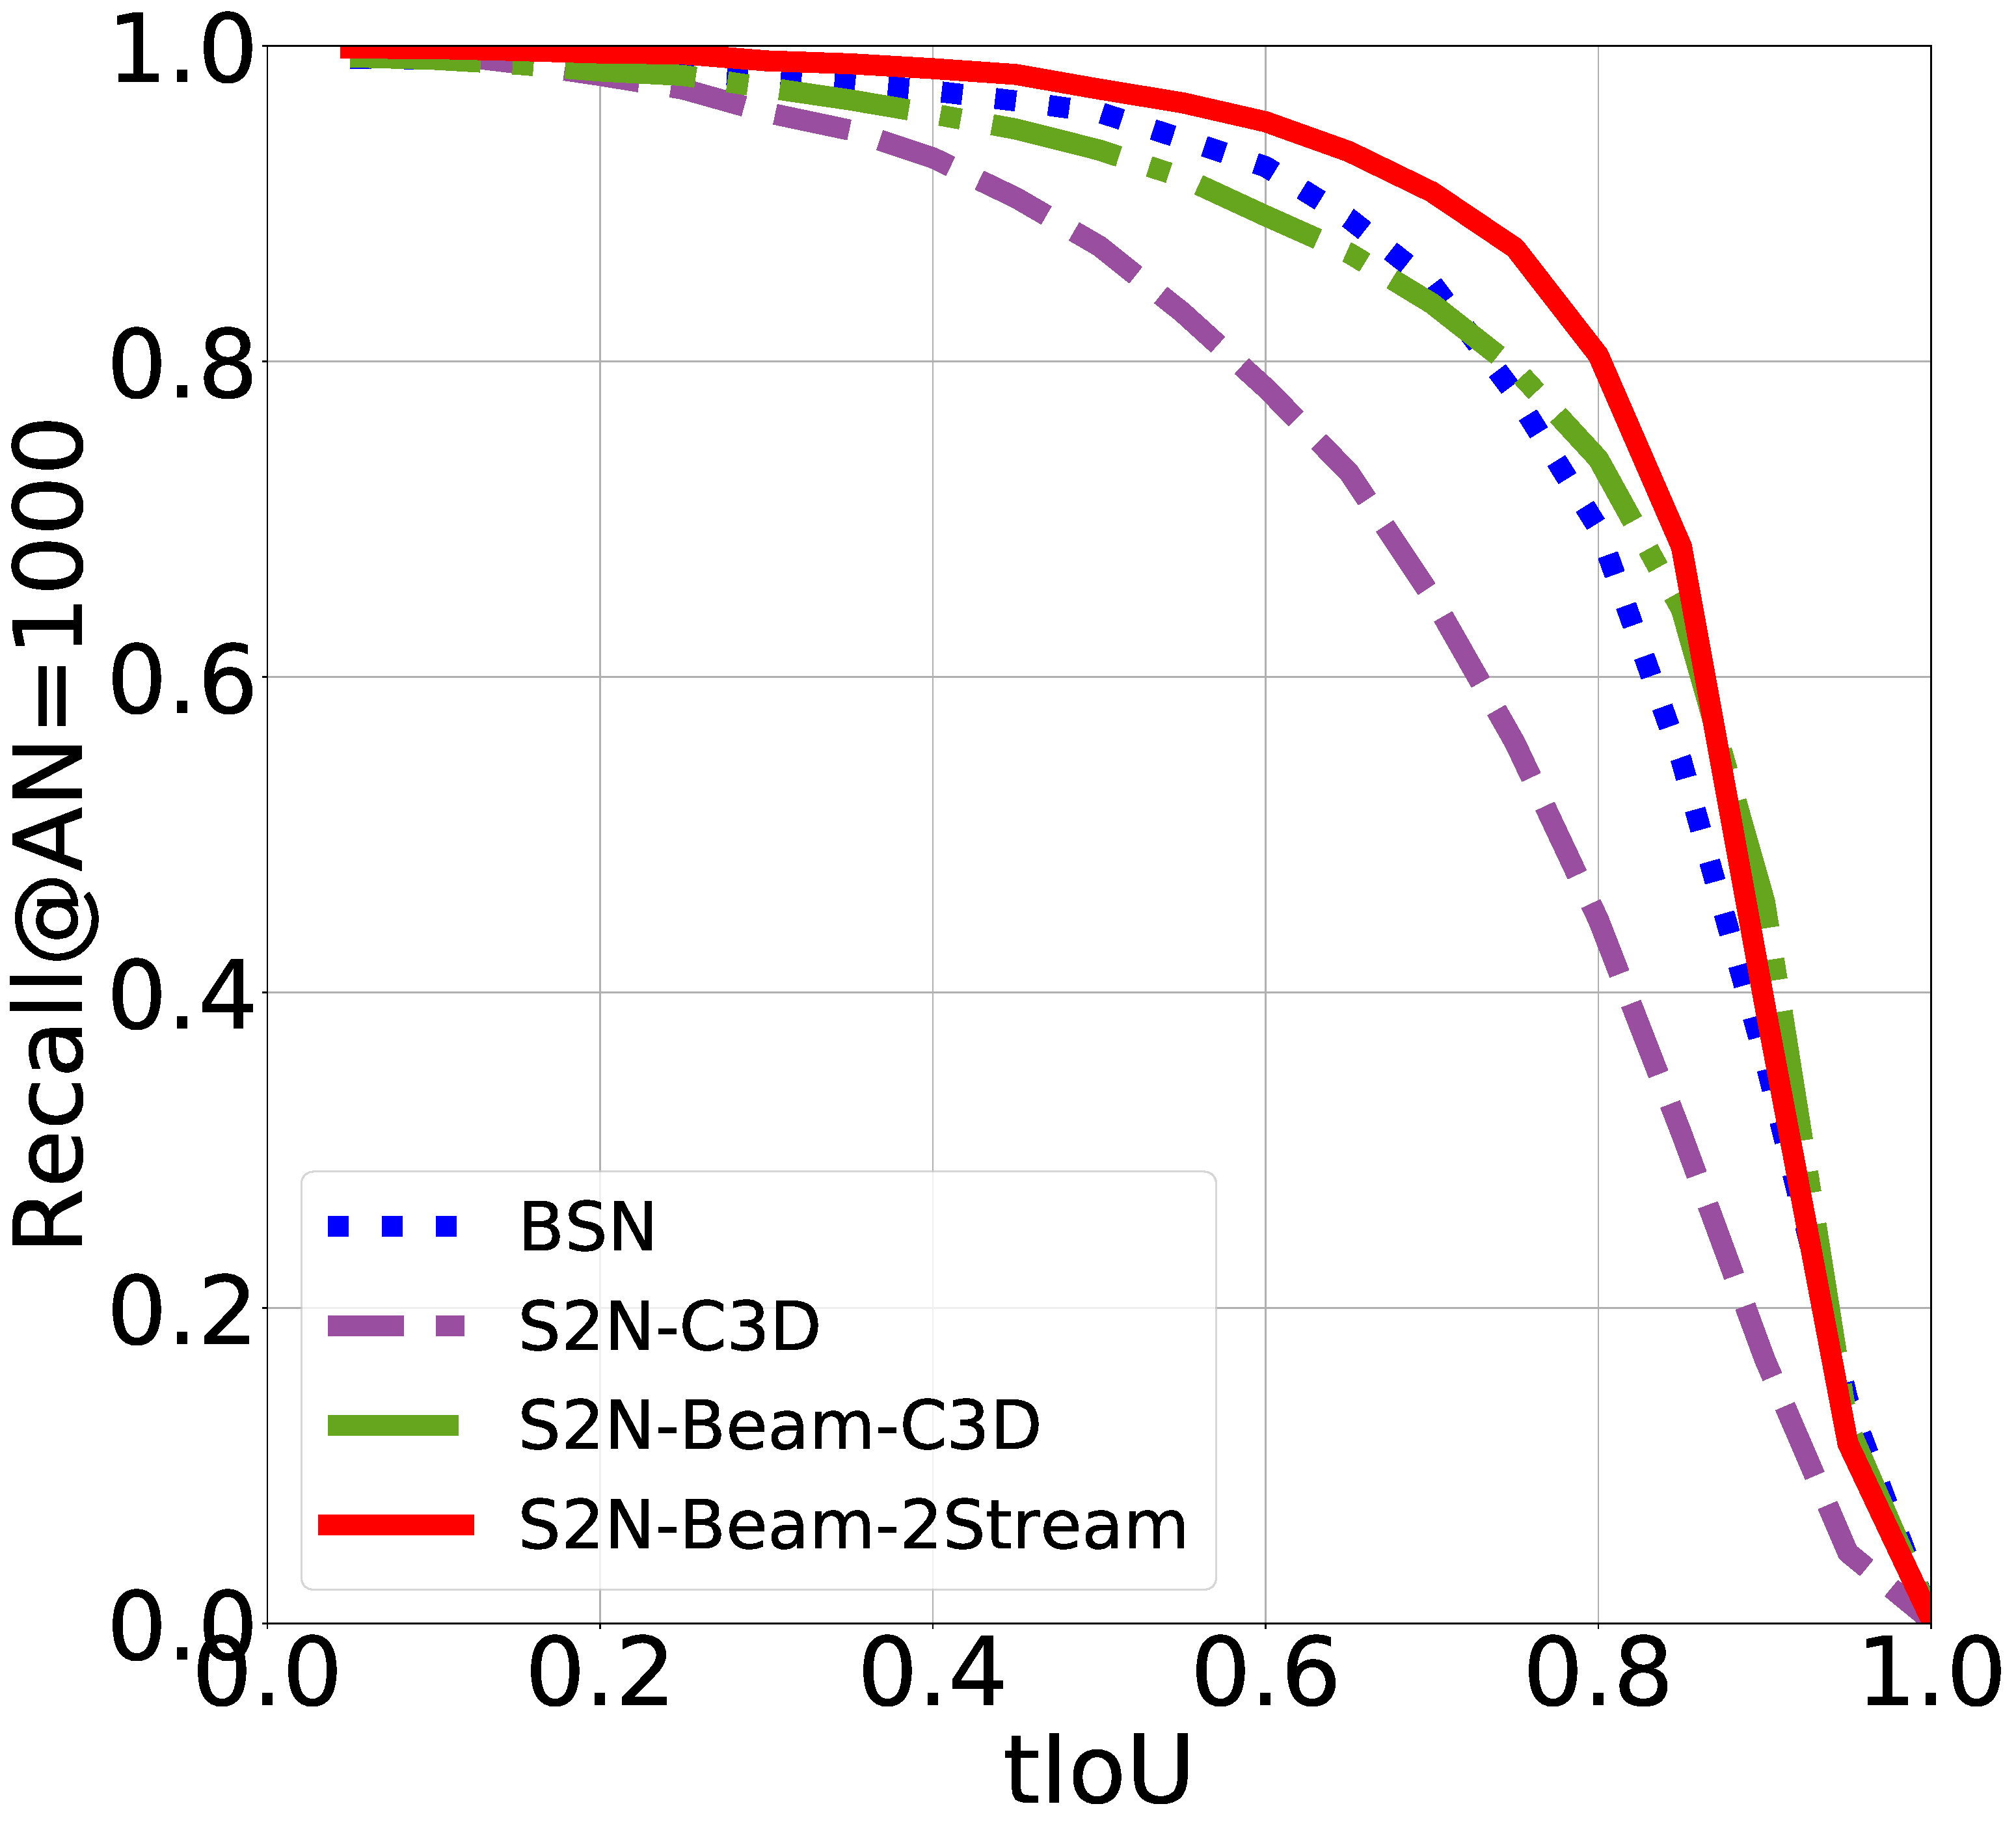
\includegraphics[width=\textwidth]{figures/results/S2N-Beam-2Stream_recall1000.pdf}
	\caption{Recal@N=1000\label{subfig:avg-recall-comp}}
    \end{subfigure}

   \caption{Comparison between variants of \S2N on THUMOS14. \S2N-Beam improve performance especially when proposal frequency is high. \S2N-Beam with two stream feature achieves best performance under various performance metrics. \label{fig:proposal-2stream}}   
\vspace{-.05in}
\end{figure*}



% The comparison to baselines under \textit{AR-N}, \textit{AR-F},  and \textit{Recall@F=1.0-tIoU} metrics are shown in Figure~\ref{fig:proposal-c3d}. \S2N outperforms the baselines by a significant margin over all the metrics. Note the gap between \S2N and DAPs partially implies the necessity of considering the contextual information and the superiority of the proposed pointing mechanism.  Also note that we did not apply any post processing such as using the action length distributions as priors~\cite{shou2016temporal,Gao_2017_ICCV}, merging neighboring proposals or boundary refinement~\cite{shou2017cdc,Gao_2017_ICCV} other than a simple non-maximum suppression step. 


% Additionally, we also computed the performance of \S2N using two-stream features as suggested by XXX, we show that with the same two stream features, \S2N does significantly better than XXX

% Recall that previously, for each decoding step, the segment was generated by finding the largest location of the X, 




% \myheading{Post-Processings.} We realized that for the video action proposal task, the goal is to achieve a higher average recall, which is slightly different than the previous, Additionally, it gives more toleration on redundant proposals. However, SDN is not designed primarily for this goal. 


% We combine the proposals from chunks, sort them by their scores, and apply a Non-Maximum Suppression (NMS) with a 75\% temporal intersection over union (tIoU). Note this is the \textbf{only} post-processing step used to address the overlap introduced in splitting the videos. We also have attempted to use variants of NMS such as the Soft-NMS, however, we find that Soft-NMS gives significantly worse results. We have also experimented with Soft-NMS but observed significant drop when the number of proposals increases to  (comparisons will be shown in supp). The reason is that compared to NMS, Soft-NMS do not encourage diversity in the proposals, thus lead to server overlap with XXX.




% \textit{FIX}: optimize the localization errors using cross-entropy classification loss as suggested in~\cite{vinyals2015pointer} and assign labels to predictions base on a fixed order matching).

% \textit{HUG}: optimize the localization errors with cross-entropy loss and assign labels to predictions base on the Hungarian matching algorithm described in Sec.~\ref{sec:alignment}.

% \textit{Greedy}: optimize the localization errors with the EMD loss as in Eq.~(\ref{eq:emd}) and assign labels based on the fixed order matching.

% \textit{TopK}: optimize the localization errors with the $L_2$ loss as an alternative to EMD loss and assign labels based on the fixed order matching or the Hungarian matching algorithm.

\subsection{Ablation Study on Assignment Strategies} 
We further explore the influence of different label assignment strategies on the performance of \S2Ns. Specifically we compare the proposed \S2N trained with HMLC matching strategy with the alternatives introduced in Section~\ref{sec:alternatives_intro}. As shown in Table~\ref{results:different_assign}, the \S2N model trained with HMLC consistently outperforms its variants over multiple ranges of output proposals.

\setlength{\tabcolsep}{10pt}
\begin{table}
\centering
\begin{tabular}{   l   c   c  c   c  c }
\toprule
  Method & @50 & @100 & @200 & @500 &  @1000\\
 \midrule
 Fix  & 31.44 & 41.75 & 49.23 & 57.82 & 61.92 \\ 
 Greedy  & 34.10 & 41.82 & 49.71 & 58.38 & 64.03 \\ 
 TopK & 35.90 & 42.98 & 51.52 & 58.62 & 62.55 \\ 
 HMLC & \textbf{36.80} & \textbf{44.23} & \textbf{52.11} & \textbf{59.59} & \textbf{64.46} \\ 
\bottomrule
\end{tabular}
\caption{Comparison of \S2N trained with different assignment strategies under metric AR-N. \S2N with with HMLC strategy outperforms the alternatives over different number of predefined proposals.\label{results:different_assign}}

% \setlength{\tabcolsep}{0.1cm}
%\vskip -0.1in
\end{table}



%\textbf{Post-Processing.}
%As the nature of action proposal is slightly different than video summarization. We make the following modifications to enlarge the number of proposals.





%The \S2N performance  is likely to be further improved by replacing the C3D feature with more powerful representations (\emph{e.g.}, I3D~\cite{carreira2017quo}). We leave this for  future work.

%  (Should we say something about the principles in the baselines? E.g. the performance gain over DAPs is that we consider the context information ...What else do we need?)
%\begingroup
%\setlength{\intextsep}{-3pt}%

%\endgroup 





%\added[id=ZJ]{







% \subsection{\added[id=ZJ]{Video Action Detection}}


%We could not evaluate \S2N on TVSum~\cite{song2015tvsum}, because the annotations of TVSum were collected based on predefined segments that ignore natural boundaries and the task was formulated as a classification problem on these segments, which is not suitable for evaluating our model.


\section{Conclusions and Future Work}
We have proposed the Sequence-to-Segments Network (\S2N), a novel architecture that uses Segment Detection Units (SDU) to detect segments sequentially from an input sequence. We have shown that \S2N can be applied to real-world problems and achieve state-of-the-art performance.

There are a a few directions for future work. One direction is to augment the encoding stage to be capable of recording longer sequences~\cite{li2018independently}. Another possible direction is to extend \S2N to more complex problems such as action detection in untrimmed videos. A third  direction is to introduce auxiliary losses to enforce explicit semantic constraints on \S2N~\cite{buch2017end}.  It is also possible to base \S2N on the fully convolutional encoder-decoder architecture~\cite{gehring2017convolutional,vaswani2017attention}. 

%\myheading{Acknowledgements.} This project was partially supported by NSF-CNS-1718014, NSF-IIS-1763981, NSF-IIS-1566248, the Partner University Fund, the SUNY2020 Infrastructure Transportation Security Center, and a gift from Adobe.
%



%\subsection{Subsection Heading Here}
%Subsection text here.
%
%% needed in second column of first page if using \IEEEpubid
%%\IEEEpubidadjcol
%
%\subsubsection{Subsubsection Heading Here}
%Subsubsection text here.


% An example of a floating figure using the graphicx package.
% Note that \label must occur AFTER (or within) \caption.
% For figures, \caption should occur after the \includegraphics.
% Note that IEEEtran v1.7 and later has special internal code that
% is designed to preserve the operation of \label within \caption
% even when the captionsoff option is in effect. However, because
% of issues like this, it may be the safest practice to put all your
% \label just after \caption rather than within \caption{}.
%
% Reminder: the "draftcls" or "draftclsnofoot", not "draft", class
% option should be used if it is desired that the figures are to be
% displayed while in draft mode.
%
%\begin{figure}[!t]
%\centering
%\includegraphics[width=2.5in]{myfigure}
% where an .eps filename suffix will be assumed under latex, 
% and a .pdf suffix will be assumed for pdflatex; or what has been declared
% via \DeclareGraphicsExtensions.
%\caption{Simulation results for the network.}
%\label{fig_sim}
%\end{figure}

% Note that the IEEE typically puts floats only at the top, even when this
% results in a large percentage of a column being occupied by floats.
% However, the Computer Society has been known to put floats at the bottom.


% An example of a double column floating figure using two subfigures.
% (The subFiguresty package must be loaded for this to work.)
% The subfigure \label commands are set within each subfloat command,
% and the \label for the overall figure must come after \caption.
% \hfil is used as a separator to get equal spacing.
% Watch out that the combined width of all the subfigures on a 
% line do not exceed the text width or a line break will occur.
%
%\begin{figure*}[!t]
%\centering
%\subfloat[Case I]{\includegraphics[width=2.5in]{box}%
%\label{fig_first_case}}
%\hfil
%\subfloat[Case II]{\includegraphics[width=2.5in]{box}%
%\label{fig_second_case}}
%\caption{Simulation results for the network.}
%\label{fig_sim}
%\end{figure*}
%
% Note that often IEEE papers with subfigures do not employ subfigure
% captions (using the optional argument to \subfloat[]), but instead will
% reference/describe all of them (a), (b), etc., within the main caption.
% Be aware that for subFiguresty to generate the (a), (b), etc., subfigure
% labels, the optional argument to \subfloat must be present. If a
% subcaption is not desired, just leave its contents blank,
% e.g., \subfloat[].


% An example of a floating table. Note that, for IEEE style tables, the
% \caption command should come BEFORE the table and, given that table
% captions serve much like titles, are usually capitalized except for words
% such as a, an, and, as, at, but, by, for, in, nor, of, on, or, the, to
% and up, which are usually not capitalized unless they are the first or
% last word of the caption. Table text will default to \footnotesize as
% the IEEE normally uses this smaller font for tables.
% The \label must come after \caption as always.
%
%\begin{table}[!t]
%% increase table row spacing, adjust to taste
%\renewcommand{\arraystretch}{1.3}
% if using array.sty, it might be a good idea to tweak the value of
% \extrarowheight as needed to properly center the text within the cells
%\caption{An Example of a Table}
%\label{table_example}
%\centering
%% Some packages, such as MDW tools, offer better commands for making tables
%% than the plain LaTeX2e tabular which is used here.
%\begin{tabular}{|c||c|}
%\hline
%One & Two\\
%\hline
%Three & Four\\
%\hline
%\end{tabular}
%\end{table}


% Note that the IEEE does not put floats in the very first column
% - or typically anywhere on the first page for that matter. Also,
% in-text middle ("here") positioning is typically not used, but it
% is allowed and encouraged for Computer Society conferences (but
% not Computer Society journals). Most IEEE journals/conferences use
% top floats exclusively. 
% Note that, LaTeX2e, unlike IEEE journals/conferences, places
% footnotes above bottom floats. This can be corrected via the
% \fnbelowfloat command of the stfloats package.




%\section{Conclusion}
%The conclusion goes here.





% if have a single appendix:
%\appendix[Proof of the Zonklar Equations]
% or
%\appendix  % for no appendix heading
% do not use \section anymore after \appendix, only \section*
% is possibly needed

% use appendices with more than one appendix
% then use \section to start each appendix
% you must declare a \section before using any
% \subsection or using \label (\appendices by itself
% starts a section numbered zero.)
%


%\appendices
%\section{Proof of the First Zonklar Equation}
%Appendix one text goes here.

% you can choose not to have a title for an appendix
% if you want by leaving the argument blank
%\section{}
%Appendix two text goes here.


% use section* for acknowledgment
\ifCLASSOPTIONcompsoc
  % The Computer Society usually uses the plural form
  \section*{Acknowledgments}
\else
  % regular IEEE prefers the singular form
  \section*{Acknowledgment}
\fi


This project was partially supported by NSF-CNS-1718014, NSF-IIS-1763981, NSF-IIS-1566248, the Partner University Fund, the SUNY2020 Infrastructure Transportation Security Center, and a gift from Adobe.





% Can use something like this to put references on a page
% by themselves when using endfloat and the captionsoff option.
\ifCLASSOPTIONcaptionsoff
  \newpage
\fi



% trigger a \newpage just before the given reference
% number - used to balance the columns on the last page
% adjust value as needed - may need to be readjusted if
% the document is modified later
%\IEEEtriggeratref{8}
% The "triggered" command can be changed if desired:
%\IEEEtriggercmd{\enlargethispage{-5in}}

% references section

% can use a bibliography generated by BibTeX as a .bbl file
% BibTeX documentation can be easily obtained at:
% http://mirror.ctan.org/biblio/bibtex/contrib/doc/
% The IEEEtran BibTeX style support page is at:
% http://www.michaelshell.org/tex/ieeetran/bibtex/
%\begin{thebibliography}{1}
%
\bibliographystyle{IEEEtran}
% argument is your BibTeX string definitions and bibliography database(s)
\bibliography{longstrings,egbib,pubs}
%\end{thebibliography}

%
% <OR> manually copy in the resultant .bbl file
% set second argument of \begin to the number of references
% (used to reserve space for the reference number labels box)
%\begin{thebibliography}{1}
%
%\bibitem{IEEEhowto:kopka}
%H.~Kopka and P.~W. Daly, \emph{A Guide to \LaTeX}, 3rd~ed.\hskip 1em plus
%  0.5em minus 0.4em\relax Harlow, England: Addison-Wesley, 1999.
%
%%\end{thebibliography}
%\small
%\bibliographystyle{ieee}
%%\bibliographystyle{abbrvnat}
%\bibliography{longstrings,egbib,pubs}
% biography section
% 
% If you have an EPS/PDF photo (graphicx package needed) extra braces are
% needed around the contents of the optional argument to biography to prevent
% the LaTeX parser from getting confused when it sees the complicated
% \includegraphics command within an optional argument. (You could create
% your own custom macro containing the \includegraphics command to make things
% simpler here.)
%\begin{IEEEbiography}[{\includegraphics[width=1in,height=1.25in,clip,keepaspectratio]{mshell}}]{Michael Shell}
% or if you just want to reserve a space for a photo:

 \begin{IEEEbiography}[{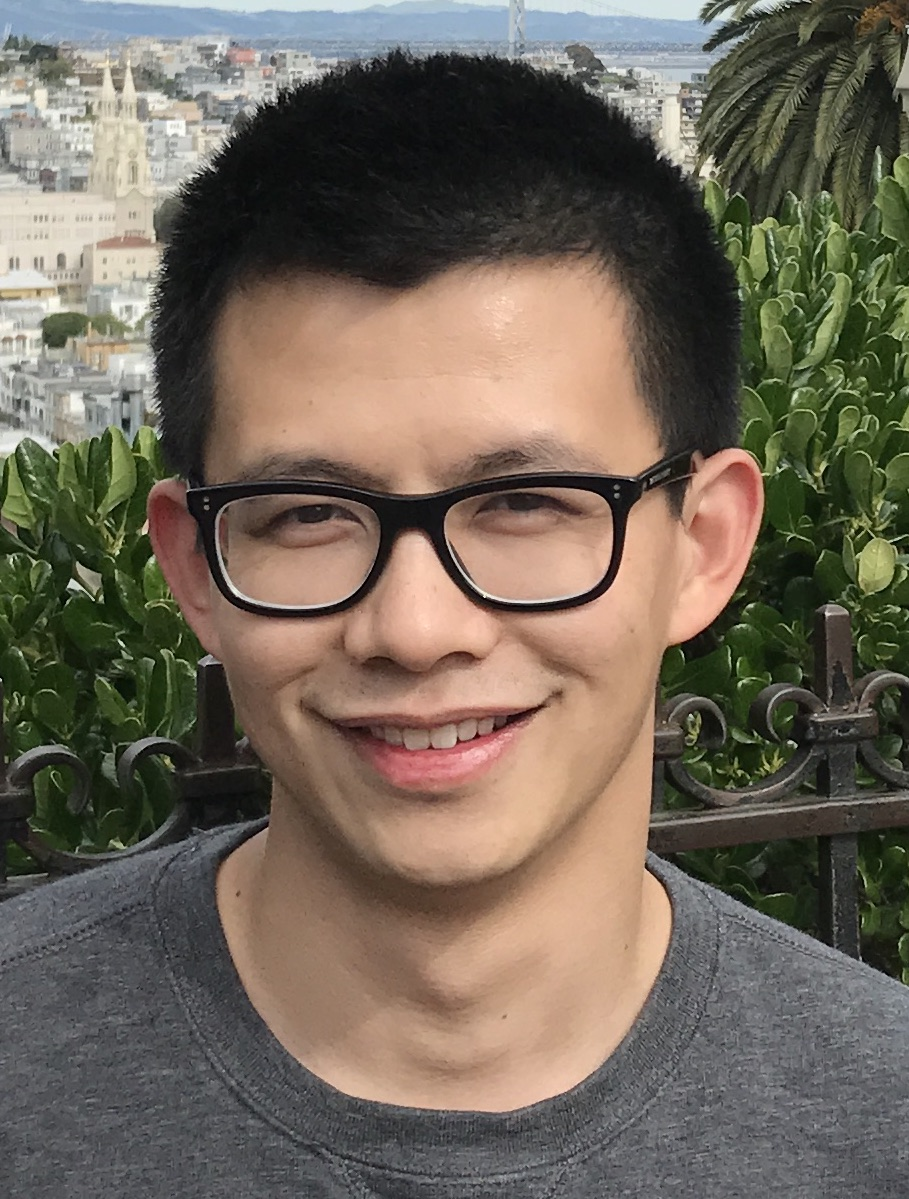
\includegraphics[width=1in,height=1.2in,clip,keepaspectratio]{figures/biograph/ZijunWei-Head-2017-sm.jpg}}]{Zijun Wei} received a Bachelor of Network Engineering from Nanjing University of Science and Technology in 2011 and a Master of Robotics from Carnegie Mellon University in 2013. He is currently a PhD candidate at the Department of Computer Science, Stony Brook University. His research focuses on visual saliency and human preference modeling. 
\end{IEEEbiography}

 \begin{IEEEbiography}[{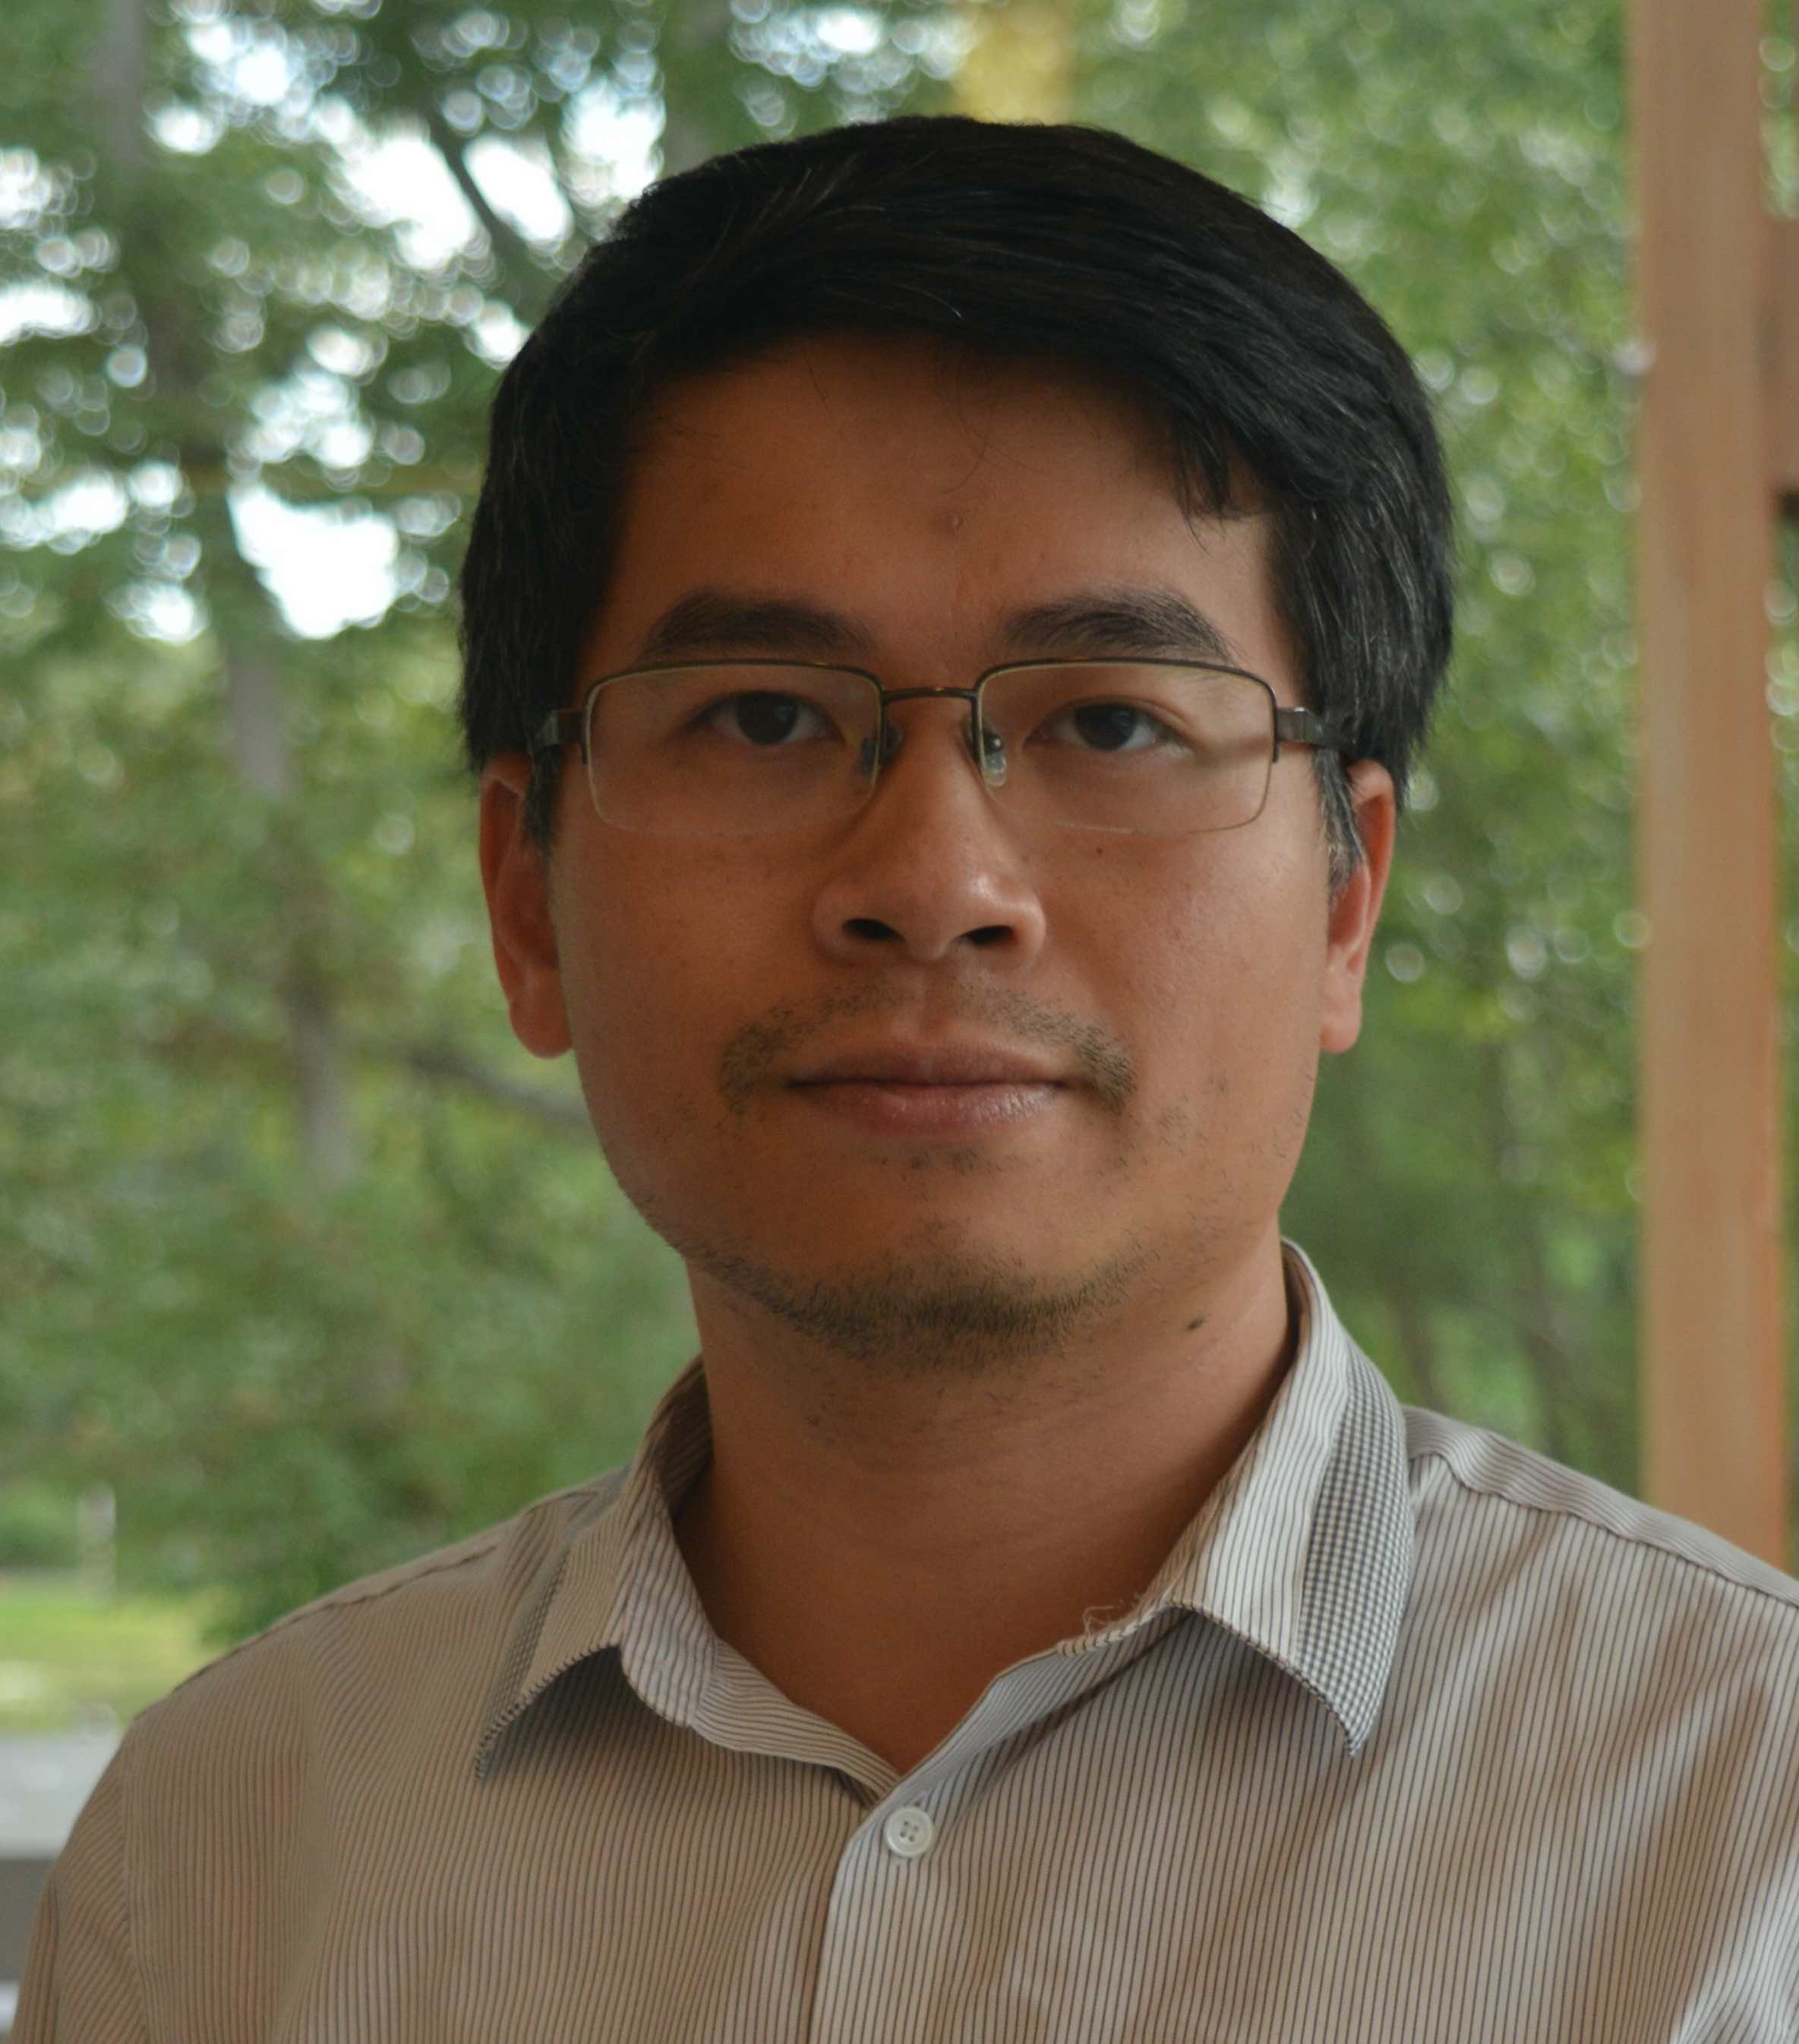
\includegraphics[width=1in,height=1.2in,clip,keepaspectratio]{figures/biograph/MinhHoaiNguyen_headshot_2017_sm.jpg}}]{Minh Hoai}
is an Assistant Professor of Computer Science at Stony Brook University. He received a Bachelor of Software Engineering from the University of New South Wales in 2005 and a Ph.D. in Robotics from Carnegie Mellon University in 2012. His research interests are in computer vision and machine learning, especially human action and activity recognition and prediction. 
\end{IEEEbiography}

% if you will not have a photo at all:
\begin{IEEEbiographynophoto}{John Doe}
Biography text here.
\end{IEEEbiographynophoto}

% insert where needed to balance the two columns on the last page with
% biographies
%\newpage


\begin{IEEEbiographynophoto}{Jane Doe}
Biography text here.
\end{IEEEbiographynophoto}

% You can push biographies down or up by placing
% a \vfill before or after them. The appropriate
% use of \vfill depends on what kind of text is
% on the last page and whether or not the columns
% are being equalized.

%\vfill

% Can be used to pull up biographies so that the bottom of the last one
% is flush with the other column.
%\enlargethispage{-5in}



% that's all folks
\end{document}


